\documentclass[12pt,a4paper,titlepage]{report}

\usepackage{times}

\usepackage[utf8]{inputenc}
\usepackage[T1]{fontenc}
\usepackage[english]{babel}

\usepackage{setspace}
\onehalfspacing

\usepackage[hidelinks]{hyperref}

\usepackage{graphicx}

\usepackage{minted}
%TODO: remove red box on parser error

\setminted{baselinestretch=1,fontsize=\footnotesize}

\usepackage{caption}

\usepackage{algorithm} %[plain] ?
\usepackage{algpseudocode}
\makeatletter
\renewcommand*{\ALG@name}{Pseudocode}
\makeatother

\usepackage{multirow}

% avoid floats moving outside the sections
\usepackage[section]{placeins}

% margini de 1 inch peste tot
\usepackage[margin=1in]{geometry}

\usepackage{amsmath}

%\usepackage{draftwatermark}
%\SetWatermarkText{Draft}
%\SetWatermarkScale{1}

\author{Barbu Paul - Gheorghe}

%TODO: coperta

\begin{document}

\begin{titlepage}
{
	\centering
	\textbf{"Lucian Blaga" University of Sibiu – Romania} \\
}

{
	\centering
		\textbf{Faculty of Engineering} \\
}

{
	\centering
		\textbf{Master program:} Advanced Computing Systems \\
}


\vfill

{
	\centering
	\Large
	\textbf{DISSERTATION} \\
}

{
	\centering
	\Large
	Forecasting electricity consumption and production using ARIMA time series models \\
}

\vfill

{
	\centering
		\textbf{Graduate:} Barbu Paul - Gheorghe\\
		\textbf{Scientific coordinator:} Conf. dr. ing. Árpád GELLÉRT \\
}

\vfill

{
	\centering
	2019 \\
}
\end{titlepage}

\tableofcontents
\newpage

\subsection*{Abstract}

The current dissertation thesis aims to develop an understanding of time series forecasting principles, with an emphasis on the Auto Regressive Integrated Moving Average algorithm (or ARIMA for short), in the energy consumption field. The aim is also to develop a software implementation that uses the ARIMA model in order to easily forecast a given time series and to be able to analyze the results and decide if the chosen model is properly predicting the data or not.

Electric energy consumption is something that we take for granted. Even if actively consuming electricity while using a desktop computer, by lightning our rooms or by passively consuming electric energy while our smart-phones are in standby mode it is safe to say that we use electric energy all the time. That is, without even considering industrial use-cases, where up times of 24 hours 7 days a week are expected from most factories. As such, I consider that electricity is a much needed depletable resource and, as is the case with any such resource that we have to generate, we also have to know how we use it in order to better manage it.

Considering the fact that electricity domestic consumption has been steadily increasing (with the exception of 2009, maybe because of the financial crisis and other hard to explain factors) \cite{enerdata} for the world as a whole, it is past time to take note of our consumption patterns and start adapting them in order to reduce the footprint we leave on the medium and to minimize the waste of electrical energy, which cannot be reliably stored in high amounts.

Hence this work focuses on finding the patterns in the electrical energy consumption and predicting them using ARIMA models, with the hopes that being able to tell how consumers will use the energy in the near future, home owners, companies and governments may optimize their behavior and the import and export of electricity.

This work will focus on a single set of data for making the forecasts about energy consumption, although the principles, models and the way of thinking presented herein should be general enough to be applicable for other time-series data sets that are out there. What will change is, of course, the parameters given to the used ARIMA models and the interpretation of the results.

The Auto Regressive Integrated Moving Average algorithm was chosen to make the predictions since it is a combination of several other models and can generalize them, covering a wide range of possibilities through its parameters. Being a very general algorithm for time-series predictions it is also widely used, not only for electric energy consumption \cite{bouzerdoum}, but also for finance and socio-political data \cite{fpp2}.

This work will present how the ARIMA models work and the statistical machinery around them from my experience while forecasting one data set, comprised of five different time-series. The data set has been used in other works as well, one of which was done here at "Lucian Blaga" University of Sibiu, in the same department. The paper, called "Loads management based on Photovoltaic and Energy Storage System" \cite{feilmeier}, studies the very same idea that I set out to study in this work, the difference being that the author uses artificial neural networks to model and predict the given data. So given the fact that this data has already been analyzed, we have the opportunity for comparing the performance of Artificial Neural Networks, computed by Stefan Feilmeier, with the performance of ARIMA, computed in this paper by myself.

The five time-series in the dataset are all gathered at the same time, starting with the beginning of year 2015 on 1st of January. Each data point represents the current Watt usage of a home, gathered every five minutes during a period of five months, so until the month of May 2015 (inclusive), tallying up to around 150 days of data, each consisting of 288 individual sampling points. Although there is plenty of data to work with, only three of the time-series represent actual consumption, on each of the three phases of three phase current (Ph1, Ph2 and Ph3). The other two time-series (namely: PV1 and PV2) are actually the number of Watts produced by two photo-voltaic panels mounted on the same house.
Because of the nature of the data, there should be no difference in forecasting the two groups of time-series, it doesn't matter if the energy is gathered or consumed, the prediction work-flow and mechanisms used in this paper should remain generally applicable, only the semantics of the conclusions will change, instead of saying "I predict there will be consumed X Watts over the next period of time", one would instead say: "I predict there will be generated X Watts of energy over the next period of time".

The current state of the time-series algorithms and available statistical tools in the programming communities have pushed me to use the R programming language \footnote{\url{https://www.r-project.org/}} in order to carry out the task of this dissertation paper, because R seems to be the best and among the most used \cite{Rdesign} choice for interactive analysis of data and statistical studies, having over 13000 (thirteen thousand) packages available online\footnote{At the beginning of 2019, according to: \url{https://cran.r-project.org/web/packages/}}, packages that can be used to carry out different tasks, from string manipulation and XML parsing, to forecasting time-series data.

So this paper aims at creating a functional software implementation using the R programming language and its rich ecosystem in statistical tools (of which I use ARIMA models) for forecasting the electrical energy consumption for a household over a predetermined period of time. By the end of the paper the reader will conclude that the goal has been successfully achieved and a variation on the ARIMA algorithm is indeed suited for forecasting electrical energy demand time-series such as the ones used here. The results are favorable compared to those produced by the ANN method, but not by much compared to some benchmark algorithms which are much simpler in terms of mathematical complexity and shorter in term of both implementation and running time.

\newpage
\chapter{Theoretical considerations}
\section{Introduction and etymology}

The verb "to forecast" means "to predict" or "to estimate" a future event or trend \cite{oxfordForecast}, when used as a noun it refers to the results of the verb, the data that has been estimated or predicted.

This paper has set as its goal to predict the electrical energy consumption and production of a modern house using the Auto Regressive Integrated Moving Average model, while at the same time understanding and presenting the algorithm and its constituent parts.

The underlaying problem that pushed me to choose this kind of a project is the fact that electrical energy cannot be stored in high amounts and, as a consequence, countries and governments need to understand the patterns of consumption and production of their residents in order to optimize the import and export of electrical energy. Through such optimizations the price of electricity could be reduced, which is a benefit to the domestic consumer.

We also have to keep in mind that there is an increase in electrical energy consumption worldwide, according to Enerdata \cite{enerdata} and their plot of electricity demand which can be seen in figure \ref{energytrend}. All the while there is an increasing interest for green energy, while forecasting in itself doesn't help on this front of the problem, it can help to predict which households might be suited for photo voltaic panels installation in order to further reduce the carbon dioxide footprint. 

\begin{figure}[h]
    \centering
    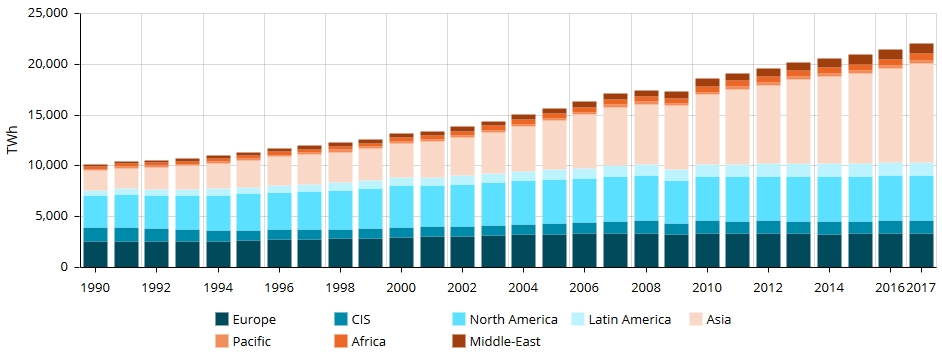
\includegraphics[width=1\textwidth]{denergytrend}
    \caption{Electrical Energy Consumption Trend}
    \label{energytrend}
\end{figure}

In what follows, apart from the word "forecasting" I will also use the words "model" and "algorithm". Most of the time I will use the two words interchangeably, for example "ARIMA model" or "ARIMA algorithm", but, if being pedantic is desired, their meaning is different since "model" refers to the mathematical or statistical model that is the basis for the later-developed algorithm. We can look at it this way: the model is the building block of the algorithm. The algorithm on the other hand being the series of steps taken to solve a particular problem.

In the end I'd like to be able to state that for a given time frame in the future a household will consume or generate a certain amount of energy with 80\% or even 95\% confidence.

\section{Structure of the dissertation}

The paper is arranged in two chapters, the present one, which aims to explain the theoretical concepts behind time-series forecasting using ARIMA and to give insights to the statistical concepts underlaying the decisions taken throughout the research phase.
This chapter should present the current state of the domain and the advances in forecasting time-series data, each concept occupying its own section. A cursory look at the R programming language and its ecosystem of statistical tools and Integrated Development Environments (or in short: IDEs) will be provided. Then an in depth explanation will be provided to each and every one of the main concepts involved in the process of forecasting electrical energy demand using the ARIMA model.

The second chapter shall disseminate the actual research work flow that I applied in solving the problem of electricity demand forecasting with ARIMA. The concepts explained in this second chapter are using the theoretical basis introduced in the first chapter.
Here I will present the results of my work and compare the ARIMA algorithm to previous work done on the same data but by using Artificial Neural Networks (or in short ANNs) by Stefan Feilmeier.

The second chapter will also shine some light on why R is one of the best tools to use in such a context, where easily accessible statistical instruments are of utmost importance. This will be accomplished by showing and explaining the key code snippets of the research, while to full source code will be available on the accompanying CD.

\section{State of the art in forecasting}

Considering the fact that energy production and consumption is so widespread it is very hard to quantify the exact state of the forecasting methods and tools used by the big electricity providers, mainly because of their variety, but also because of the trade secret nature with which such methods are treated. Basically being able to predict the future in any given domain, not only electricity production and consumption, also means that you can use that information to your advantage, hence the secret nature of the business. Still, saying that the methods presented herein are able to predict the future is not very accurate, what we can do is: we can analyze the past and from that data make inferences about the future, hypothesize about it with some degree of confidence.

Taking a bird's eye view of the problem, it is no different than what we are used to in weather forecasts. We can say for example with 60\% confidence that in the next several hours it will rain. This statement is bases on previous data that is at the meteorologists' disposal, data such as past rainfall quantities for the current season or even day and hour, the direction of the wind, the amount of clouds and the difference in air pressure in the area that they will forecast rain for.

Similarly, for electrical energy demand prediction we can have models that take into account several predictor variables, such as the time of day, the temperature, the season and maybe other social elements.
\begin{itemize}
    \item Time of day is important in prediction because in the case of electrical energy consumption we could imagine a scenario where the consumption would be highest in the morning when everyone gets ready for work or school and then decrease a bit, only to increase back again during the evenings when everybody returns home. The same logic applies to electricity production by photo-voltaic panels, their peak would be at noon, when the sun shies brightest and the light's angle of incidence is the widest;
    \item The outside temperature is also important in countries that mostly use electrical based heating and cooling. In the summer months, when it's hot outside, electrical energy will be used to power air conditioning units, while in the winter months when it's cold outside, energy will be used for heating our homes;
    \item The season is the common element that influences both of the above. We don't expect photo-voltaic panels to be of much use even during noon hours in an winter month (because there is a high chance they will be covered with snow) or on rainy days when the sky is overcast.
\end{itemize}

In this paper we will also inspect this multiple regression route, where we will use several external regressors as predictors of future energy consumption or production, but also several basic forecasting methods, such as the naive method, seasonal naive, and the mean method as baselines for measuring the prediction accuracy when using more complex models such as ARIMA, Seasonal ARIMA (short: SARIMA) or (S)ARIMAX (ARIMA with external regressors and possibly seasonality).

\subsection{ARIMA} \label{arimasubsection}
The main model that this dissertation work started around is called ARIMA, short for Auto Regressive Integrated Moving Average.
But, as we will later see, diverged towards more complicated variations of it.

The original ARIMA model was introduced in 1970, but it is still widely used even today, half a century in the future.

The book, which describes this model was written by George E. P. Box and Gwilym M. Jenkins, considered the founding fathers of modern time-series analysis. The book is now revised and at its fifth revision \cite{boxjenkins}, revised by Gregory C. Reinsel and Box's doctoral student Greta M. Ljung.

These names might sound familiar from such concepts as "Box-Cox transformation" or "Ljung-Box test", which we will explore later on as well since they are related to the field I'm interested in the thesis.

What Box and Jenkins have proposed in their 1970 book is that they could model any time-series pattern by the equation \ref{boxjenkinsequation}.
\begin{equation}
\label{boxjenkinsequation}
y'_{t} = c + \phi_{1}y'_{t-1} + \cdots + \phi_{p}y'_{t-p} + \theta_{1}\varepsilon_{t-1} + \cdots + \theta_{q}\varepsilon_{t-q} + \varepsilon_{t}
\end{equation}

The left hand side of the equation represents the predicted (and differenced) value of $ y $ and the right hand side represents the "predictor" variables, where the predictors are made up of:

\begin{itemize}
    \item $ c $: a constant, which may or may not be included, depending on the shape of the data;
    \item $ \phi_{p}y'_{t-p} $: one or more Auto Regressive terms (AR), their number is defined by the $ p $ parameter of the ARIMA model and are weighted by the $ \phi_{p} $ coefficients which are computed during the fitting phase of the ARIMA model;
    \item $ \theta_{q}\varepsilon_{t-q} $: one or more Moving Average terms (MA), again, their number is defined by the $ q $ parameter of the ARIMA model and are weighted by the $ \theta_{q} $ coefficients which are computed during the fitting phase of the ARIMA model, similarly to the AR coefficients $ \phi_{p} $;
    \item $ y'_{t} $: is the differenced series (once or several times), the number of differences is given by the $ d $ parameter of the model;
    \item $ \varepsilon $: represent error terms which are independent, identically distributed with zero mean, which basically means they are random errors.
\end{itemize}

This is the basic idea of the ARIMA model, and together with its parameters is written as: $ ARIMA(p, d, q) $ \cite{fpp2nonseasonalarima}, where:
\begin{itemize}
    \item $ p $: the order of the autoregressive part;
    \item $ d $: the number of non-seasonal differences applied;
    \item $ q $: the order of the moving average part.
\end{itemize}

So to sum the model up in a phrase, I can say that ARIMA represents future values in terms of several past values and errors, all adjusted by coefficients to match the past data as best as possible.

\subsection{SARIMA}

The model previously presented does not take into consideration seasonal data. One may observe seasonal data when one is analyzing a longer time series, such as several months or maybe several years, where the phenomenon has time to repeat itself.

Seasonal data in statistics is the equivalent of periodic functions in mathematics. Basically in mathematics we think about the function's values repeating themselves after one period. In statistics and time series analysis we think about events that repeat themselves constantly each season, hence the term "seasonality". Birthdays, Christmas and weekends are well known seasonal events.

In order to model such time-series accurately, one has to be able to capture the influence of the seasonal events contained in the seasonal data, this is accomplished by adding four more parameters to the original ARIMA model, leading to: $ ARIMA(p, d, q)(P, D, Q)[m] $ \cite{fpp2seasonalarima}. The equation \ref{sarimaequation} represents such a model \cite{automatictimeseriesforecasting}.

\begin{equation}
\label{sarimaequation}
\begin{split}
y'_{t} = c + & \phi_{1}y'_{t-1} + \cdots + \phi_{p}y'_{t-p} \\
           + & \Phi_{1}y'_{t-m-1} + \cdots + \Phi_{P}y'_{t-m-P} \\
           + & \theta_{1}\varepsilon_{t-1} + \cdots + \theta_{q}\varepsilon_{t-q} + \varepsilon_{t} \\
           + & \Theta_{1}\varepsilon_{t-m-1} + \cdots + \Theta_{Q}\varepsilon_{t-m-Q} + \varepsilon_{t-m}
\end{split}
\end{equation}

Where:

\begin{itemize}
    \item $ p $, $ d $, $ q $: keep their original, non-seasonal, meaning;
    \item $ P $, $ D $, $ Q $: are the equivalent of their lower-case version, but they define the orders of the autoregressive, differencing and moving average for the seasonal part of the data;
    \item $ \Phi_{P}y'_{t-m-P} $: one or more Seasonal Auto Regressive terms (SAR), their number is defined by the $ P $ parameter of the SARIMA model and are weighted by the $ \Phi_{P} $ coefficients which are computed during the fitting phase of the SARIMA model;
    \item $ \Theta_{Q}\varepsilon_{t-m-Q} $: one or more Seasonal Moving Average terms (SMA), again, their number is defined by the $ Q $ parameter of the ARIMA model and are weighted by the $ \Theta_{Q} $ coefficients which are computed during the fitting phase of the SARIMA model, similarly to the SAR coefficients $ \Phi_{P} $;
    \item $ m $: this parameter is in fact a pseudo one, usually it cannot vary, being fixed to the seasonal period of the data. For example a birthday occurs yearly, weekends occur weekly, and the examples may continue for monthly events and even quarterly for business and data belonging to the economics domain.
\end{itemize}

The $ ARIMA(p, d, q)(P, D, Q)[m] $ model is also known as SARIMA \cite{berkleysarimamodels}.

\subsection{(S)ARIMAX} \label{sarimaxsection}
The ARIMA and Seasonal ARIMA models include information only about the time-series itself in the model. No other external information can be used.

When forecasting electrical energy consumption it is important to be able to adjust the predictions according to the time of day for example. Since the sun is shining the brightest at noon, it is safe to say that the most electrical energy will be generated around that time by the photo voltaic panels installed on one's house. For consumption estimation it would be ideal to have also temperature data, in the hot days we would use energy to cool our houses and in the cold days energy is used to heat them. If the temperature data is not available (we should also note that it should be available in the future, when we need to make our electrical energy consumption predictions) then it might be sufficient to use the calendar month for which we should forecast the electricity demand and from there we can infer if it is a summer month or a winter month, hence having a general sense of the temperature.

The (S)ARIMAX algorithm allows us to incorporate such data into the analysis. The short form comes from the longer one: Seasonal ARIMA with eXternal regressors, the "X", coming from "external regressors".

This model is in fact a multiple regression model with time series error terms \cite{boxjenkins}, which are being fit with ARIMA.

The general mathematical form for such a model (without seasonal parts, for ease of reading and in order to avoid listing a cluttered equation) is given in equation \ref{arimaxequation} \cite{nauarimax}.

\begin{equation}
y'_{t} = c + \beta x_{t} + \phi_{1}y'_{t-1} + \cdots + \phi_{p}y'_{t-p} + \theta_{1}\varepsilon_{t-1} + \cdots + \theta_{q}\varepsilon_{t-q} + \varepsilon_{t} 
\label{arimaxequation}
\end{equation}

Or it may be written as in equation \ref{arimaxequationfpp2} \cite{hyndmanarimax} \cite{fpp2arimax}.

\begin{equation}
\begin{split}
y'_{t} &= \beta x_{t} + n'_{t} \\
n'_{t} &= \phi_{1} n'_{t-1} + \cdots + \phi_{p} n'_{t-p} + \theta_{1} \varepsilon_{t-1} + \cdots + \theta_{q} \varepsilon_{t-q} + \varepsilon_{t}
\end{split}
\label{arimaxequationfpp2}
\end{equation}

Equation \ref{arimaxequationfpp2} is easier to interpret as a regression with ARIMA errors, since we rewrite the right hand side part of equation \ref{arimaxequation} as a different term:
\begin{itemize}
    \item $ y'_{t} $: is the forecast time series, optionally differenced;
    \item $ x_{t} $: is the external regressors time series, such as temperatures, hours of day, days of week, months, etc.;
    \item $ \beta $: is the coefficient applied to the external regressors time series;
    \item $ n'_{t} $: is an $ ARIMA(p, d, q) $ error time series;
    \item $ \phi $, $ \theta $, $ \varepsilon $, $ p $, $ d $, and $ q $: keep their original meanings.
\end{itemize}

Rob J. Hyndman and George Athanasopoulos list several useful predictors \cite{fpp2usefulpredictors} to be used for the $ x_{t} $ term in the regression equation in their book Forecasting: Principles and Practice \cite{fpp2}. Among them, they list:

\begin{itemize}
    \item Trend, or time: some time-series are highly correlated with time, for example the increasing value of good wine or musical instruments are highly correlated with the passing of time;
    \item Dummy variables: electrical energy consumption might be influenced by public events. These events may attract other people in an area and I expect them to be accommodated overnight, one might predict an increase in electricity demand during the period of the event. These events may be modeled as dummy variables, only influencing the analyzed data around the time they take place;
    \item Seasonal dummy variables: household electrical energy consumption might be influenced by public holidays as well, since most people do not have to work on public holidays we might expect an increase in electricity demand during those holidays Easter, Christmas, National Day, etc. when people are more prone to staying at home. These events may be modeled as seasonal dummy variables, as well. They only influence the analyzed data around the time they take place, but they do it periodically, in the case of may enumeration, yearly. We could just as well imagine scenarios where the seasonality is weekly, or quarterly.
\end{itemize}

The authors of the aforementioned book, also note that one need not use seasonal dummies when the seasonal period is very long. Instead one can use terms of the Fourier series \cite{fpp2dhr} to model longer and more complex seasonality. The intuitive explanation given to this fact is the the Fourier terms can smooth a little bit the predicted time series and at the same time, take the shape of it, akin to using the Fourier series in signal processing or data compression.

All of the presented variation on the ARIMA algorithm will be used in my research for the best model that fits the data and predicts it most accurately.

\subsection{Other state of the art models}

Up to this point I have exposed only ARIMA models that can be applied to time-series. There are other models out there, not specific to time-series, but very general and can be applied to such data as well.

One widely used method for prediction purposes are the Markov Models, as shown in \cite{markovpersonmovement}, they can be leveraged to successfully predict the movement of one person in several rooms.

Then there are Artificial Neural Networks as researched by Stefan Feilmeier in \cite{feilmeier}, where he tackles the same subject area that I am interested in in this paper, namely predicting the electrical energy consumption and production of a household over a period of time.

There are other authors such as M. Bouzerdoum et al that investigated a hybrid model (SARIMA–SVM) for short-term power forecasting
of a small-scale grid-connected photo voltaic plant \cite{bouzerdoum}. Their research uses the SARIMA algorithm, whose results are further refined by by a Support Vector Machine model.

Pedro and Coimbra, in 2012, have analyzed five different models: Persistent, ARIMA, k Nearest Neighbors (or shorter: kNN), ANNs and Genetic Algorithm optimized ANNs. They reported the best results with ANNs and Genetic Algorithm (or in short form: GA) optimized ANNs \cite{pedrocoimbra}.

Ding and others have proposed in 2001 an ANN system with forecasts a full day into the future the power output of a photo voltaic plant. They report that improvements can be made if the day of the forecast is selected to match weather data \cite{ding2011ann}. This approach of selecting the day based on weather data is similar to using dummies in ARIMAX models, we would have one set of dummies for sunny days and another one for cloudy days.

The scientific literature presents itself with quite a few options that one can use to efficiently and accurately predict electrical energy consumption and production, ranging from Artificial Neural Networks and k-Nearest Neighbors to Auto Regressive Integrated Moving Average (including its variations with seasonality and exogenous variables).

\subsection{Benchmarks methods}
Up to this point in the paper I have only presented complicated and advanced methods (both from a mathematical standpoint and from an implementation point of view). What will follow in this subsection is the brief description of some benchmark models that I will use to quantify the improvements of my own research with ARIMA models.
Complex models such as ARIMA and ANNs might be necessary to capture all the fine details and intricacies of real life data and, at the same time, be able to properly and accurately forecast several data points into the future.

Still, I also need to establish some baseline and start my analysis from there. After running the benchmark methods and establishing the baseline errors in prediction, I will be able to tell by how much the ARIMA models have improved.

Although not state of the art, these methods are the basic building blocks of other, more complex, methods and I prefer to include them here, since they are, too, related to methods of making predictions. The biggest argument for including them here is that we, as humans, use these methods intuitively by the so called "System 1" when taking decisions, as noted by the Nobel prize winner, Daniel Kahneman \cite{kahneman2011thinking}.

The three benchmark methods \cite{fpp2simplemethods} that I used to create baseline predictions are:
\begin{enumerate}
    \item Naive: use the last available data point as a forecast for the next data point. The equivalent equation would be: \[ y_{t+1} = y_{t} \]
    This method is also known as the "random walk model" and can be compared to answering the question "What will tomorrow be like?" with: "Tomorrow will be a lot like today" since we only have information about the past and present and because we infer that the near future cannot change that drastically, we infer that it will be the same as the present;
    \item Seasonally naive: similarly to the naive method, this method will forecast the next value to be exactly the same value from the previous season. Mathematically this is: \[ y_{t+1} = y_{t+1-m} \] 
    Intuitively, if $ m $ (the seasonal period) is one week, is like answering the question "What will tomorrow (Wednesday) be like?" with: "Tomorrow (Wednesday) will be exactly like the previous week's Wednesday", there being no reason to believe that things will change dramatically from one week to the other;
    \item Average: finally, the average method takes all known past values, averages them together and predicts the future values using that result. Mathematically: \[ y_{t+1} = \frac{y_{1} + \cdots + y_{t}}{T} \]
    Where $ T $ is the number of previous observations.
\end{enumerate}

\section{The choice of programming technologies}

In this section I will talk more about the technology I chose to pursue this research and the rationale behind this decision.
While the choice now may seem very obvious, I shall not fall victim to hindsight bias \cite{hindsightbias} and believe that I should have chosen it sooner and faster.

This research was preceded by a semester project \footnote{Which I made publicly available under the MIT license at: \url{https://github.com/paulbarbu/arima-energy-prediction}} during the first year of the master's degree (fall of 2017) and for that project, the tool of choice, unfortunately, was Java. The reason for that is the fact that everybody at the university understands Java, since it is taught and used in some of the bachelor courses. The project's goal was to use ARIMA to predict energy consumption on the same data that I will use for this research. The results of that project were, at best, modest. Much of the outcome is due to the fact that Java, as far as I know, lacks proper statistical analysis tools, so the ecosystem for the needed instruments is rather poor. Java has a very rich ecosystem, but apparently it lacks in the area of statistical tools. Of course the ARIMA libraries found and used by myself were also of low quality, at least from the point of view of the documentation. They were laking the instructions on how to use them, regardless of their internal quality, if there is no user manual, the internal quality has no value since it cannot be taken advantage of.

Another reason for the poor outcome of the project is based on Java's compilable nature. In a development session with Java one has to write code, compile it, run the application and only then see the results. Notice how the writing of the code and running of the code phases are separated by another "compilation" step. The problem with this intermediary step is the fact that it is a mental hurdle. The work flow with Java is not continuous at all, making small adjustments, regardless of their impact, means that there will be empty time slots taken by the compilation step until the results of the adjustments will be observable.

This behavior is in contrast with the Read-Eval-Print-Loop (or REPL for short) that LISP-like languages have adopted and is specific of newer scripting programming languages such as Python and R \cite{hey2014computing}. In a REPL environment, the programmer can write single lines of code, without ever having to write the full program, the main function and other boilerplate code. Individual lines of code may be evaluated and their results inspected at once, without having to interrupt the programmer's work flow. This kind of programming enables quick exploration of ideas and rapid development of proof-of-concept applications.

This is the main reason for which, during the semester project I explored programming tools such as the Jupyter Notebook \footnote{\url{https://jupyter.org/}} for Python\footnote{\url{https://www.python.org/}} and RStudio\footnote{\url{https://www.rstudio.com/}} for R. While the former tool is not a complete Integrated Development Environment (or IDE for short), it has all the necessary features to allow for decent work to be carried through, the latter tool is indeed a complete IDE. Both tools center around the idea that the programming languages they are designed for are scripting programming languages and allow the programmer access to an interactive medium, where the results of running even individual lines of code are immediately available. A huge advantage of this is that the tools even produce instant plots of the data, allowing quick, graphical, visualization of results. This is the biggest advantage of such programming environments. This superiority is nicely exposed by Bret Victor in his 2012 talk "Inventing on Principle" \footnote{\url{https://vimeo.com/36579366}}, where small changes and even big ones have an immediate outcome and are visible right away.

\subsection{R} \label{rtheorysection}

After having some experience with both R and Python on the tooling side, I chose to use R as a programming language for the current research because it was specifically designed for statisticians and their needs. Having higher chances to include the needed algorithms and methods used for making time-series predictions. The biggest advantage of R was the "forecast" package \cite{rforecastpackage} \cite{automatictimeseriesforecasting} which provides an implementation for fitting of ARIMA models and their seasonal and external regressors variations.

Another favorable argument for choosing R, is the RStudio IDE, which is easily installable and once can start working right away.
A screen shot of RStudio's main window can be seen in figure \ref{rstudiomainwindow}. The upper left corner is reserved for writing full programs, of which, one or several instructions can be run separately into the console in the lower left corner. The results of such individual executions will also be displayed right away into the console. If graphical representation such as plots are created, they will show up on the lower right corner of the window, without having to open the files from the file system or to interrupt one's work flow. The documentation of the used functions can also be accessed in the lower right corner, with the same philosophy in mind, continuous work flow and less task and context switching for the programmer. Finally, the upper right corner of the window is the place where the programmer may access the history of his executions and the variables in the current environment, all in real time.

\begin{figure}[h]
    \centering
    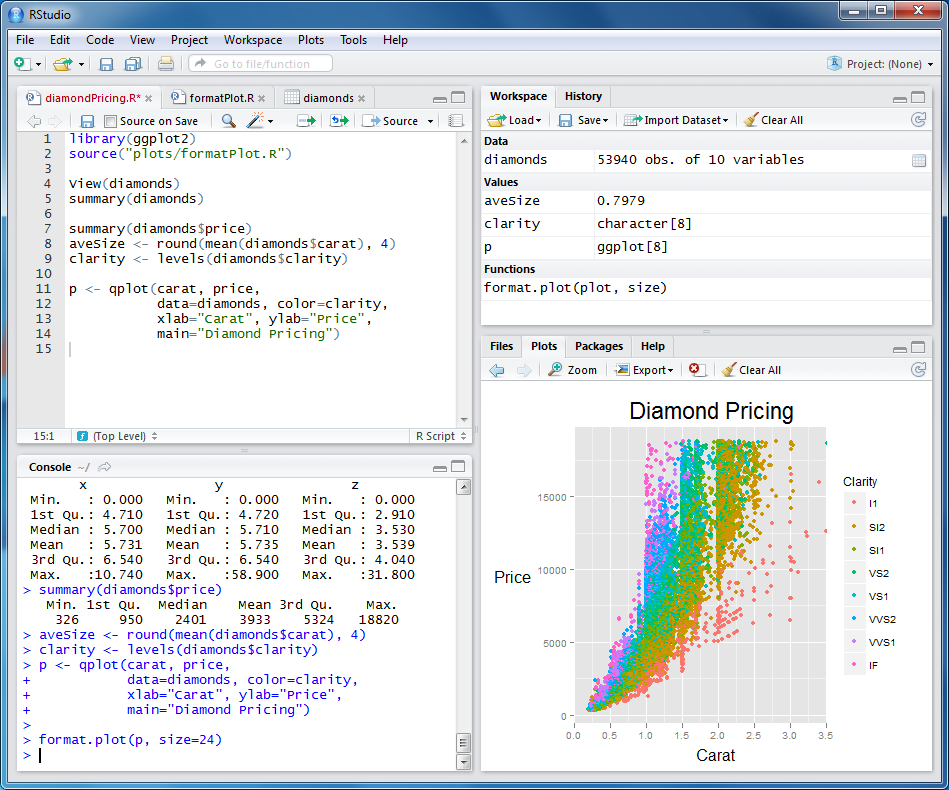
\includegraphics[width=1\textwidth]{drstudio-windows}
    \caption{RStudio's main window, courtesy of \url{https://www.rstudio.com}}
    \label{rstudiomainwindow}
\end{figure}

Clearly these are all advantages. Another advantage is that the code is not that different from what a Java or C programmer is used to writing, despite the language being very different in philosophy. A short snippet of R code that defines the product function can be seen in listing \ref{exampleRcode} and an example of filtering and substitution can be seen in listing \ref{exampleRsubstitution}, this example is particularly meaningful for R's capability to manipulate data sets (in the form of vectors, lists and data frames) in very concise ways.

\begin{listing}[h]
\begin{minted}{R}
f <- function(x, y) {
  r <- x * y
  return(r)
}
\end{minted}

\caption{Simple function definition in R}
\label{exampleRcode}
\end{listing}

\begin{listing}[h]
    \begin{minted}{R}
    # substitute negative values with 0
    values[values < 0] <- 0
    \end{minted}
    
    \caption{Example of value substitution and filtering in R}
    \label{exampleRsubstitution}
\end{listing}

The two down sides that I have found while working with R are the following:
\begin{enumerate}
    \item R's lists and vectors start at index 1, most other programming languages start the indexing at 0. While this is no technical shortcoming, it is a different mindset that one has to adapt to;
    \item The preferred assignment operator in R is "<-". Most of the time, while valid and totally interchangeable for simple assignments, the usage of "=" is discouraged. The usage of "=" for assigning default values for function parameters is preferable however \cite{RassignOps}.
\end{enumerate}

The multitude of tutorials and learning resources available on R online are making the programmer's life easier and make for a sweeter learning curve as the language is really popular in scientific internet circles it is easy to find answers to problems that arise while working with it. Also the plotting library ggplot2 \footnote{\url{https://ggplot2.tidyverse.org/}} is the state of the art in terms of drawing plots from code. While not very beginner friendly there are a lot of learning materials on the web for it and its documentation is plentiful to offset the learning curve of the library. The technical complexity of the library comes from the fact that the plots are very customizable.

\subsection{R alternatives}
As mentioned before, there are other alternatives to R, such as Python. While recently Python has seen an increase in usage \cite{pythongrowth}, its usefulness in scientific and statistical computing is still in development, and according to the cited article some developers switch from Python to R for data intensive tasks.

Both Python and R have the advantage of being fully open-source, that means that they are free for individual and commercial use. This fact also stands true for their big ecosystems of packages and libraries. There are also paid alternatives such as SAS \footnote{\url{https://www.sas.com/en_us/software/stat.html}} and SPSS \footnote{\url{https://www.ibm.com/analytics/spss-statistics-software}}. SAS, from the Graphical User Interface (or GUI, for short) point of view is very similar to RStudio (from which RStudio might have drawn some inspiration). SPSS is developed by IBM, so both of these seem like sound solutions for time-series forecasting, but have the disadvantage of being paid.

%TODO:space: expand on R and the ARIMA packges?

\section{Seasonal data} \label{seasonaldatasection}
In what is left of this chapter, I am going to explain each concept that I have used in understanding the ARIMA model and its variations, both in isolation and in relation to the model and its role in choosing the fittest ARIMA model.

I'm going to start with the concept of seasonality, which is an important one for longer time series, like I have here. As a reminder the time-series I'm going to inspect are 150 days long, with 288 observations every day.

Seasonality represents a concept similar to periodicity in mathematics, it's just named differently. In a nutshell it means that the values of a time series will repeat themselves season after season. The mathematical equivalent of this is exhibited in:
\[y_{t+m} \approx y_{t}\]
Where $ t $ is the time when the current observation is acquired and $ m $ is the period. For example if $ m $ is 24 hours, that means that the time series will repeat itself daily, meaning that every hour will be almost the same in regards to the same hour of the last day. For electricity consumption, one could say that the consumption for 12:00 PM will be similar to the demand of the 12th hour of the previous day, and the demand for the evening hour 20:00, will be the same or very similar to the consumption of the last day at 20:00.

Because seasonal patterns tend to be selected from a fixed set, one might try to create a classification of them \cite{hyndmanseasonalperiods}, which can be seen in table \ref{frequentSeasonalPeriods}.

\begin{table}[h]
\begin{tabular}{|c|c|}
    \hline 
    \textbf{Data seasonality} & \textbf{Seasonal period} \\ \hline 
    Annual & 1 \\ \hline 
    Quarterly & 4 \\ \hline 
    Monthly & 12 \\ \hline 
    Weekly & 52 \\ \hline 
\end{tabular} 
\centering
\caption{Frequently used seasonal periods}
\label{frequentSeasonalPeriods}
\end{table}

Data with a smaller seasonal period, such as weekly, daily, hourly, etc., may have multiple periods of interest. One might extract useful prediction patterns from daily data both at a weekly interval and a yearly one. For example in electricity demand prediction one can have daily periodicity in a week as well as monthly periodicity in a year, all for the same data. The patterns of consumption will repeat themselves for each morning, afternoon and evening, but also each month, compared to the previous years' same month, since some patterns occur in winter months and some other patterns occur in summer months. These monthly patterns are inclusive for the daily patterns, both coexist. Examples of such inclusive seasonal patterns are given in table \ref{multipleSeasonalPeriods}, also taken from \cite{hyndmanseasonalperiods}.

\begin{table}[h]
    \begin{tabular}{|c|c|c|c|c|c|}
        \hline 
        \textbf{Data seasonality} & \textbf{Minute} & \textbf{Hour} & \textbf{Day} & \textbf{Week} & \textbf{Year} \\ \hline 
        Daily & & & & 7 & 365.25 \\ \hline 
        Hourly & & & 24 & 168 & 8766 \\ \hline 
        Half-Hourly & & & 48 & 336 & 17532 \\ \hline 
        Minutes & & 60 & 1440 & 10080 & 525960 \\ \hline 
        Seconds & 60 & 3600 & 86400 & 604800 & 31557600 \\ \hline 
    \end{tabular} 
    \centering
    \caption{Higher seasonal periods that may include smaller periods}
    \label{multipleSeasonalPeriods}
\end{table}

For my data, which has been captured every 5 minutes, the seasonal periods are given in table \ref{5minSeasonalPeriods}.

\begin{table}[h]
    \begin{tabular}{|c|c|c|c|c|c|}
        \hline 
        \textbf{Data seasonality} & \textbf{Minute} & \textbf{Hour} & \textbf{Day} & \textbf{Week} & \textbf{Year} \\ \hline 
        5 minute & & 12 & 288 & 2016 & 105192 \\ \hline 
    \end{tabular} 
    \centering
    \caption{Seasonal periods for 5 minute data}
    \label{5minSeasonalPeriods}
\end{table}

Of course this might not always hold true because the value might not be exactly the same, this is one of the reasons I have used the $ \approx $ sign instead of a plain $ = $ in the previous equation. Another reason for using an approximation sign is that the seasonal period may not be exactly $ m $, or 24 hours in my example, since patterns may change with time, for example the lunch break from 12:00 may be shifted forward to 13:00 if the workplace demands it. The same with the evening example, if one has to run errands after work, one may arrive later than 20:00, hence the electrical energy consumption may see the pattern getting shifted. Some of the approximations are also given by the fact that years do not have the same number of days, hence the use of the 365.25 number of days in a year.

In order to capture different seasonal periods of a time series, multiple runs of the ARIMA algorithm are needed, in which the needed seasonality is used. In order to capture multiple seasonal periods at a time one might use Fourier terms. Depending on the number of Fourier terms included in the regression, the seasonal pattern may be smoother (for less terms) or more precise (for many terms). This concept will be further explained in the dedicated section \ref{dynamicharmonicregression}.

The usual way to find a time series' seasonality is to inspect two plots, namely:
\begin{enumerate}
    \item Seasonal plot: each data point is plotted against its respective season. An example plot may be seen in figure \ref{exampleseasonalplot};
    \item Subseries plot: each season is plotted separately, with data points collected in several mini time series plots. An example of such a plot may be seen in figure \ref{examplesubseriesplot}.
\end{enumerate}

As discussed in \cite{fpp2seasonalplot} and \cite{fpp2subseriesplot}, both of the above plots helps the statistician analyze a time series from the point of view of seasonality.
One has to start with inspecting a time plot of the data, in my case electricity consumption on the Y axis against time on the X axis. A time plot of the sub sampled at one hour intervals ph1 time series can be seen in figure \ref{exampletimeplot}. We can see that the plot starts at day 141 in our time series and ends at the beginning of day 148, hence I plotted 7 days worth of data.

\begin{figure}[h]
    \centering
    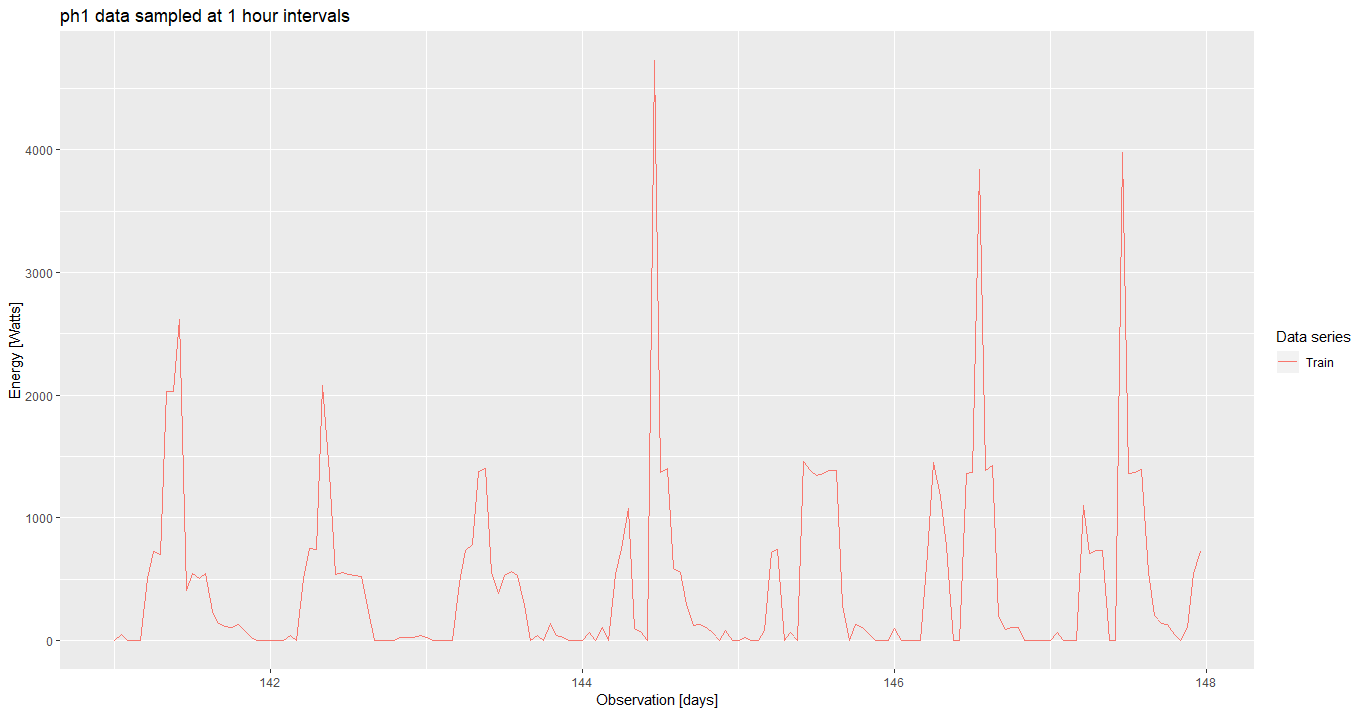
\includegraphics[width=0.75\textwidth]{d1hrsph1timeplot.png}
    \caption{Example time plot}
    \label{exampletimeplot}
\end{figure}

The seasonal plot, then takes this data and arranges it in hourly seasons, which is reflected on the X axis, which now has 24 points. This is in accordance with the fact that the data has been down sampled to 1 hour, the reason behind the down sampling being so we can better inspect the plot, by avoiding cluttering it. Because the original time plot contained seven days worth of data, in figure \ref{exampleseasonalplot} there are now seven time series each representing one day, with its respective seasons. The seasonality here becomes obvious in that each day observes an increase in electricity consumption after sunrise, starting with 05:00 in the AM, and ending around 20:00 in the evening.

\begin{figure}[h]
    \centering
    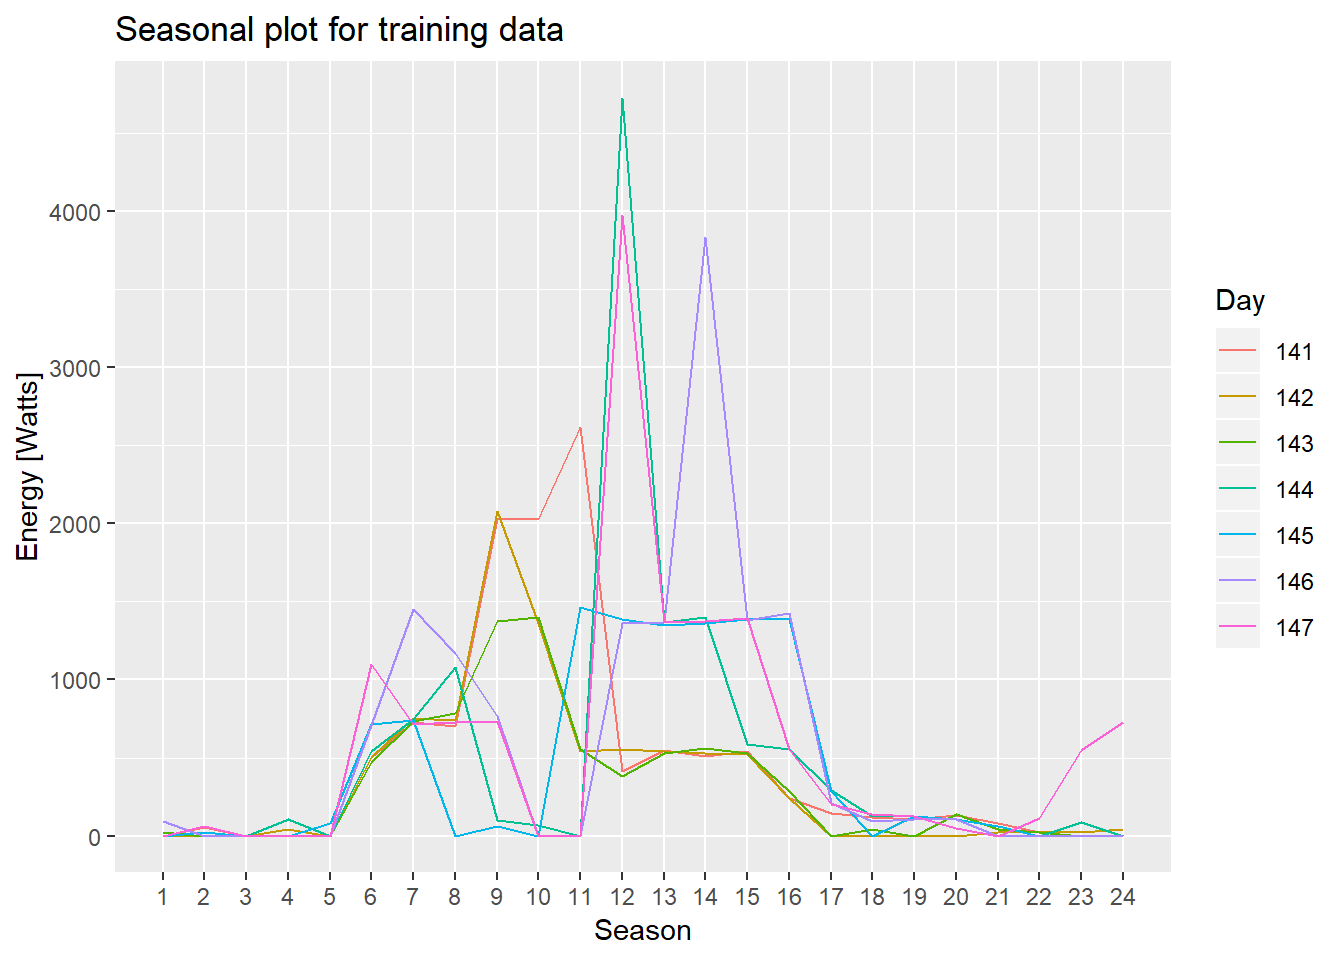
\includegraphics[width=0.75\textwidth]{d1hrsph1seasonalplot}
    \caption{Example seasonal plot}
    \label{exampleseasonalplot}
\end{figure}

The second type of plot that I'm concerned with is a seasonal sub series plot. Here, again, the original data in split into seasons, so the X axis also shows 24 points, because figure \ref{examplesubseriesplot} is a sub series plot of the same data presented in figure \ref{exampletimeplot}.
This time, though, each season is represented as a mini time series. The first observation of each day is arranged one after the other in the first mini series, then the second hour of each day is arranged in a mini series, and so on, completing all the 24 mini series representing each of the 24 seasons in a day. Because the original time plot had seven days worth of data, each mini time series now consists of seven points. The blue line for each series represents the mean of that series. From this plot, too, one can observe that the energy consumption values are increasing around midday. Hence concluding that we might have a daily seasonality, where electrical energy demand will repeat every 24 hours.

\begin{figure}[h]
    \centering
    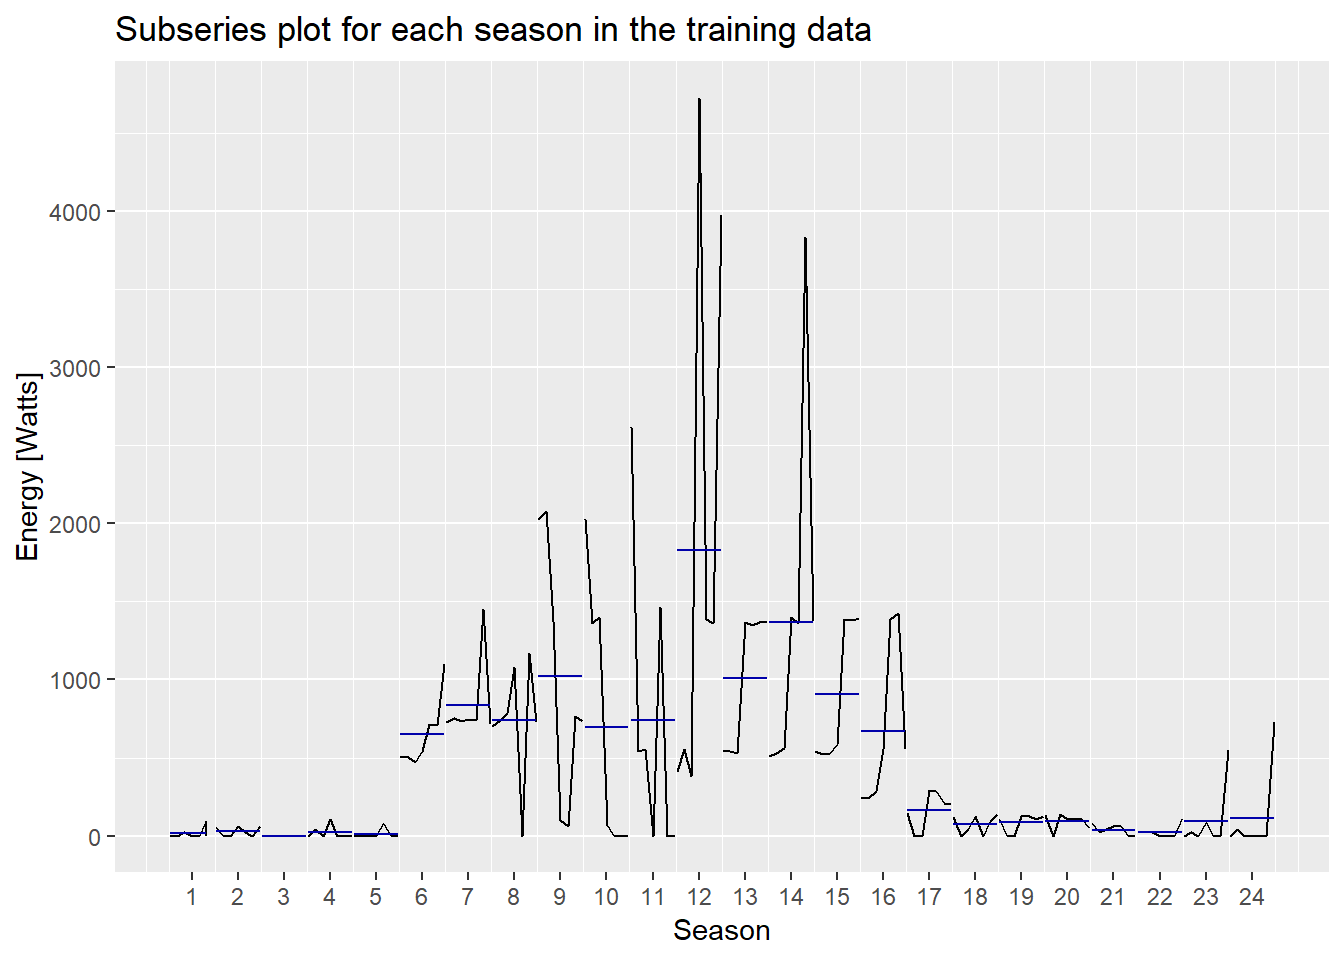
\includegraphics[width=0.75\textwidth]{d1hrsph1subseriesplot}
    \caption{Example subseries plot}
    \label{examplesubseriesplot}
\end{figure}

\subsection{Cyclic data}
The difference between seasonal data and cyclic data is that seasonality manifests itself at fixed intervals, annually, quarterly, monthly, weekly, etc. While cyclic patterns do not exhibit such predictable features, as they are not related to calendar events, but to economic and business conditions. Cyclic patterns exhibit much more volatile properties, the variations between cycles being wider and not as predictable as seasonal variations, which are more stable \cite{fpp2tspatterns}.

An example of cyclic data can be seen in figure \ref{dlynx}. Which shows the annual total of lynx trapped in the McKenzie River district of north-west Canada \cite{fpp2stationarity}.
\begin{figure}[h]
    \centering
    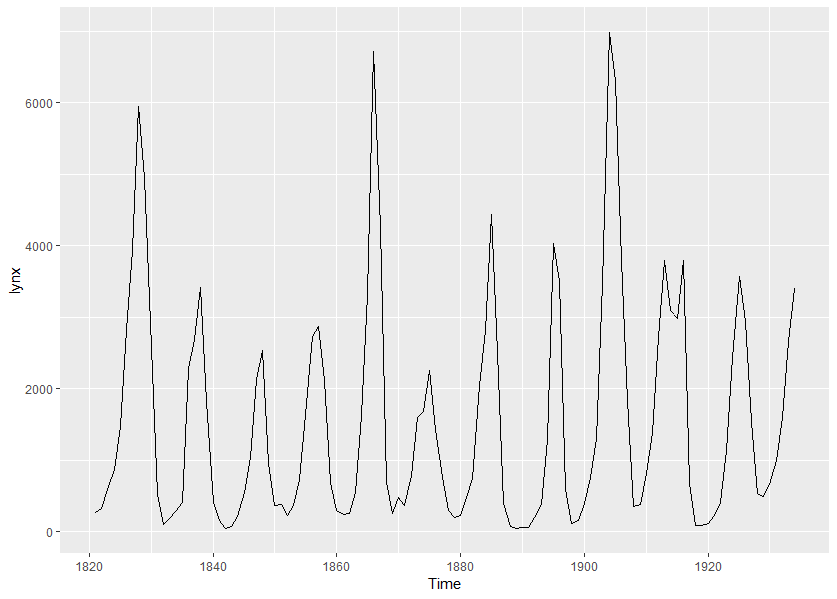
\includegraphics[width=0.75\textwidth]{dlynx}
    \caption{Example cyclic data}
    \label{dlynx}
\end{figure}

The cycles in the data are aperiodic and are caused when the population of lynxes increases and is too large to be able to feed, at that point they stop breeding and the population starts to decrease, after the regeneration of food sources, the population will, again, grow. After this point the cycle starts repeating, but with uncertainty with regards to each phase's length, making the time series cyclic, not seasonal \cite{fpp2stationarity}.

\section{Stationarity and non-stationarity}

Data stationarity is an assumption that is the basis of many time-series algorithms, including ARIMA. The ARIMA model need to be fed only stationary data in order to yield good results.

Data is said to be stationary when its statistical properties do not change regardless of the time window used to look at the data. This also means that statistical parameters of a time series, such as mean and variance, will be stable over time. \cite{fpp2stationarity}

What these statements lead to is that seasonal time-series are not stationary, their properties changing depending on which time they are observed at, if the season is different, so is, for example, the average electricity production from photo voltaic panels. If we look at summer data for electricity generation we might see that it is, on average, higher than in winter months. All because electricity production is favored by the sunny and non-cloudy days of summer, while in the winter electricity is not produced as much by photo voltaic panels since the sky is more often than not, overcast. Hence the winter electricity production should, on average, drop.

Other time-series that present increasing or decreasing trends, such as the data shown in figure \ref{energytrend} for the energy consumption plot are not stationary either. They are dependent on time, if we look at the data in different time slots, we're going to see, again, different means, depending on which years we choose to inspect.

One example of a stationary time series is a white noise series. Regardless of the time we choose to inspect the data, it will look much the same from a statistical standpoint. No noticeable changes happen that might influence the properties of the data. An example white-noise series is given in figure \ref{whitenoiseplot}. This figure was generated by the piece of R code given in listing \ref{Rwhitenoisecode}. This code generated 200 random points with an average of zero and a standard deviation of 1, plotted as if they were generated separately in time according to their generation index.

\begin{listing}[h]
    \begin{minted}{R}
    qplot(x=1:200, rnorm(200, mean = 0, sd = 1), geom='line') +
        ggtitle('White noise time-series') + 
        ylab('Random variable') + 
        xlab('Time')
    \end{minted}
    
    \caption{White noise plot code}
    \label{Rwhitenoisecode}
\end{listing}

\begin{figure}[h]
    \centering
    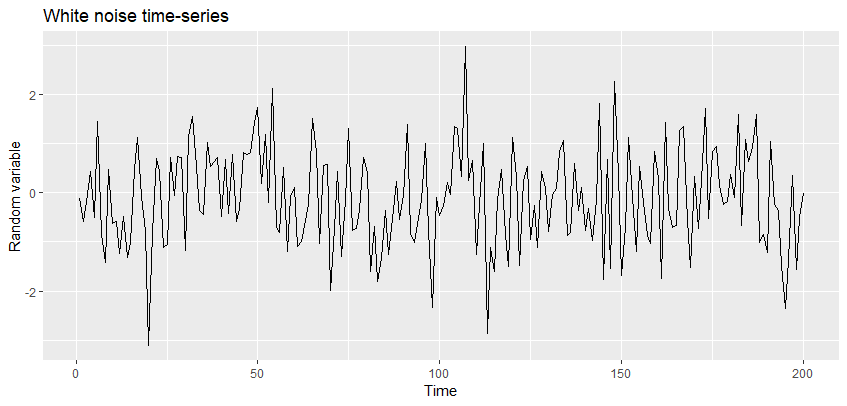
\includegraphics[width=0.75\textwidth]{dwhitenoise}
    \caption{White noise time-series}
    \label{whitenoiseplot}
\end{figure}

Of course not all time-series are random ones, so in order to be able to use them with ARIMA a kind of transformation has to be applied . This is the topic of sections \ref{differencing} and \ref{boxcoxtransformation}, making non-stationary data, stationary.

For the purpose of illustration I am going to present a few examples of non-stationary data sets from the \texttt{fpp2} R package \cite{fpp2stationarity} in figure \ref{nonstationarityexamples}.

% library("fpp2")
%grid.arrange(autoplot(goog200), autoplot(strikes), autoplot(elec), autoplot(beer), autoplot(eggs), autoplot(hsales), autoplot(pigs), nrow=4)
%
\begin{figure}[h]
    \centering
    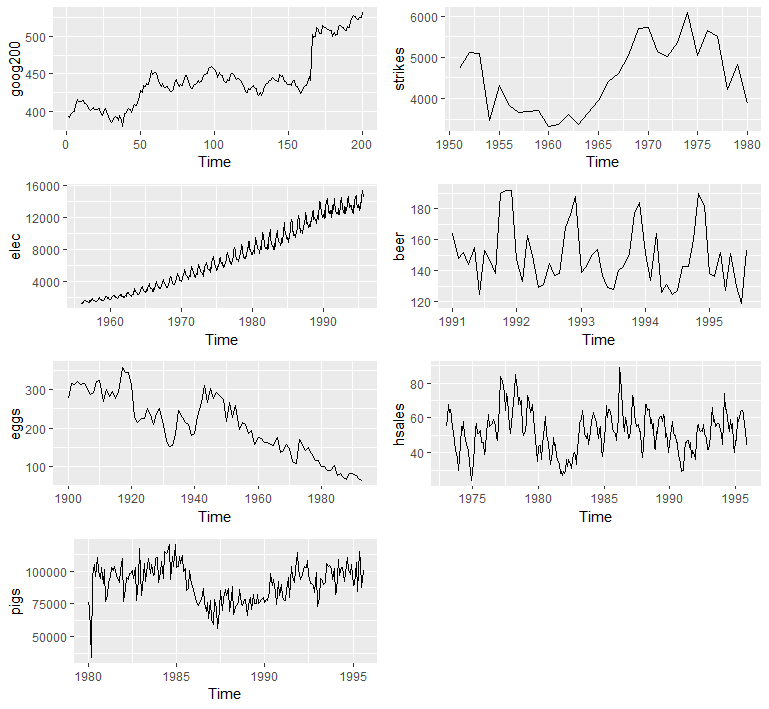
\includegraphics[width=0.75\textwidth]{dnonstationarityexamples}
    \caption{\texttt{goog200}: Google stock price for 200 consecutive days; \texttt{strikes}: Annual number of strikes in the US; \texttt{elec}: Monthly Australian electricity production; \texttt{beer}: Monthly Australian beer production; \texttt{eggs}: Annual price of a dozen eggs in the US (constant dollars); \texttt{hsales}: Monthly sales of new one-family houses sold in the US; \texttt{pigs}: Monthly total of pigs slaughtered in Victoria, Australia }
    \label{nonstationarityexamples}
\end{figure}

Series \texttt{elec}, \texttt{hsales} and \texttt{beer} are seasonal series, the same pattern is repeated over and over again across the plot. Then there are series \texttt{goog200}, \texttt{strikes}, \texttt{elec}, \texttt{eggs} and \texttt{pigs}, which also show trends or changing levels throughout the time they are observed. Increasing variance makes \texttt{elec} again non-stationary.

Apart from the graphical method presented here by inspecting the time series plots, there are also statistical tests that can determine whether a data set is stationary or not. One such test is the augmented Dickey–Fuller test (for short: ADF), which tests the null hypothesis that a given time-series is non-stationary. The result of the test is a negative number, the lower this number, that is toward $ - \infty $, the higher the chances that the null hypothesis should be rejected (ie. that the time-series under test is non-stationary with a given percentage of confidence). This test was developed by statisticians David Dickey and Wayne Fuller in 1979 \cite{adftest}. There are also alternative tests developed by other researchers on the same topic. Phillips–Perron test developed in 1986 \cite{unitroottestsPhillips} and the ADF-GLS test developed by Elliott, Rothenberg and Stock in 1996 are two such examples \cite{unitroottestselliott}.

\section{Differencing} \label{differencing}

In dealing with non-stationary data that must be made stationary one can use the concept of differencing, which is no different from the mathematical concept of differentiation, just applied to two observations of a time-series. \cite{boxjenkins}

The mathematical concept of differencing can be seen in equation \ref{differencingequation}.

\begin{equation}
y'_{t} = y_{t} - y_{t-1}
\label{differencingequation}
\end{equation}

Where $ y' $ represents the first difference of the $ y $ time-series. The first difference of a series is just the latest observation (that is, at time $ t $) minus the former observation (i.e.: at time $ t-1 $). For this reason, the differenced time series will only have $ n - 1 $ terms, given the fact that the original time-series had $ n $ terms, the explanation being that $ y'_{1} $ cannot be computed, since there is no observation before the beginning of time (when we started to observe the time series at $ t = 1 $). 

Intuitively the first difference of a variable models the change in that variable, think of the mathematical concept for the difference in positions, the result is the speed, or how fast the position of an object changes. The same way of thinking can be applied to electrical demand data, or any other time series, the first difference showing how the values of a measurement change, in our case, the change in electrical consumption from one data point to the other.

One can also represent second order differences if needed, or third order differences if the data requires such high order of differencing in order to become stationary. From a mathematical viewpoint second order differences look like equation \ref{2nddifferencingequation}.

\begin{equation}
\begin{split}
y"_{t} &= y'_{t} - y'_{t-1} \\
       &= (y_{t} - y_{t-1}) - (y_{t-1} - y_{t-2}) \\
       &= y_{t} - 2 y_{t-1} + y_{t-2} \\
\end{split}
\label{2nddifferencingequation}
\end{equation}

In the case of second order differences, the resulting time series will be $ n - 2 $ terms long. Intuitively, these second order differences model how the change in a variable changes \cite{fpp2stationarity}. Just as the mathematical counterpart does, if we differentiate the speed of an object, we get its acceleration.

Here lies the key for the "Integrated" part of Auto Regressive Integrated Moving Average algorithm. Above I specified that ARIMA should work only on stationary data, in fact this is true only or the ARMA algorithm, which cannot perform the differences that I presented in equations \ref{differencingequation} and \ref{2nddifferencingequation}. ARIMA on the other hand, through the $ I $ term, takes an integrated data series and differences it, making it stationary. Since differences are the exact opposite of integrations, this makes sense, ARIMA takes the integrated data, differences it, and theoretically speaking, feeds it later to the ARMA algorithm.

Because the standard way of looking at ARIMA is not in stages, ARIMA applies differences and then ARMA takes over and continues the computations, but as a whole, I'm going forward with the spoken and written convention
that ARIMA is applied to stationary data, although the data can be made stationary by ARIMA itself.

As explained in the section \ref{arimasubsection}, the $ d $ parameter of ARIMA controls how many differences are applied to the data. This is done under the notation $ I(d) $ and is performed by the statistician or researcher directly on the data.

Remember, the differencing operation's goal is to have data that looks as much as possible like white noise, by that I mean that it doesn't have features on the time plot that can be related to a specific time window.
I'm going to take the aforementioned data \texttt{goog200} and apply a single difference so that we can see the effect of such operation, the results can be seen in figure \ref{ddiffgoog200}.

% library("fpp2")
% grid.arrange(autoplot(goog200) + ggtitle("Original data"), autoplot(diff(goog200)) + ggtitle("First difference of the data") + ylab("goog200'"), nrow=2)
\begin{figure}[h]
    \centering
    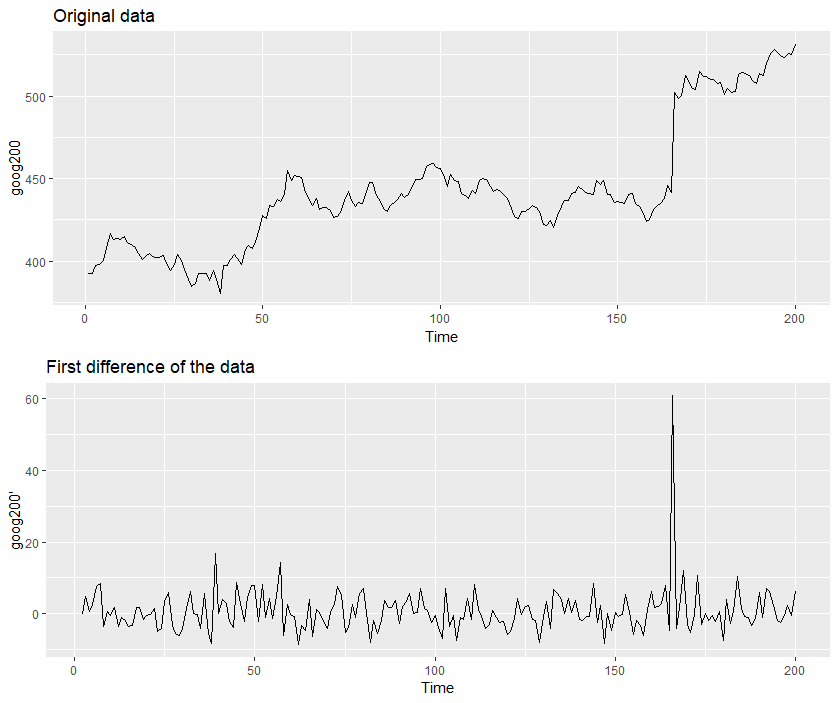
\includegraphics[width=0.75\textwidth]{ddiffgoog200}
    \caption{\texttt{goog200}: Google stock price for 200 consecutive days; \texttt{goog200'}: first difference of \texttt{goog200} data }
    \label{ddiffgoog200}
\end{figure}

The differenced data looks stationary, the first difference made obvious by the spike around day 165-166, where wee see a sudden increase in the level in the first plot, of the original data, and a spike in the differenced data, suggesting a big change from one data point to the next.

As noted in \cite{churvichunitroot} and \cite{nielsenunitroot} the notation $ I(d) $ comes from the fact that the process' characteristic equation that generated the given data has at least one unit root in the complex plane. Hence the tests mentioned earlier (for example: augmented Dickey-Fuller test) are in fact unit root tests and they check if such unit roots solve the process's characteristic equation.

\subsection{Seasonal differencing}

In dealing with seasonal data we employ seasonal differencing, which is very similar to non-seasonal differencing.
As noted in the section about SARIMA, the number of these seasonal differences will be denoted by the $ D $ parameter for the model.
Of course the seasonal differences will be applied only to seasonal data in order to make it stationary.

Mathematically speaking the equation for seasonal differences is given in equation \ref{seasonaldiffsequation}. Where $ m $ is the seasonal period.

\begin{equation}
y'_{t} = y_{t} - y_{t-m}
\label{seasonaldiffsequation}
\end{equation}

Again, using data from the \texttt{fpp2} R package, I'm going to illustrate the concept of seasonal differencing using the time series \texttt{euretail}, the European quarterly retail trade \cite{fpp2seasonalarima}. Being a quarterly measure, I expect that there is a need to apply at least a difference where $ D = 1 $ and $ m = 4 $ in order for the data to become stationary. As can be seen in figure \ref{euretaildiffs}, the first panel shows the unaltered, original, data. The second panel shows the seasonal difference, where $ D = 1 $ and $ m = 4 $, since there are four quarters in a year. Because the second panel is not clearly stationary, since there are trends in the data and a level shift towards the end, I have used another first difference, non-seasonal this time to make the data stationary. The non-seasonal difference was applied on the seasonally differenced data. The order in which the two differences are applied does not matter. Had I started with the first non-seasonal difference on the basis that the data has a trend, then applied the seasonal difference, the end result would have been the same. So if we were to apply the seasonal ARIMA model at this point, one would say it has the form: $ ARIMA(0, 1, 0)(0, 1, 0)[4] $, where $ d = 1 $, $ D = 1 $ and $ m = 4 $, I left the AR, MA, SAR and SMA terms empty by using $ 0 $ for placeholders.

%grid.arrange(autoplot(euretail) + ggtitle("Original data"), autoplot(diff(euretail, lag=4)) + ggtitle("Seasonal first difference of the data") + ylab("euretail, D=4"), autoplot(diff(diff(euretail, lag=4))) + ggtitle("First difference of the seasonally differenced data")+ ylab("euretail', D=4"), nrow=3)
\begin{figure}[h]
    \centering
    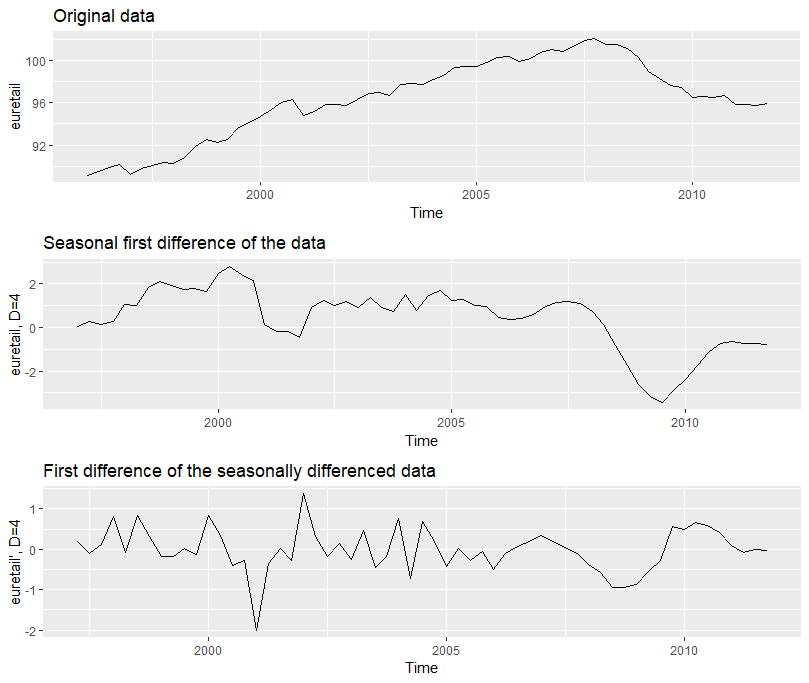
\includegraphics[width=0.75\textwidth]{deuretaildiffs}
    \caption{Quarterly retail trade index in the Euro area (17 countries), 1996–2011, covering wholesale and retail trade, and the repair of motor vehicles and motorcycles. With its seasonal and first non-seasonal differences applied.}
    \label{euretaildiffs}
\end{figure}

Please note that other seasonal period than $ m = 4 $ does not make sense here, considering the nature of the data (quarterly). The interpretation of such differences being that they represent the change from one season to the next, that is from one year's first semester to the next year's first semester, from one year's second semester to the next year's second semester, and so on.

In R one can use the \texttt{ndiffs} and \texttt{nsdiffs} functions from the \texttt{forecast} package in order to automatically determine the order of non-seasonal and seasonal differences needed to make a time series stationary. Both functions having support for multiple unit root tests, including the ones mentioned previously, ADF \cite{adftest} and PP \cite{unitroottestsPhillips}. I considered these functions when I investigated the electrical consumption and production data set used in this work, but I settled on the interpretation of the plots for choosing the order of differences.

\section{Box-Cox transformation} \label{boxcoxtransformation}

In figure \ref{nonstationarityexamples} I showed several examples of non-stationary data, among those time series resides the \texttt{elec} data series which because of its trend and increasing variance was categorized as non-stationary. When dealing with such data one might apply a transformation in order to be able to make the series stationary.

Examples of data transformations are given in \cite{fpp2transformations} and they include transformations such as:
\begin{itemize}
    \item Calendar transformations: used when examining monthly patterns, because the number of days in a month is different this analysis can become cumbersome, so the transformation entails transforming monthly values in daily average values;
    \item Population transformations: as is the case with calendar data, instead of analyzing data relative to the total, it might be easier to adjust the data per capita, thousand or million people;
    \item Inflation transformations: this adjustment is mostly used with economic data, where we have to adjust money value from a past period to the present, data for which inflation likely increased the value of objects;
    \item Logarithm transformations: logarithms have the property of making data interpretable relative to the original scale. If a base 10 logarithm is used, an increase of 1 in the transformed data will in fact be an increase of 10 in the original data set;
    \item Power transformations: power transformations such as square roots and cube roots may be used, but they are not as interpretable and suggestive as the other transformations mentioned here.
\end{itemize}

A set of adjustments that combines logarithms and power transformations, known under the name Box-Cox transformations, is defined mathematically as in equation \ref{boxcoxequation}.

\begin{equation}
w_t  =
\begin{cases}
\log(y_t)                     & \text{if $ \lambda = 0 $};  \\
\frac{y_t^\lambda-1}{\lambda} & \text{if $ \lambda \ne 0 $}.
\end{cases}
\label{boxcoxequation} 
\end{equation}

Where:
\begin{itemize}
    \item $ y_{t} $: is the original time series;
    \item $ w_{t} $: is the transformed time series;
    \item $ \lambda $: is a parameter of the transformation operation;    
    \item The logarithm is a natural one, that is, to base $ e $;
\end{itemize}

Some common cases of the Box-Cox transformation include setting $ \lambda = 0 $, in which case the natural logarithm transformation is used. While the other cases are power transformations, when $ \lambda \ne 0 $, together with some scaling by the same $ \lambda $ parameter. The only specific case of power transformations worth noting is when $ \lambda = 1 $, in this case the right hand side of the equation will become $ y_{t} - 1 $, thus accomplishing a simple downward shift with one unit.

For the above example of \texttt{elec} data, if we apply either a logarithmic transformation or a power one, the results will be satisfactory, as can be seen in figure \ref{boxcoxelec}, the variance is reduced in both cases. 

%grid.arrange(autoplot(elec), autoplot(BoxCox(elec, lambda=0)) + ylab(bquote("elec," ~ lambda ~ "=" ~ 0) ), autoplot(BoxCox(elec, lambda=0.26)) + ylab(bquote('elec,' ~ lambda ~ '=' ~ 0.26)), nrow=3)
\begin{figure}[h]
    \centering
    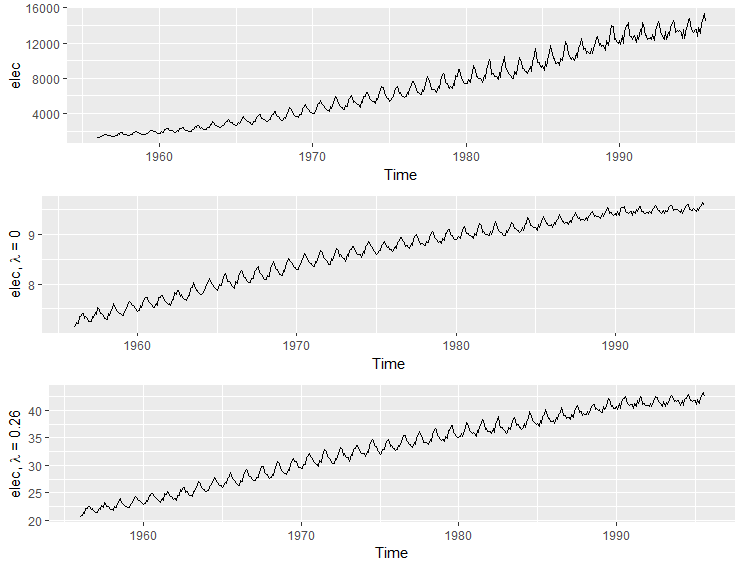
\includegraphics[width=0.75\textwidth]{dboxcoxelec}
    \caption{Top to bottom: \texttt{elec}: Monthly Australian electricity production; elec, $ \lambda = 0 $: logarithmically transformed \texttt{elec} data; \texttt{elec}, $ \lambda = 0.26 $: power transformed \texttt{elec} time series.}
    \label{boxcoxelec}
\end{figure}

I have applied a logarithmic transformation through a Box-Cox operation with the $ \lambda $ parameter set to $ 0 $. And a power transformation, again through a Box-Cox transformation with $ \lambda = 0.26 $. The value for $ \lambda$ has been generated using the \texttt{BoxCox.lambda} function from the \texttt{forecast} R package \cite{fpp2transformations} \cite{rforecastpackage}. One can easily see that the last two plots in figure \ref{boxcoxelec} have approximately the same height for the variations in the data, which is not true for the original data in the first plot from the figure.

Whenever transforming data and passing it to the ARIMA algorithm, the forecast data is still in the transformed space. So in order to get data in the original space back, we have to apply the inverse transformation \cite{fpp2transformations}, which in the case of Box-Cox is given by equation \ref{inverseboxcoxequation}.

\begin{equation}
y_{t} =
\begin{cases}
\exp(w_{t}) & \text{if $ \lambda = 0 $};\\
(\lambda w_t+1)^{1/\lambda} & \text{if $ \lambda \ne 0 $}.
\end{cases}
\label{inverseboxcoxequation}
\end{equation}

\section{Correlation of two variables}

If two variables $ a $ and $ b $ are correlated, that means that $ a $ influences $ b $ and vice versa. This could also mean that variables that are correlated might be redundant and half of them removed for the purposes of simplifying the model, since the information that one needs is already contained in the other half of the variables. When two variables are correlated, that means that if one increases, so will the second.

There is also the concept of anti-correlation, in this case when one variable goes up, the other goes down. One mathematical indicator for correlation is the Pearson Correlation Coefficient (or PCC for short) \cite{pearson1895note} developed by Karl Pearson, based on previous work by Francis Galton \cite{stiglercorrelationgalton}.

The Pearson Correlation for a data sample is presented mathematically in equation \ref{pearsonequation}.
\begin{equation}
r_{xy} = \frac{1}{n-1}\sum_{i=1}^{n}\left(\frac{x_{i}-\bar{x}}{s_{x}}\right)\left(\frac{y_{i}-\bar{y}}{s_{y}}\right)
\label{pearsonequation}
\end{equation}

Where:
\begin{itemize}
    \item $ x_{i} $: are the sample points for the $ x $ variable;
    \item $ y_{i} $: are the sample points for the $ y $ variable;
    \item $ n $: is the sample size for both variables;
    \item $ \bar{x} $, analogous for $ \bar{y} $: is the sample mean for the variable, defined as:
    \[\frac{1}{n}\sum_{i=1}^{n}x_{i}\]
    \item $ s_{x} $, analogous for $ s_{y} $: is defined as: 
    \[\sqrt{\frac{1}{n-1}\sum_{i=1}^{n}(x_{i}-\bar{x})^2}\]
    Also known as the sample standard deviation.
\end{itemize}
Please note that this formula for correlation may have many other forms, I chose the one easiest to understand on an intuitive level as explained in \cite{nauregression}, by Robert Nau from Duke University. 
$ r_{xy} $ may vary between -1 and 1. With a value of -1, the variables being anti-correlated, while at 1 being correlated, with the meaning given above: when one increases, so does the other in the case of correlation and when one increases the other decreases, in the case of anti-correlation. When $ r_{xy} \approx 0 $, then we say that the variables are not correlated, so we cannot assign a relationship between them since they are independent.

The explanation for the equation \ref{pearsonequation} is that $ r_{xy} $ should be positive if both variables $ x$ and $ y $ tend to vary on the same side of their means at the same point in time (that is if $ \left(\frac{x_{i}-\bar{x}}{s_{x}}\right) $ and $ \left(\frac{y_{i}-\bar{y}}{s_{y}}\right) $ have the same sign for the same $ i $) and $ r_{xy} $ should be negative if the variables vary on opposite sides of their means (that is, the standard scores have different signs)\cite{nauregression}.

\section{Autocorrelation function} \label{autocorrelationfunctionsection}

If one is interested in time-series, then one should look at the autocorrelation function.

The autocorrelation function computes the correlation between lagged values of the same time series. Lagged means: values at different points in time, that is, the correlation of the current observed value of the series with a previously observed value of the time series. Hence the name "autocorrelation", a correlation measure with oneself. Autocorrelation is also known as serial correlation.

It is computed by the equation given in \ref{acfequation} taken from "Forecasting: Principles and Practice" \cite{fpp2} which in turn uses Hyndman's previous research on the topic \cite{hyndman2015acf}.

\begin{equation}
r_{k} = \frac{\sum\limits_{t=k+1}^{n}(y_{t}-\bar{y})(y_{t-k}-\bar{y})}
{\sum\limits_{t=1}^{n}(y_{t}-\bar{y})^2},
\label{acfequation}
\end{equation}

This time I have used $ t $ instead of $ i $ to index the data, in order to make it more clear that now time-series are under the spotlight. The other notations have similar meaning as above. Note that $ r_{k} $ has a single letter as index since we're talking about the autocorrelation of a time series, I only have to specify an index, not two because the values are already in the time series for which we study the correlation. $ r_{1} $ measures the correlation between $ y_{t} $ and $ y_{t-1} $. $ r_{2} $ measures the correlation between $ y_{t} $ and $ y_{t-2} $ and so on. If I compute these coefficients on a time series, then I could also plot them, creating what is known as a correlogram. Two such plots can be seen in figure \ref{goog200acf}.

%grid.arrange(ggAcf(goog200) + ggtitle("goog200"), ggAcf(diff(goog200)) + ggtitle("goog200'"), nrow=2)
\begin{figure}[h]
    \centering
    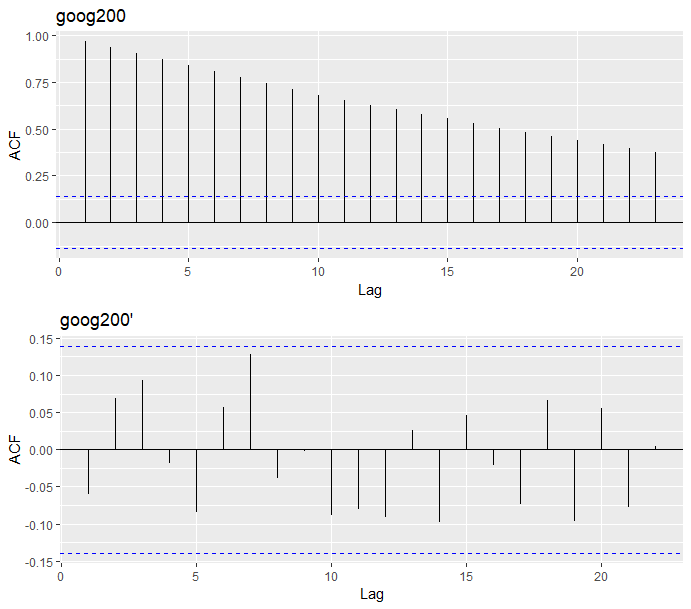
\includegraphics[width=0.75\textwidth]{dgoog200acf}
    \caption{Top: ACF of \texttt{goog200}; Bottom: ACF of the \texttt{goog200} first difference.}
    \label{goog200acf}
\end{figure}

One of the ways for identifying stationary or non-stationary time series is by using the autocorrelation function plot. This plot will drop to zero pretty quickly for a stationary time series, while on the other hand the ACF of non-stationary time series will decrease very slowly \cite{fpp2stationarity}. This is also how the augmented Dickey-Fuller test works at an intuitive level. Because the data are autocorrelated, future values may be created from past values, hence the data is non-stationary. An example of this behavior is also given in figure \ref{goog200acf}, where on the top plot we see the original \texttt{goog200} autocorrelation function and on the bottom plot of the figure we see the ACF of the differentiated series. The former is slowly decreasing towards zero since the data is non-stationary, while the other displays no such behavior since the differenced series is stationary.

\subsection{Critical values} \label{cirticalvaluesection}

The dotted blue lines in figure \ref{goog200acf} represent the critical values for the autocorrelation function (and later partial autocorrelation function). If the value of the ACF is between these lines, with a value close to zero, then the correlation is considered not significant, otherwise it is significant.

These significance values are usually considered at the 95\% interval for a two-tailed distribution. So by using a Z table, or standard normal distribution table, we can easily see that for a 95\% confidence interval corresponds a $ Z $ value of 1.96 ($ \approx 2 $).

The final confidence value is given by equation \ref{criticalvalueequation}
\begin{equation}
\bar{y} \pm Z \sigma 
\label{criticalvalueequation}
\end{equation}

Where:
\begin{itemize}
    \item $ \bar{y} $: is the mean of the sample data, in the case of Pearson correlation it is expected to be equal to 0;
    \item $ Z $: is the value taken from the standard normal distribution table for the necessary confidence interval, 1.96 for 95\% in the case at hand;
    \item $ \sigma $: the standard deviation of the data, in the case of normal distributions we expect it to be 1. We can replace this with the standard error of the mean: $ \frac{\sigma}{\sqrt{n}} $, which in turn is expected to be equal to $ \frac{1}{\sqrt{n}} $. Where $ n $ is the sample size.
\end{itemize}
So one could say that the critical values are approximately two standard deviations (or precisely 1.96) away from the mean. The final formula for computing the confidence values is: $ \pm \frac{1.96}{\sqrt{n}} $ \cite{nauregression}.  

\section{Partial Autocorrelation function}

The partial autocorrelation function (or PACF for short), is very similar to the autocorrelation function in a lot of ways \cite{boxjenkins}. The difference being that partial autocorrelation removes the influence of the middle lags and keeps the correlation of only the head and tail lags. That means that computing the partial autocorrelation of $ y_{t} $ and $ y_{t-k} $ will first remove the effects of lags $1, 2, 3, \dots, k-1 $. As a consequence of this is the fact that the first partial autocorrelation is the same as the first autocorrelation, since there is no other observation between the latest two \cite{fpp2nonseasonalarima}. What PACF accomplishes at an intuitive level is eliminating the possibility of $ y_{t} $ and $ y_{t-2} $ being correlated only because of the connection of the two with $ y_{t-1} $, which was clearly the case in ACF. Thus the PACF may uncover information related to both $ y_{t-2} $ and $ y_{t} $ that might be used for forecasting.

The critical values idea here is the same as for ACF, as explained in section \ref{cirticalvaluesection}.

\section{Choosing AR(p) and MA(q) terms} \label{choosingarandmasection}

For now I have only focused on the basic concepts that underlie the ARIMA model and that will help choose the right parameters for it.  I have only given indications on choosing the $ d $ parameter (the number of differences required to make the time series stationary) for the $ I(d) $ part of ARIMA.

I will now combine the two previous sections about autocorrelation function and partial autocorrelation function into what will be the guideline on how to choose the $ p $ and $ q $ parameters of ARIMA (and, of course, their seasonal counterparts $ P $ and $ Q $).

The ARIMA equation is given in \ref{boxjenkinsequation} and repeated here for clarity:
\begin{equation}
\tag{\ref{boxjenkinsequation}}
y'_{t} = c + \phi_{1}y'_{t-1} + \cdots + \phi_{p}y'_{t-p} + \theta_{1}\varepsilon_{t-1} + \cdots + \theta_{q}\varepsilon_{t-q} + \varepsilon_{t}
\end{equation}

As one can see, the auto regressive part of the equation, as the name implies, uses lagged values of the time series (possibly differenced, but for simplicity I will not consider that case in the explanation) scaled by some coefficients $ \phi_{1}, \phi_{2}, \dots, \phi_{p} $, the number of which will be chosen by the researcher, under the parameter $ p $. So the rule by which we should choose the number of AR terms in ARIMA is by inspecting both the ACF and PACF. 

It is clear that the ACF should display some kind of correlation between several terms since otherwise we couldn't exploit the relationship between lagged values in order to produce forecasts. But the question still remains, how many lagged values should we take into account for forecasting purposes? The answer to the question comes from the intuitive understanding of the PACF, namely: where do the lagged values stop being correlated with the current value of the time series? This is exactly the question that PACF answers, the lagged PACF value that is the last above the critical domain gives the number of observations that definitely influence (read: are correlated) with the current observation. In summary: if the ACF shows some correlation between lags, and the PACF at some point drops below the critical values we have a, so called, AR signature for which we choose $ p $ to be equal to the number of significant spikes in the PACF plot up to the point where they dip below the critical threshold of $ \pm \frac{1.96}{\sqrt{n}} $. In practice data will show either exponentially decreasing or sinusoidal ACF plots \cite{fpp2nonseasonalarima}.

%grid.arrange(autoplot(uschange[,"Consumption"]) + ylab("%") + ggtitle('Growth rates of personal consumption in the USA'), ggAcf(uschange[,"Consumption"]) + ggtitle(''), ggPacf(uschange[,"Consumption"]) + ggtitle(''), layout_matrix = rbind(c(1,1), c(2,3)))
\begin{figure}[h]
    \centering
    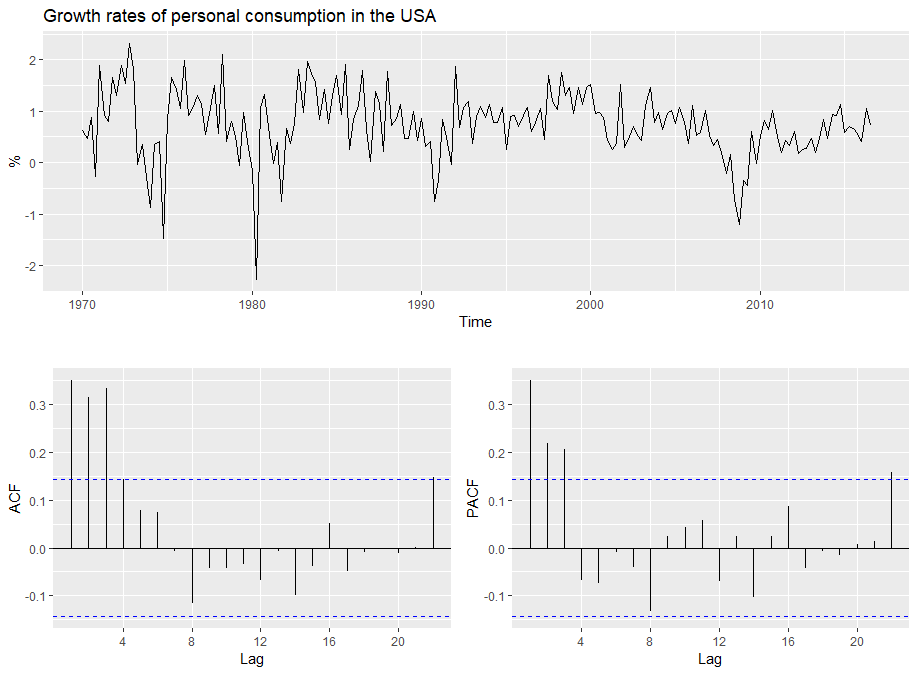
\includegraphics[width=0.75\textwidth]{duschangeacfpacf}
    \caption{Top, \texttt{uschange}: Percentage changes in quarterly personal consumption expenditure; Bottom left: ACF of \texttt{uschange}; Bottom right: PACF of the \texttt{uschange} data.}
    \label{uschangeacfpacf}
\end{figure}

Figure \ref{uschangeacfpacf} shows the \texttt{uschange} data from the \texttt{fpp2} R package \cite{fpp2} and its corresponding ACF and PACF plots. From this figure, using the rules listed above we may conclude that we have to set $ p = 3 $ since the ACF is an exponentially decaying function and the PACF shows three significant lags before becoming lower than the threshold. I have purposefully ignored the significant lag at the end of the PACF plot since we are working with 95\% confidence intervals. This means that we have 5\% chance of missing a significant spike in the plots. In concrete numbers that means 5 spikes in 100, or 1 in 20. Our plots show 22 lags, that means we can easily ignore one (or maybe miss one as an error) and still meet the requirement of 95\% confidence intervals.

Robert Nau also suggests, adding to the above rules, that positive ACF is also an indication of AR terms in the ARIMA model, that is of a need for using $ p > 0 $. \cite{nauarimaarmarules}

%grid.arrange(autoplot(usgdp) + xlab("Year") + ylab("US Dollars") + ggtitle('Quarterly US GDP'), ggAcf(usgdp %>% diff() %>% diff(lag=4)) + ggtitle('ACF after non-seasonal and seasonal differences'), ggPacf(usgdp %>% diff() %>% diff(lag=4)) + ggtitle('PACF after non-seasonal and seasonal differences'), layout_matrix = rbind(c(1,1), c(2,3)))
\begin{figure}[h]
    \centering
    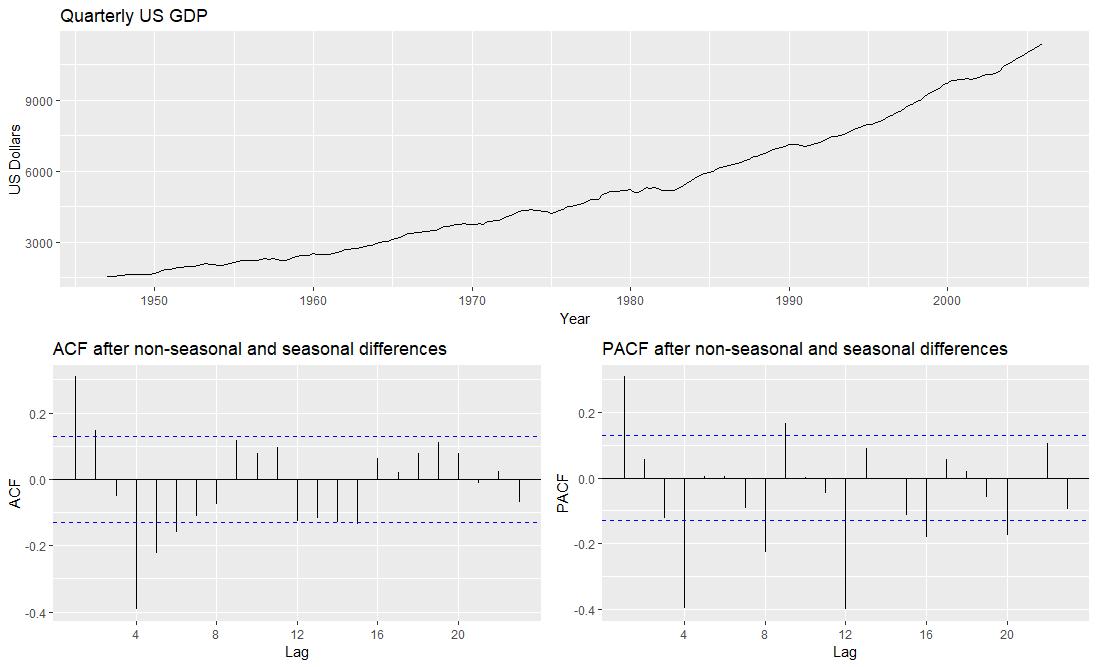
\includegraphics[width=0.9\textwidth]{dusgdpacfpacf}
    \caption{Top, \texttt{usgdp}: Quarterly US GDP; Bottom left: ACF of first non-seasonal and seasonally differenced \texttt{usgdp} data; Bottom right: PACF of first non-seasonal and seasonally differenced \texttt{usgdp} data.}
    \label{usgdpacfpacf}
\end{figure}

An example time series which yields a sinusoidal ACF after applying first seasonal and non-seasonal differences is presented in figure \ref{usgdpacfpacf}. For this data one might choose to set $ p = 1 $ since there is only a single lag significant in the PACF plot, while the other significant spikes are at seasonal lags, a topic which I will reiterate later on. \cite{hyndman2008forecasting}

According to Hyndman and Athanasopoulos, for choosing the $ MA(q) $ part of the model, one has to apply a similar reasoning, but swapped for the two plots. Here the $ q $ order will be chosen from the ACF plot, depending on the lag that becomes non-significant. At the same time the PACF plot should display sinusoidal features or exponential decaying shape \cite{fpp2nonseasonalarima}. Similarly for MA data, Robert Nau suggests, that negative (P)ACF is also an indication of MA terms in the ARIMA model. \cite{nauarimaarmarules}

As such, I may summarize the rules for choosing an $ ARIMA(p, d, 0) $ model as:
\begin{itemize}
    \item The autocorrelation function has sinusoidal form or is exponentially decreasing \cite{nauarimaarmarules};
    \item The partial autocorrelation function has significant lags up to an including lag $ p $, but none beyond it \cite{fpp2nonseasonalarima} .
\end{itemize}

While the summary of rules for choosing an $ ARIMA(0, d, q) $ process is:
\begin{itemize}
    \item The autocorrelation function has significant lags up to an including lag $ q $, but none beyond it;
    \item The partial autocorrelation function has sinusoidal form or is exponentially decreasing \cite{fpp2nonseasonalarima}.
\end{itemize}

In the same manner we shall decide on the $ SAR(P) $ and $ SMA(Q) $ parameters in the case of SARIMA for seasonal time-series. One such example might be the US GDP data presented in figure \ref{usgdpacfpacf}. In that figure, apart from the significant lags at the beginning of the series that determined the choosing of $ p = 1 $, we also see significant lags at and near index 4 for the ACF and at indexes 4, 8, 12, 16 and 20 in the PACF plot. These lags, at equal intervals of four suggest a seasonal term, and since we already used a non-seasonal AR term, we have to add a seasonal AR term in addition to that, thus leading to a final model of $ ARIMA(1, 1, 0)(1, 1, 0)[4] $. The $ p = 1 $ parameter was chosen using the above described rules, then $ P = 1 $ was chosen since we also have significant spikes at the seasonal intervals, which also determined the seasonal period of $ m = 4 $ because there are four quarters in a year. $ d $ and $ D $, representing the non-seasonal and seasonal differences, were set at 1 since I had to differentiate the data set once in order to make it stationary.

After the parameters have been chosen, the estimation of $ \phi $, $ \theta $, in case of ARIMA, and $ \Phi $, $ \Theta $ in case of SARIMA, is left to the algorithm. Usually the $ c $ constant in the ARIMA equation will be chosen as the mean of the data, remember though that this constant may not be included, depending on the software implementation of the ARIMA model.

%grid.arrange(autoplot(usgdp) + xlab("Year") + ylab("US Dollars") + ggtitle("Under-differenced data"), ggAcf(usgdp) + ggtitle(""), ggPacf(usgdp) + ggtitle(""), 
%autoplot(diff(usgdp)) + ylab("") + xlab("Year") + ggtitle("Autoregressive data"), ggAcf(diff(usgdp)) + ggtitle(""), ggPacf(diff(usgdp)) + ggtitle(""), 
%autoplot(diff(usgdp, differences=2)) + ylab("") + xlab("Year") + ggtitle("White Noise"), ggAcf(diff(usgdp, differences=2)) + ggtitle(""), ggPacf(diff(usgdp, differences=2)) + ggtitle(""),
%autoplot(diff(usgdp, differences=3)) + ylab("") + xlab("Year") + ggtitle("Moving average data"), ggAcf(diff(usgdp, differences=3)) + ggtitle(""), ggPacf(diff(usgdp, differences=3)) + ggtitle(""),
%autoplot(diff(usgdp, differences=4)) + ylab("") + xlab("Year") + ggtitle("Over-differenced data"), ggAcf(diff(usgdp, differences=4)) + ggtitle(""), ggPacf(diff(usgdp, differences=4)) + ggtitle(""),
%layout_matrix = cbind(c(1,2,3), c(4, 5,6), c(7, 8, 9), c(10, 11, 12), c(13, 14, 15)))
\begin{figure}[h]
    \centering
    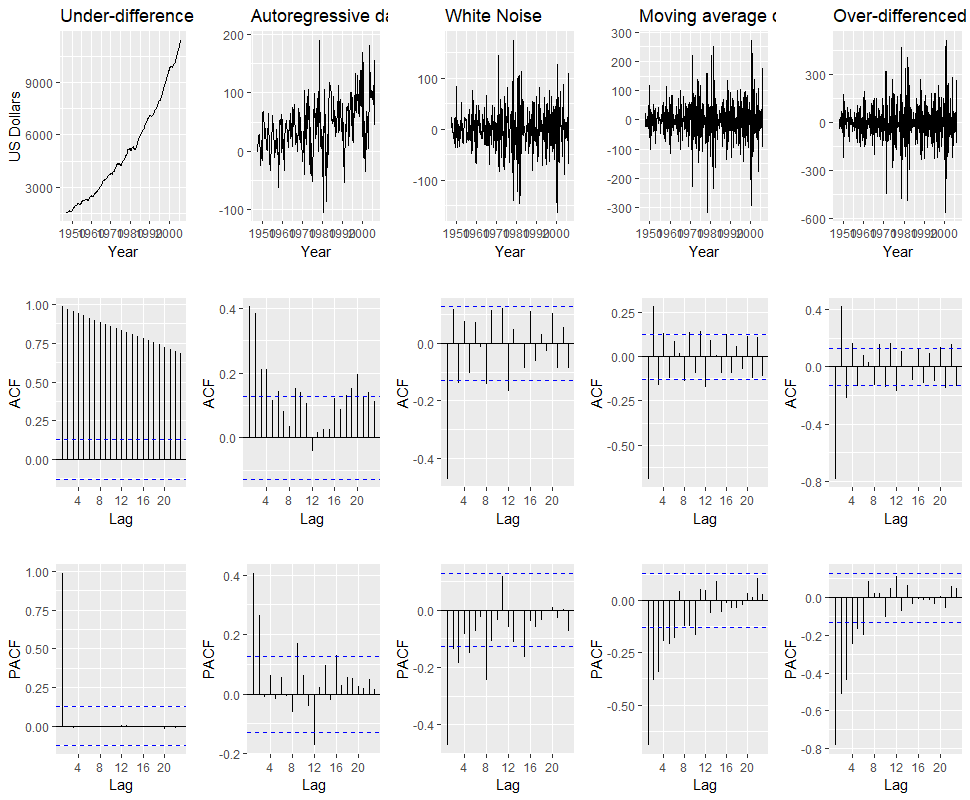
\includegraphics[width=1\textwidth]{darmadynamics}
    \caption{Top line, \texttt{usgdp} data (Quarterly US GDP), from left to right non-differenced data to over-differenced data; Middle line: ACF of the corresponding plots on the same column from the first line; Bottom line: PACF of the corresponding plots on the same column from the first line.}
    \label{armadynamics}
\end{figure}

In order to set things in perspective I have generated an image similar to "the autocorrelation spectrum", an image originally from Robert Nau of Duke University \cite{nauspectrum}. The image represents a grid of plots and can be seen in figure \ref{armadynamics}.

The top line represents the original data (first plot on the left) and then, going further to the right shows the data being sequentially differenced, an action that at first has the effect of making the time series stationary, then making it look like white noise, then over-differentiating it, making it look like data fit to be forecast using a moving average ARIMA model.

The middle line and the bottom line of the grid show the ACF and the PACF, respectively, of the first line of plots. If we consider the rules mentioned before, we can see that they apply nicely to these plots, the AR data being on the positive side of the (P)ACF plots and the MA data being on the negative side of these plots.

This also intuitively explains the choosing of MA and AR terms by swapping the ACF and PACF plots interpretation, since moving to the right of the plot moves from an AR process to an MA one, whereas moving from the right of the plot to its left moves between an MA process and an AR one. What this plot also shows is that the action of adding AR terms to an ARIMA model (that is: increasing $ p $) is almost equivalent to taking another difference of the time-series, while adding MA terms to an ARIMA model (that is: increasing $ q $) is almost equivalent to removing a difference \cite{nauarimaarmarules}.

\section{Residuals analysis}

Once the parameters for the model are chosen and the model is fitted on the data, one has to examine the produced errors. These errors, produced on the training set part of the data during the fitting process are called residuals \cite{boxjenkins}.

The residuals follow the equation \ref{residualsequation}.

\begin{equation}
e_{t} = y_{t}-\hat{y}_{t}
\label{residualsequation}
\end{equation}

Where:
\begin{itemize}
    \item $ e_{t}$: are the residuals;
    \item $ y_{t}$: are the observed values of the time series;
    \item $ \hat{y}_{t}$: are the fitted values from the model (the forecasts of the model for the training data).
\end{itemize}

If we extracted all useful information from the time series, then the produced residuals should not show any correlation and should have a mean of zero. Hence they should look like white noise. 

While fitting a model on the data I expect to extract all useful information from it, to take advantage of every correlation one can find between the lags of the time series, if this is not the case and information remains that I do not model, then this information will be visible in the residuals, through non-zero mean and correlation (like trends and level shifts). Also, according to Hyndman and Athanasopoulos, it would be useful if the residuals had constant variance and are normally distributed \cite{fpp2residuals}.

\begin{figure}[h]
    \centering
    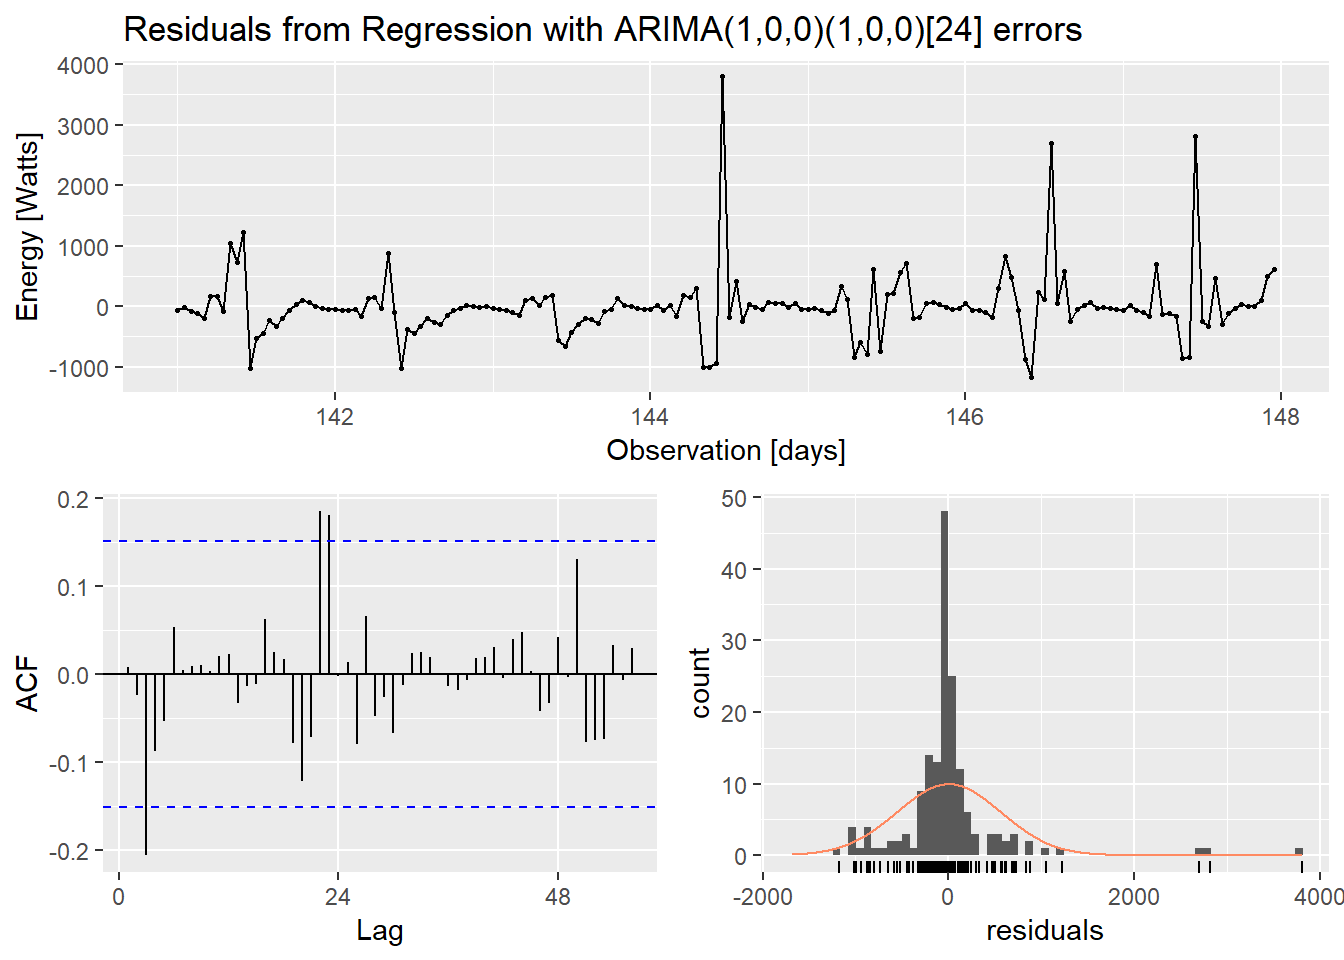
\includegraphics[width=0.75\textwidth]{d1hrsph1residuals-0eb37d71c48b26211c0dcb74b7712259}
    \caption{Top line, Residuals obtained after fitting an ARIMA model; Bottom line: ACF of the corresponding residuals (left) and their histogram on the right.}
    \label{1hrsph1residuals-0eb37d71c48b26211c0dcb74b7712259}
\end{figure}

For the reason presented above, I will analyze the residuals through several means, first of which being the plot shown in figure \ref{1hrsph1residuals-0eb37d71c48b26211c0dcb74b7712259}. This figure shows on the top plot the residuals obtained after fitting an ARIMA model to the data, this is a residuals versus time plot, in which we see that the residuals are indeed gravitating around mean zero and no significant trends or level shifts may be observed. In the lower left corner of the image is an ACF plot for the residuals, which, again looks relatively good, only three out of over fifty lags being significant, so we can safely ignore them and still be in the 95\% confidence interval. Finally, the lower right plot is a histogram plot of the residuals with the added guideline (in red) for a standard normal distribution for comparison purposes. I conclude from that plot that the residuals are as good as they can be, in reasonable limits, excluding only several outliers.
Another helping plot is the plot for the PACF of the residuals, which, again, should not show any correlation, for brevity purposes, such a plot is not shown here anymore, its structure not being different from an usual PACF plot.

\subsection{QQ plots}

If one has to compare a data set to a normal distribution, then a quantile-quantile plot comes in handy. A quantile is represented by the data point in a sorted data set under which reside a certain percent of the remaining data. Thus a quantile-quantile plot compares two data sets after computing their respective quantiles.

More often than not, in a QQ plot, one distribution is the standard distribution (the case also for the current work), but it can be used with other distributions as well. \cite{qqplots}

\begin{figure}[h]
    \centering
    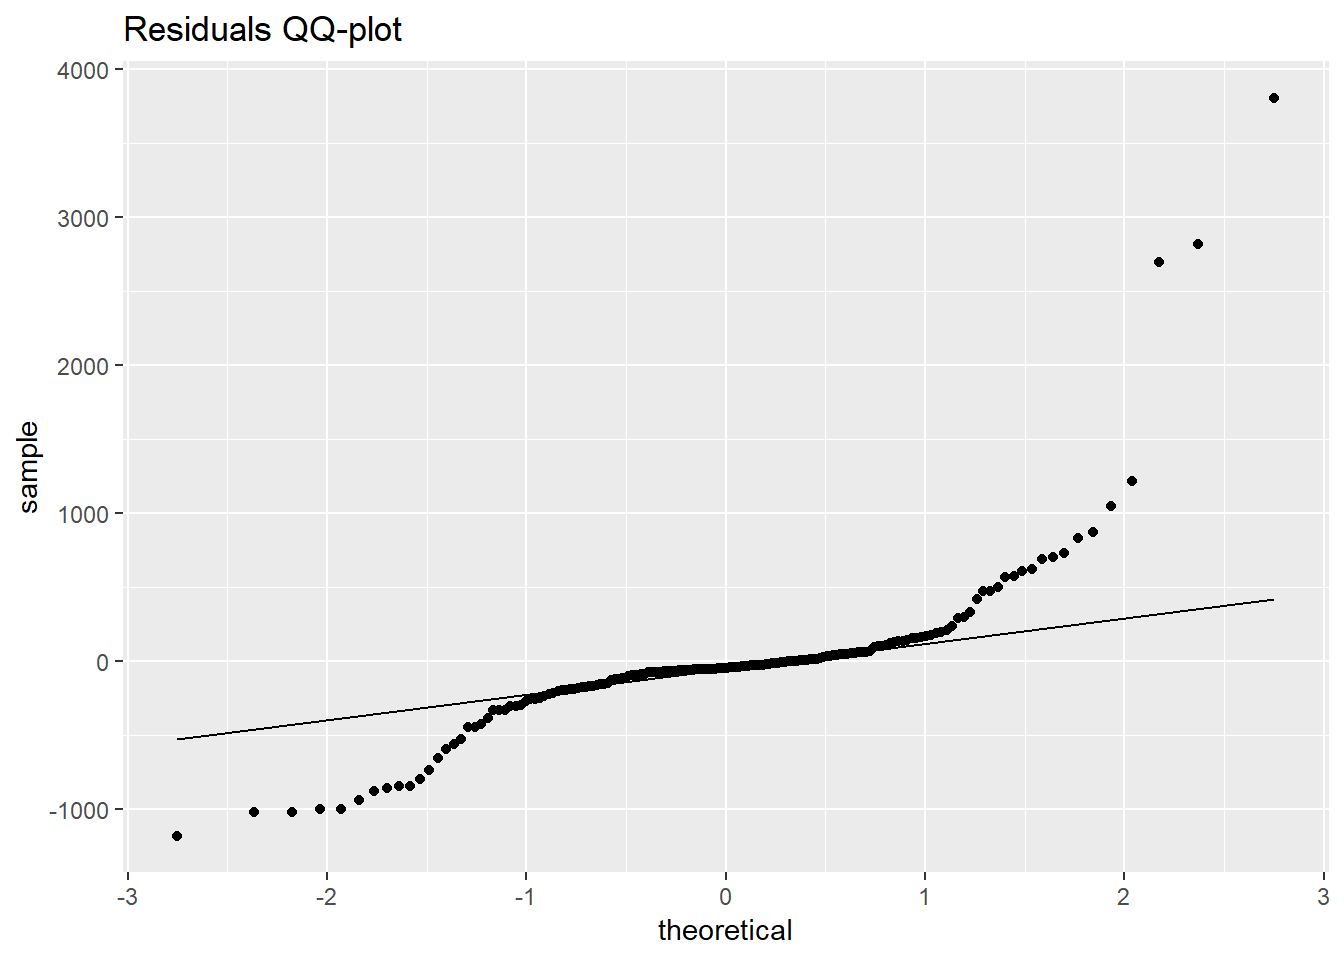
\includegraphics[width=0.75\textwidth]{d1hrsph1residualsqq-0eb37d71c48b26211c0dcb74b7712259}
    \caption{Example QQ plot.}
    \label{1hrsph1residualsqq-0eb37d71c48b26211c0dcb74b7712259}
\end{figure}

Figure \ref{1hrsph1residualsqq-0eb37d71c48b26211c0dcb74b7712259} depicts a QQ plot for a set of residuals obtained after applying ARIMA on a time series, the same residuals have been shown in figure \ref{1hrsph1residuals-0eb37d71c48b26211c0dcb74b7712259} as well. The black, straight, line represents an ideal standard normal distribution and the dots represent the quantiles of the residuals. Again, these residuals, are very close to a normal distribution, with the exception of three outliers in the upper right part of the plot, corresponding to the high values on the histogram plot presented in figure \ref{1hrsph1residuals-0eb37d71c48b26211c0dcb74b7712259}.

\subsection{Ljung-Box test} \label{ljungboxsection}

Apart from graphical interpretation of the plots, there are statistical tests for mathematically checking if the residuals have any autocorrelations left in them. The Ljung-Box test has been specifically developed for use with residuals generated by ARIMA models.

The test's equation is given in \ref{ljungboxequation}.
\begin{equation}
Q^* = n(n+2) \sum_{k=1}^h \frac{r_k^2}{n-k}
\label{ljungboxequation}
\end{equation}

Where:
\begin{itemize}
    \item $ n $: is the same size (total number of residuals);
    \item $ r_{k} $: is the sample autocorrelation at lag $ k $, see details in section \ref{autocorrelationfunctionsection};
    \item $ h $: is the number of residual lags being tested.
\end{itemize}

From Ljung-Box's formula we conclude that a higher $ Q^* $ will mean a more correlated set of residuals, hence I expect that the ARIMA model might be improved. This test statistic becomes helpful when comparing two ARIMA models by their residuals, a lower $ Q^* $ will mean less correlated residuals, hence a better model that extracts more of the information contained in the data. \cite{ljungboxtest}

%TODO:space:
%\section{Information criteria}
%
%Since I mentioned before that comparing ARIMA models can be done by how much information is left in the residuals (the autocorrelation of residuals, a measure indicated by the Ljung-Box test) I also have to mention that there are specific measures developed for the purpose of examining the fit of a model.
%
%Such measures include, but are not limited to \cite{fpp2predictors}:
%\begin{itemize}
%    \item 
%\end{itemize}
%
%But I will use out-of-band testing and the accuracy measures described in section \ref{accuracymeasuressection}.

\section{Accuracy measures} \label{accuracymeasuressection}

In order to be able to compare ARIMA models and how they fit the given time-series I have to measure how good a model performs on a data set.
This is done by measuring the forecasting errors a model makes.

Usually in computer science one measures the accuracy of a model by using the so called 80/20 rule \cite{8020rule}. This means that we randomly have to create two sets of data:

\begin{enumerate}
    \item The training set, accounting for 80\% of the total volume of data. The model will be ran on this part of the data set;
    \item The test set, accounting for the remaining 20\% of the data. The model's final evaluation will be done o this data set, no other changes to the model will be made to better fit the data in this set.
\end{enumerate}

The 80/20 rule may be bent a little bit, and the size of the training and test sets might be adjusted to a ratio of 60/40, 70/30 or 90/10, what is important is that we need two separate training and test sets.

In time-series analysis there is a catch to this rule, one cannot take a random sample from the data, since time-series are time dependent, shuffling the data points could potentially (and very probably) ruin the meaning of the data. So the way that I apply this rule is by sequentially using the first 80\% of the observations from the time-series for training and the rest for testing the models.

There are several measures used to judge the accuracy of a model, including \cite{Hyndman06anotherlook}:
\begin{itemize}
    \item Mean Error, is just the positive or negative average deviation from the true value, it is given by equation:
    \[\text{ME} = \frac{1}{n} \sum_{t=1}^{n} y_{t}-\hat{y}_{t}\]
    
    \item Mean Absolute Error, similar to the mean error, but always positive:
    \[\text{MAE} = \frac{1}{n} \sum_{t=1}^{n} |y_{t}-\hat{y}_{t}|\]
    
    \item Root Mean Squared Error, is the square root of the mean of square errors, according to: 
    \[\text{RMSE} = \sqrt{\frac{1}{n} \sum_{t=1}^{n} (y_{t}-\hat{y}_{t})^2}\]
\end{itemize}

Where:
\begin{itemize}
    \item $ n $: is the size of the test data;
    \item $ y_{t} $: is the real value from the test data;
    \item $ \hat{y}_{t} $: is the forecast value.
\end{itemize} 

A key difference between MAE and RMSE is the fact that the root mean squared error is more sensitive to outliers (because of the squared term in the errors) and hence some authors discourage its use \cite{armstrongevaluatingforecastingmethods}.

I will however, try to report all three exposed error measures in the practical part of this dizertation paper, while mainly using the mean absolute error for comparing and choosing the best models to use for a time series.
These error measures will be applied on the test set as a final means of comparison between models. According to their respective equations, the lower the errors, the better, so a low MAE and RMSE means a better performing model, while a lower ME doesn't necessarily mean a better model, here the closeness to zero matters, regardless of the negative or positive side.

%TODO:space: \section{The backshift operator}

\section{Dynamic harmonic regression} \label{dynamicharmonicregression}
When looking at electrical energy consumption and production we have to consider as well the seasonal aspect of data, since both the consumption and production are seasonally variable. Photo voltaic panels increase their production during sunny days in the summer months when the sky is clear, and have a reduced output during autumn and winter months.
According to Hyndman and Athanasopoulos \cite{fpp2dhr} long seasonal periods are better suited for dynamic harmonic regression. Seasonal ARIMA models (SARIMA) being a better match for short seasonal periods like 12 for monthly data and 4 for quarterly data.
The reason behind this being that daily data might be very noisy when looking at it in perspective, seasonal daily data for the yearly period literally means that the expected behavior for today is very similar to the one 365 days ago. This is a far fetched assumption because the seasonal pattern might change in a gap as big as the equivalent of one year.

Because of the reason exposed above, a dynamic harmonic regression might be employed to model longer seasonality periods. This means that the seasonal pattern is modeled using Fourier series and the remaining data, the so called errors, handled using ARIMA errors.

According to \cite{fpp2dhr} this approach is advantageous because:
\begin{itemize}
    \item Any seasonal period can be modeled;
    \item Different smoothness level for the seasonal patterns may be modeled depending on how many Fourier terms are used;
    \item The remaining, short-term dynamics of the time-series are easily captured with an ARMA model on the errors.
\end{itemize}

With the only down side that the seasonal period should not change, for example if one assumes a repeating seasonal period of 365 days, then dynamic harmonic regression will not be able to capture any change in this seasonal period, if it will become 360 or 370, no such change will be detected.

In the bigger picture of ARIMA, this dynamic harmonic regression is included in the ARIMAX model, ARIMA with exogenous regressors, a concept presented in section \ref{sarimaxsection}.

In order to use Fourier terms, we have to know how many of them to include, since closely mimicking a signal potentially requires one to include an infinite number of terms. Fortunately this is not the case, since we're only interested in capturing the seasonal patterns using Fourier terms. So for the purposes of this research, I have computationally varied the number of Fourier terms and selected the best performing model according to the minimum RMSE and MAE measures.

\section{Forecasting with dummies} \label{dummiessection}

Forecasting with dummies is similar to forecasting using Fourier terms. It's a regression with ARIMA errors, in other words ARIMAX, ARIMA with exogenous variables.

In the case of dummies, they model one-time events, for example public holidays, or some one-time public events, such as concerts or sporting events that take up several days and might influence electrical energy consumption or other time series that one might be interested in forecasting. Any event that doesn't fit into the "seasonal period" category can be modeled using dummies. Think of dummies as placeholders, they take on values only when a specific event has happened.

I will use seasonal dummies as an example, suppose each weekday consists of a separate event that repeats over and over again, then one needs to model weekdays separately as dummies. In the original ARIMAX equation (\ref{arimaxequation}), reiterated here for clarity:

\[
y'_{t} = c + \beta x_{t} + \phi_{1}y'_{t-1} + \cdots + \phi_{p}y'_{t-p} + \theta_{1}\varepsilon_{t-1} + \cdots + \theta_{q}\varepsilon_{t-q} + \varepsilon_{t} 
\tag{\ref{arimaxequation}}
\]

I have used only one external variable: $ x_{t} $. If one needs to model the seven days of the week, then one needs to use six dummy variables, that is: $ x_{1\dots6,t} $. The general rule being that one needs $ n - 1 $ dummy variables if there are $ n $ separate events to be modeled \cite{fpp2usefulpredictors}.

Each variable would only take two values, either zero or one, depending if the event has happened or is valid for a certain data point. For the weekday example the table \ref{weekdaydummies} depicts the way I have to choose the variables for a data set that has one observation per day.

\begin{table}[h]
    \begin{tabular}{|c|c|c|c|c|c|c|}
        \hline 
        \textbf{Week day} & \textbf{$x_{1,t}$} & \textbf{$x_{2,t}$} & \textbf{$x_{3,t}$} & \textbf{$x_{4,t}$} & \textbf{$x_{5,t}$} & \textbf{$x_{6,t}$} \\ \hline 
        Monday & 1 & 0 & 0 & 0 & 0 & 0 \\ \hline 
        Tuesday & 0 & 1 & 0 & 0 & 0 & 0 \\ \hline 
        Wednesday &	0 & 0 & 1 & 0 & 0 & 0 \\ \hline 
        Thursday & 0 & 0 & 0 & 1 & 0 & 0 \\ \hline 
        Friday & 0 & 0 & 0 & 0 & 1 & 0 \\ \hline 
        Saturday & 0 & 0 & 0 & 0 & 0 & 1 \\ \hline 
        Sunday & 0 & 0 & 0 & 0 & 0 & 0 \\ \hline 
        Monday & 1 & 0 & 0 & 0 & 0 & 0 \\ \hline 
    \end{tabular} 
    \centering
    \caption{Dummy variables for modeling week day events}
    \label{weekdaydummies}
\end{table}

Observe in table \ref{weekdaydummies} how Sunday is not represented by any value of one in the table, thus adhering to the $ n - 1 $ rule, having six variables for seven week day events. All the other week days have just a single 1 on their respective lines. For example Monday is modeled as $ x_{1,t} $, so each time we have an observation that was recorded on Mondays $ x_{1,t} $ will be 1, and 0 otherwise. These $ x_{1,t} = 1 $ will be repeated every 7 rows of the table (or observations), more generally $ x_{1,7t} = 1 $. The same applies for the other days of the week.

Using these variables the ARIMAX equation would become:

\[
y'_{t} = c + \beta_{1} x_{1,t} + \cdots + \beta_{6} x_{6,t} + \phi_{1}y'_{t-1} + \cdots + \phi_{p}y'_{t-p} + \theta_{1}\varepsilon_{t-1} + \cdots + \theta_{q}\varepsilon_{t-q} + \varepsilon_{t} 
\]

Thus giving weights (in the form of $ \beta_{1\dots6} $) to each week day whenever it is the case. This way, whenever the event takes place, a special emphasis will be made for the observation attached to the event. Similarly, when there is no event, all of $ x_{1\dots6,t} $ will be 0, so that there will be no special handling controlled by the coefficients.

In this manner one might encode as dummies weekends, hours of the day and other such periods or events, that might need special handling through dedicated coefficients (in the form of $ \beta_{1\dots6} $) in the ARIMAX polynomial.

\newpage
\chapter{Practical considerations}
This second chapter of the dissertation thesis will focus on the practical aspects of the work. More specifically the programming part and the methodological part as well as the results.

Basically I'm going to describe in more detail key concepts in my R code used for forecasting the time series in the data set.
More importantly, I'm going to describe the methodology or how I applied the theoretical knowledge to forecast the data. The abstract steps and concepts described in the first part of this paper will now become concrete actions that will lead to choosing an ARIMA model and using it for forecasting time series.

The practical considerations are of importance because, according to Moore's law \cite{moore:1965} computing power is still increasing. 
With the trend of embedded devices being more and more inter-connected in the IoT concept (internet of things) we can expect the forecasting algorithms to be present in such devices as well and to be able to influence and to give indications on our electrical energy consumption behaviors.

One such application might be in photo voltaic panels. A next-generation appliance that allows the home owners to have real-time data regarding the electrical energy production patterns of their photo voltaic panels. Like all "smart" devices, it may have downsides, like security vulnerabilities, but its pros outweigh the cons. These "smart" capabilities are enhanced by the increasing computational power of embedded devices, through which operations like consumption and production of electrical energy forecasting for a house may be made.

This paper doesn't aim to give insight on how to implement forecasting algorithms in embedded devices, but can be used to draw conclusions of what is possible and what is not possible with regards to complex forecasting algorithms such as ARIMA.

\section{Applied R}

In this section I'm going to present key pieces of code from the work I have done to forecast electrical energy consumption and production using the ARIMA model and the R programming language.

As presented in section \ref{rtheorysection} I have chosen to work with R after some very low-productivity work I have done with Java in a similar fashion. R, through its design, centered on quick feedback by its Read-Eval-Print-Loop philosophy, enables the programmer to easily and immediately see the results of the code he is writing. There is no need for a compilation and running step, both of which happen at the same time. While running depends on quality of the written code and what it does, compilation on the other hand is almost instantaneous, and transparent to the user.
This is a consequence to the fact that R is in fact belonging to the scripting languages family. 

R also benefits of a very large collection of packages, it has over 13000 (thirteen thousand) of them available online\footnote{Early 2019, according to: \url{https://cran.r-project.org/web/packages/}}. These packages vary in function and cover a wide range of scientific fields, there are packages that can be used to accomplish different tasks, from simple string operations, to what I need for this paper: forecasting of time-series data.

The main packages I am using are: 
\begin{itemize}
    \item \texttt{forecast}: The forecast package is the basis of this work since it provides the ARIMA model implementation that I'm using. It offers all the forms of ARIMA a statistician might need, from simple ARMA, to ARIMA and (S)ARIMAX. It is based on the work of Rob J. Hyndman, a highly active and productive professor of statistics at Monash University in Australia \cite{forecastpackagearticle} \cite{forecastpackagemanual}. Using this package requires one to understand at least the meaning of the algorithms' parameters;
    \item \texttt{ggplot2}\footnote{\url{https://ggplot2.tidyverse.org/}}: This may be the most popular package in the scientific world of R since it easily allows the programmer to display plots of data. Its variety of plots make it suitable to every scenario imaginable while also staying very flexible and customizable. It implements a very modular way of building the plots, based on the book The Grammar of Graphics \cite{thegrammarofgraphics};
    \item \texttt{tictoc}\footnote{\url{https://cran.r-project.org/package=tictoc}}: A small and simple package that allows one to measure how much time a piece of code takes to run;
    \item \texttt{foreach}\footnote{\url{https://cran.r-project.org/package=foreach}} \& \texttt{doParallel}\footnote{\url{https://cran.r-project.org/package=doParallel}}: These two packages, used in conjunction, allow the programmer to easily write parallel R code.
\end{itemize}

The functions that I used from the \texttt{forecast} package will be described in detail in section \ref{forecastpackagesection}.

The package \texttt{tictoc} mainly consists of functions \texttt{tic()}, called when timing of a code section should begin and \texttt{toc()}, called when timing of a code section should end. The last call has the side effect of printing the time elapsed between the \texttt{tic()} and the \texttt{toc()} call, this behavior can be avoided and the time elapsed could be stored in a variable for later processing.

The \texttt{ggplot2} package offers a wide range of plots that one can create with several simple lines of code. All plots in this work have been created using features of \texttt{ggplot2}. From displaying simple time plots of time-series data, seasonal and seasonal sub-series plots to the QQ plots used in analyzing the residuals, \texttt{ggplot2} offers this functionality, allowing the programmer to focus on more important things like finding model parameters, instead of manually creating plots. If this package wouldn't have existed the programmer himself should have arranged the data in sub-series and then plotted them together in a seasonal sub-series image, an operation that is time consuming and not really focused on the end-goal of the project.

Fortunately there is this package that automates much of the tasks needed for creating different kind of plots from time-series:

\begin{itemize}
    \item \texttt{ggseasonplot}: Plots like the one in figure \ref{exampleseasonalplot} are easily constructed by using the \texttt{ggseasonplot()} function of the \texttt{ggplot2} library;
    \item \texttt{ggsubseriesplot}: In order to avoid manually computing each subseries of a time-series one can use the \texttt{ggsubseriesplot()} function offered by \texttt{ggplot2} to compute the subseries and plot them, along with their respective mean values, thus saving the programmer some time, an example plot produced by this function can be seen in figure \ref{examplesubseriesplot};
    \item \texttt{ggAcf} and \texttt{ggPacf}: While R offers functions to compute the numerical values of the (partial) auto correlation function, this will directly plot the numerical values together with the 95\% critical value, examples of both of these plots can be seen in figure \ref{uschangeacfpacf}.
\end{itemize}

The QQ plot can be drawn easily using the code in listing \ref{qqplotr}. In this listing the \texttt{residuals} variable represents the vector of residuals obtained after fitting the ARIMA algorithm on the data.

\begin{listing}[h]
    \begin{minted}{R}
    
    ggplot(data.frame(y=residuals), aes(sample=y)) +
        stat_qq() +
        stat_qq_line() +
        ggtitle('Residuals QQ-plot')
    
    \end{minted}
    
    \caption{Drawing a QQ plot in R}
    \label{qqplotr}
\end{listing}

Another package that I have used in developing this project is the \texttt{doParallel} package. This package, according to their description \footnote{https://cran.r-project.org/web/packages/doParallel/index.html}, allows the programmer to easily parallelize a piece of code by using the \texttt{\%dopar\%} function when iterating over a collection of data. In other words, this package transforms the usual (sequential) \texttt{foreach} loop in a parallel loop. Of course this can only be done if the data are independent from each other and if the processing of the data doesn't depend on previously computed results. For ARIMA and time series both of these assumptions hold true. The listing \ref{exampleparallelcode} shows an example on how the \texttt{doParallel} package can be used practically and demonstrates another reason for using R in the scientific community, the ease of use of such packages improve the life of the programmer. In listing \ref{exampleparallelcode}, the square root function will be run in parallel, thus computing all results at once\footnote{given the fact that the computer where the code is run has more than 3 cores}.

\begin{listing}[h]
    \begin{minted}{R}
    
    foreach(i=1:3) %dopar% sqrt(i)    
    
    \end{minted}
    
    \caption{Basic usage of the \texttt{doParallel} package}
    \label{exampleparallelcode}
\end{listing}

The package also provides settings for the number of cores to be used when parallelizing code, but these are omitted here for relevance issues.

\subsection{The forecast package} \label{forecastpackagesection}

The main R package leveraged by this dissertation is the \texttt{forecast} package \cite{forecastpackagemanual}, written by Rob J. Hyndman and others \cite{forecastpackagearticle} this is the main package used when forecasting time series.
Combined with the time series data type in R (\texttt{ts()}) it provides the widest range of possibilities for analyzing and forecasting such data.

Compared with other solutions in other programming languages this package is used and maintained by professionals which conduct their work and research that requires forecasting tools. Hence we can be sure of the quality of the tools we are using.

In R (and consequently in the \texttt{forecast} package) there is a small particularity that the reader should be aware of: the term frequency doesn't have its meaning from physics, but it means in fact the seasonality of the data \cite{hyndmanseasonalperiods}.
For example if we have have seasonal data with a period of 12, which corresponds to monthly data, then in R we would specify a frequency of 12.
This is just a notation mishap and once noted it is unlikely to cause confusion, so I advise the reader to stay alert since, depending on the context, I may use the term "frequency" to mean the seasonal period of the data.

The most notable functions in the R \texttt{forecast} package are:
\begin{itemize}
    \item \texttt{Arima}: This function implements the ARIMA model in all its presented forms. It accepts two sets of parameters, one for the non-seasonal part and one for the seasonal part, and a seasonal period for the data, as well as the data to be predicted. Optionally, the programmer may specify external regressors as well if dummies or Fourier terms are to be used. The return value of this function is a model which can later be used to produce forecasts;
    \item \texttt{forecast}: The \texttt{forecast} function accepts a model and a number of observations for which to produce predictions. It uses the model to generate the requested number of forecasts;
    \item \texttt{fourier}: This is a helper method used to generate a matrix of Fourier terms used as the external regressors in the \texttt{Arima} function;
    \item \texttt{BoxCox} and \texttt{InvBoxCox}: Computes the BoxCox transformation (and its inverse) for a given "lambda" ($ \lambda $) parameter and data set.
\end{itemize}

As we see from the functions presented above, the model fitting to data is done by the \texttt{Arima} function and the predictions are computed using the \texttt{forecast} function (which is a homonym to the package's name). These two are the main steps of the methodology I applied in forecasting the electricity consumption and production, which is presented in detail in section \ref{methodologysection}. The two functions or steps in the methodology are somewhat equivalent to the "training" and "evaluation" terminology from the domain of neural networks for example.

%TODO:space
%\subsection{Benchmark methods in code}
%Show meanf, average, naive code.

\subsection{ARIMA in code} \label{arimaincode}
The code for calling the \texttt{Arima} function for building a model and creating predictions is presented in listing \ref{examplearimacode}.

\begin{listing}[h]
    \begin{minted}{R}
    fit <- Arima(data, order=c(1, 0, 0), xreg=fourier(data, K=2))
    predictions <- forecast(fit, h=h, xreg=fourier(data, h=h, K=2))
    \end{minted}
    
    \caption{Model fitting and forecasting using the \texttt{Arima} function of the \texttt{forecast} R package}
    \label{examplearimacode}
\end{listing}

This listing, while short, uses most of the concepts presented until now and sums up the usage of the \texttt{forecast} package.
First, the data is fitted using an $ ARIMA(1, 0, 0) $ model with seasonality modeled by external regressors in the form of second order Fourier terms. The data may be optionally split using the 80/20 Pareto rule for training and test data. The \texttt{fourier} function automatically generated the proper number of Fourier $ sin $ and $ cos $ pairs according to the length of the data.

The second part of the listing involves actually using the fitted data to create predictions. The return value of the \texttt{forecast} function is an object of class \texttt{forecast} (in an object oriented language, which R actually is). This object has several members, including a \texttt{mean} member, that stores the actual predictions of the algorithm. These are called "point predictions" since they give the actual value we might expect the data to take.

The \texttt{h} parameter represents the number of observations that we want to predict. We also have to specify the external regressors that should be used when predicting the data. Since the regressors were included in the initial model fitting, we also have to provide them now in order for the model to work, otherwise predictions cannot be made due to missing data.

This is a down-side of using external regressors, they have to be available for the future data at the time of forecasting, which if we'd like to use an organic value (such as temperature) to help predict other time-series creates a chicken and egg type of problem. Suppose we'd like to forecast energy consumption based on the temperature outside. This can only be done if the outside temperature is available before the electricity is actually consumed. Although one can indeed forecast the temperature first and then forecast the electricity consumption, this is not feasible since it involves two layers of forecasting and, consequently, two opportunities for errors to accumulate. This is the reason I have chosen to work with Fourier terms and dummy values for the external regressors fed into the ARIMA model. Both of them can be artificially created based on past data, cleanly solving the chicken and egg problem and avoiding accumulating errors while forecasting.

In order for the forecasts to be accurate, I have heeded the advice given by Hyndman in \cite{fpp2dhr} to vary the order of the Fourier terms dynamically in order to find the best matching one.

Actual code for this can be seen in listing \ref{actualKcode}.

\begin{listing}[h]
\begin{minted}{R}

    best.fcast.k.1hrsPh1 <- NULL
    best.k <- 0
    #K must be not be greater than period/2
    for(k in 1:(frequency(datasets[['1hrs ph1']]$series)/2))
    {
        print(paste("Trying k =", k))
        m <- paste0('Arima(order=c(1, 0, 0),
            seasonal=c(1, 0, 0),
            xreg=fourier(., K=', k, '))')
        xreg <- paste0('fourier(., h=h, K=', k, ')')
        current <- fullforecast(model = m,
            dataset = datasets[['1hrs ph1']]$series,
            transformation = 'identity()',
            traindays = best.traindays,
            testdays = best.testdays,
            xreg=xreg)
        
        if(is.null(best.fcast.k.1hrsPh1) || 
            current$accuracy[[2]] < best.fcast.k.1hrsPh1$accuracy[[2]])
        {
            best.fcast.k.1hrsPh1 <- current
            best.k <- k
        }
    }
\end{minted}

\caption{Actual code for finding the best \texttt{K} that approximates the data seasonality for use with Fourier terms as external regressors}
\label{actualKcode}
\end{listing}

What this code does is go through each possible value of K (starting from 1 up to half of the seasonality of the data) and it actually uses that value in order to evaluate the ARIMA model. Finally, based on the best accuracy obtained throughout the tests, the best value for K is chosen.
The accuracy measure used is the Mean Absolute Error, described in section \ref{accuracymeasuressection}.

As you can see from listing \ref{actualKcode}, there is a \texttt{fullforecast} function defined by me and two variables, \texttt{best.traindays} and \texttt{best.testdays} used for evaluating the current model.

As explained in section \ref{accuracymeasuressection}, I use the Pareto rule for splitting the training and test data and since we're talking about time series data it cannot be split randomly, since it would lose its meaning. So I'm using a simple algorithm to find the best splitting ratio for the training and test data. 

\texttt{best.traindays} represents the best number of training days for the current data set, while \texttt{best.testdays} represents the best number of test days for the current data set.
The data set will then be split according to these ratios in order to establish the model's accuracy.
The algorithm to find these values simply tries out several possibilities for each variable (training days and test days) according to the currently analyzed data set and keeps the values that give the best accuracy for a given model, hence finding the two variables \texttt{best.traindays} and \texttt{best.testdays}.

After the Pareto principle has been applied, I then apply the \texttt{fullforecast} function using the found parameters in order to actually forecast and determine the accuracy of a given model. This function has the following header: \texttt{fullforecast <- function(dataset, transformation, model, traindays, testdays, xreg)}, from this it can be seen that it is just a wrapper around the main ARIMA algorithm (a combination of the \texttt{Arima} function and the \texttt{forecast} function) described in section \ref{forecastpackagesection} as it applies a \texttt{transformation} like the BoxCox transformation to the given \texttt{dataset}, then it trains the \texttt{model} on \texttt{traindays} number of days, after which it generated predictions and returns the accuracy on the remaining \texttt{testdays}. The \texttt{xreg} parameter feeds the external regressors to the ARIMA model, if the model requires such data.

One case where the \texttt{xreg} parameter should be used is when using either Fourier terms, like in code listing \ref{actualKcode} or when using dummies as external regressors.

As specified in section \ref{dummiessection} and depending on the analyzed data, the dummies used for forecasting might vary from one-time events to seasonal events that require the use of seasonal dummy variables. I will illustrate the generation of such seasonal dummies in the next part of this disseration.

There are two main cases that have arisen during the analysis of the data, both of which are covered in listing \ref{dummiescode}:
\begin{itemize}
    \item Generating week day dummies (\texttt{getDailyDummies}), as first shown in table \ref{weekdaydummies} in section \ref{dummiessection}. While that particular table illustrates a data set with a single observation per day and Monday as the starting day, the code in listing \ref{dummiescode} can handle any number of observations per day and any starting day (coded with 0 for Monday, up to 6 for Sunday);
    \item Generating intra-day dummies (\texttt{getNthObsDummies}), that might be useful for simulating events that take place inside of a single day such as the span of time of maximum sunlight when modeling the electrical energy production from solar panels. This function can only be used with data sets that have more than one observation per day.
\end{itemize}

\begin{listing}[h]
\begin{minted}{R}
getDailyDummies <- function(numObsToGenerate, numObsPerDay, startDay)
{
    # we "only" have 7 days in the week, 0 indexing for our dataset
    startDay <- startDay %% 7  
    dummies <- cbind(
    Monday = c(rep(1, numObsPerDay), rep(0, 6*numObsPerDay)),
    Tuesday = c(rep(0, 1*numObsPerDay), rep(1, numObsPerDay), rep(0, 5*numObsPerDay)),
    Wednesday = c(rep(0, 2*numObsPerDay), rep(1, numObsPerDay), rep(0, 4*numObsPerDay)),
    Thursday = c(rep(0, 3*numObsPerDay), rep(1, numObsPerDay), rep(0, 3*numObsPerDay)),
    Friday = c(rep(0, 4*numObsPerDay), rep(1, numObsPerDay), rep(0, 2*numObsPerDay)),
    Saturday = c(rep(0, 5*numObsPerDay), rep(1, numObsPerDay), rep(0, 1*numObsPerDay))
    )
    
    # roll to the left, startDay is 0 based
    dummies <- apply(dummies, 2, roll, -startDay*numObsPerDay) 
    week.len <- numObsPerDay * 7
    
    if(numObsToGenerate < length((week.len)))
    {
        dummies <- head(dummies, numObsToGenerate)
    }else{
        upRoundedDummies <- do.call("rbind", 
            (replicate((numObsToGenerate/week.len)+1, dummies, simplify=FALSE)))
        dummies <- head(upRoundedDummies, numObsToGenerate)
    }
    
    return(dummies)
}

getNthObsDummies <- function(nth, dummyLen, len, numObsPerDay)
{
    assertthat::assert_that(nth < numObsPerDay)
    
    dummies <- NULL
    oneDay <- c(rep(0, nth-1), rep(1, dummyLen), rep(0, numObsPerDay-nth-dummyLen+1))
    
    upRoundedDays <- rep(oneDay, (len/numObsPerDay)+1)
    dummies <- head(upRoundedDays, len)
    
    return(dummies)
}
\end{minted}

\caption{Actual code for generating seasonal dummies as external regressors}
\label{dummiescode}
\end{listing}

The \texttt{getDailyDummies} function accepts as parameters the number of observations to generate dummies for (\texttt{numObsToGenerate}), this is needed since not all data sets end on a full week, some might end in the middle of the day. The parameter \texttt{numObsPerDay} specifies how may observations are there per day, this is needed in order to be able to fully simulate the data set with the generated values of the dummies, this parameter is directly given by the dataset. Finally, the \texttt{startDay} parameter shows what the first day of the generated dummies should be, since the dataset might start on a different day than Monday, suppose data gathering has started on a Tuesday, then I also have to take this into account and to properly adjust the generated dummy values.

Similarly the \texttt{getNthObsDummies} function takes as the first parameter the observation number where the dummies should start (\texttt{nth}), this is the index of the first dummy value inside one observed day. The \texttt{dummyLen} parameter specifies the number of observations for which to generate dummies. The \texttt{len} parameter represents the total number of observations for which to generate dummies, this is similar to the   \texttt{numbObsToGenerate} parameter for the \texttt{getDailyDummies} function and serves an identical purpose. Finally, the last parameter, \texttt{numObsPerDay}, is again identical in purpose with the same parameter for the \texttt{getDailyDummies} function, it specifies how many observations are there in a single day for the current data set, this parameter is directly influenced by the way the data set was captured.

\section{The dataset} \label{datasetsection}
This section of the chapter will give an insight on what the data that I used is and what it looks like.

As mentioned in the previous chapter I will work on a set of data that was used in other works as well, including that of Feilmeier \cite{feilmeier} who analyzed that data using neural networks and predicted it using those methods.

The data set consists of five time series, called \texttt{Ph1}, \texttt{Ph2}, \texttt{Ph3}, \texttt{PV1} and \texttt{PV2}.
The first three series represent electrical energy consumption of a household on each phase for three phase current while the last two time series represent the electrical energy of two photo voltaic panels installed in the same household.

Each observation from each of the time series in the dataset is captured once every five minutes, so in short I can say that the sampling frequency is five minutes.
The length of time during which the data was captured is five months, from January 2015 to May 2015, all five time series were captured at the same time. This means that for each time series we have 150 days worth of data, with 288 samples per day,  totaling to approximately 43200 data points per time series.

Table \ref{exampledata} shows a sample of the data just at the beginning of the year 2015 when the data was being captured.

\begin{table}[h]
    \begin{tabular}{|c|c|c|c|c|c|}
        \hline
        \textbf{Date and time}      & \textbf{PV1} & \textbf{PV2} & \textbf{Ph1}  & \textbf{Ph2} & \textbf{Ph3}   \\ \hline
        01/01/15 00:00 & 0   & 0   & 0    & 352.8                                              & 401.2 \\ \hline
        01/01/15 00:05 & 0   & 0   & 0    & 354.8                                              & 484.6 \\ \hline
        01/01/15 00:10 & 0   & 0   & 0    & 356.8                                              & 423.6 \\ \hline
        01/01/15 00:15 & 0   & 0   & 0    & 388.2                                              & 418.6 \\ \hline
        01/01/15 00:20 & 0   & 0   & 0    & 353                                                & 187.2 \\ \hline
        01/01/15 00:25 & 0   & 0   & 0    & 352.4                                              & 247   \\ \hline
        01/01/15 00:30 & 0   & 0   & 64.2 & 377.2                                              & 203.4 \\ \hline
        01/01/15 00:35 & 0   & 0   & 0    & 209.6                                              & 217   \\ \hline
        01/01/15 00:40 & 0   & 0   & 0    & 234.4                                              & 603.4 \\ \hline
        01/01/15 00:45 & 0   & 0   & 46.8 & 232                                                & 948.2 \\ \hline
        01/01/15 00:50 & 0   & 0   & 70.4 & 110.6                                              & 148   \\ \hline
        01/01/15 00:55 & 0   & 0   & 0    & 0                                                  & 109.2 \\ \hline
        01/01/15 01:00 & 0   & 0   & 0    & 0                                                  & 149.4 \\ \hline
        01/01/15 01:05 & 0   & 0   & 0    & 0                                                  & 128.8 \\ \hline
        01/01/15 01:10 & 0   & 0   & 0    & 0                                                  & 47    \\ \hline
        01/01/15 01:15 & 0   & 0   & 0    & 0                                                  & 0     \\ \hline
        01/01/15 01:20 & 0   & 0   & 0    & 0                                                  & 23.6  \\ \hline
        01/01/15 01:25 & 0   & 0   & 0    & 0                                                  & 146.4 \\ \hline
        01/01/15 01:30 & 0   & 0   & 0    & 0                                                  & 139.4 \\ \hline
    \end{tabular}
\centering
\caption{First 20 observations of the data set for each of the time series}
\label{exampledata}
\end{table}

The initial data contained negative values from time to time, since energy consumption or production is measured only in positive values, I can classify these negative values as measurement errors and hence I replaced them with the value $ 0 $ (zero). This replacement algorithm is written in listing \ref{negativereplacementcode}, thus automating the replacement of erroneous values.

\begin{listing}[h]
    \begin{minted}{R}
PV1[PV1 < 0] <- 0
PV2[PV2 < 0] <- 0
Ph1[Ph1 < 0] <- 0
Ph2[Ph2 < 0] <- 0
Ph3[Ph3 < 0] <- 0
\end{minted}

\caption{Example code for replacing negative values}
\label{negativereplacementcode}
\end{listing}

In R the reading of the data set is accomplished by using the \texttt{read.csv} function, which takes at least one parameter: the path to the Comma Separated Values file to be read. Finally, the columns of the file may be accessed by indexing, as can be seen in listing \ref{readingthedataset}.

\begin{listing}[h]
    \begin{minted}{R}
    series <- read.csv(file = '/path/to/data/file.csv')
    
    Ph3 <- ts(series['Ph3'])
    Ph2 <- ts(series['Ph2'])
    Ph1 <- ts(series['Ph1'])
    
    PV1 <- ts(series['PV1'])
    PV2 <- ts(series['PV2'])
    \end{minted}
    
    \caption{Example code for reading the data set}
    \label{readingthedataset}
\end{listing}

Considering the fact that we have five months worth of data, it might seem enough to extract some rich patterns from it, but in fact it is only enough to reach the early summer months (in order to get meaningful predictions of the \texttt{PV1} and \texttt{PV2} time series). Apparently, in spite of having a very high frequency data set and five months worth of data it is not enough to extract some monthly patterns of the electrical energy consumption and production, only daily and weekly patterns can be obtained as will be explained in the following sections of the paper.

The high sampling frequency of the data means that we have approximately 43200 data points in a single time series, these are a lot of points.
As shown until now, ARIMA was designed to work on seasonal data with seasonal periods of a year, quarter year or month, not minutely data.
For this reason and for practicality and speed of algorithm execution concerns, I have further transformed the initial data by down sampling it.
By down sampling I mean that for each of the five time series I create another two, one where I keep a data point every hour and one time series where I keep a data point every two hours from the original time series. Hence, at the end of the process I get 15 (fifteen) different time series.
The original five series, five time series sampled at one hour intervals and another five time series sampled at an interval of two hours.

As we will see, the down sampling of the data didn't lose too much information from it, since the results of the ARIMA models applied to them will be very similar with better running times. Faster execution means faster prediction times as well, which is a big advantage and can be compromised with an increase in the errors if needed.

Figure \ref{fulltimeseriesfigure} presents all the time series, including the original, and the down sampled ones.


%
%source('datasets.R')
%library('gridExtra')
%library('ggplot2')
%library('forecast')
%library('fpp2')
%grid.arrange(autoplot(datasets[['ph1']]$series) + xlab("Observation [days]") + ylab("Energy [Watts]") + ggtitle("Ph1"), 
%autoplot(datasets[['1hrs ph1']]$series) + xlab("Observation [days]") + ylab("Energy [Watts]") + ggtitle("Ph1 1hrs"),
%autoplot(datasets[['2hrs ph1']]$series) + xlab("Observation [days]") + ylab("Energy [Watts]") + ggtitle("Ph1 2 hrs"), 
%
%autoplot(datasets[['ph2']]$series) + xlab("Observation [days]") + ylab("Energy [Watts]") + ggtitle("Ph2"), 
%autoplot(datasets[['1hrs ph2']]$series) + xlab("Observation [days]") + ylab("Energy [Watts]") + ggtitle("Ph2 1hrs"),
%autoplot(datasets[['2hrs ph2']]$series) + xlab("Observation [days]") + ylab("Energy [Watts]") + ggtitle("Ph2 2 hrs"), 
%
%autoplot(datasets[['ph3']]$series) + xlab("Observation [days]") + ylab("Energy [Watts]") + ggtitle("Ph3"), 
%autoplot(datasets[['1hrs ph3']]$series) + xlab("Observation [days]") + ylab("Energy [Watts]") + ggtitle("Ph3 1hrs"),
%autoplot(datasets[['2hrs ph3']]$series) + xlab("Observation [days]") + ylab("Energy [Watts]") + ggtitle("Ph3 2 hrs"), 
%
%autoplot(datasets[['pv1']]$series) + xlab("Observation [days]") + ylab("Energy [Watts]") + ggtitle("PV1"), 
%autoplot(datasets[['1hrs pv1']]$series) + xlab("Observation [days]") + ylab("Energy [Watts]") + ggtitle("PV1 1hrs"),
%autoplot(datasets[['2hrs pv1']]$series) + xlab("Observation [days]") + ylab("Energy [Watts]") + ggtitle("PV1 2 hrs"), 
%
%autoplot(datasets[['pv2']]$series) + xlab("Observation [days]") + ylab("Energy [Watts]") + ggtitle("PV2"), 
%autoplot(datasets[['1hrs pv2']]$series) + xlab("Observation [days]") + ylab("Energy [Watts]") + ggtitle("PV2 1hrs"),
%autoplot(datasets[['2hrs pv2']]$series) + xlab("Observation [days]") + ylab("Energy [Watts]") + ggtitle("PV2 2 hrs"), 
%
%layout_matrix = cbind(c(1,2,3), c(4, 5,6), c(7, 8, 9), c(10, 11, 12), c(13, 14, 15)))
\begin{figure}[h]
    \centering
    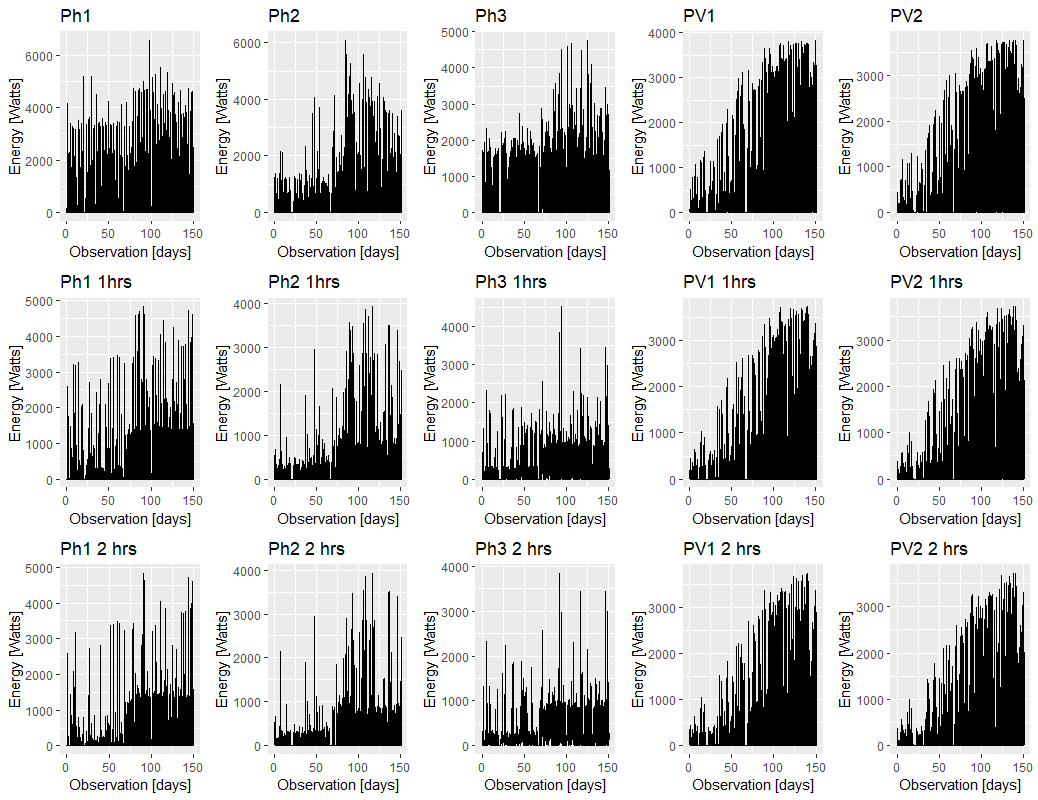
\includegraphics[width=0.9\textwidth]{dfulltimeseries.png}
    \caption{The 15 time series used for forecasting}
    \label{fulltimeseriesfigure}
\end{figure}

As can be seen, the first row of figure \ref{fulltimeseriesfigure} presents the original time series (just with the negative values cleaned).
The second row shows the down sampled time series, the sampling frequency here being one hour. Finally, the last row of the grid shows the time series down sampled with the frequency of two hours.

One can easily observe that the columns do not lose their shape by down sampling, which is a good thing, indicating that we didn't loose to much information from the data in the process. It should be noted how similar the \texttt{Ph1}, \texttt{Ph2} and \texttt{Ph3} time series are. \texttt{PV1} and \texttt{PV2} look much alike as well.

One can also observe from the plots that the data is still too dense. Even when using a sample frequency of two hours it is almost impossible to graphically analyze it and to draw any conclusions from it. So in order to apply the concepts discussed in the first chapter of this paper, for example to analyze the autocorrelation plot or the partial autocorrelation plot and decide on the parameters of the ARIMA model, I have to find an alternative way of analyzing the data.

This alternative way consists of breaking the data into representative chunks and then the analysis is done on those chunks and generalized to the whole time series. This process will be repeated 15 (fifteen) times, as many times as we have time series. As such, the data will be analyzed week by week and the patterns found for a week will be used to model the entire period of five months. Since electricity consumption or production patterns do not change very rapidly, such an approach is valid because we can generalize from a period of one week to the full period of five months. The consumption and production patterns will change ever so slightly that the algorithm will not notice any change. A household's schedule will only vary when there are unexpected events or changes in schedule and it is safe to assume that these do not happen too often, so the conclusion is that the schedule for a household keeps the same structure over a five month period as for a single (repeated) week.

If still there is any noticeable change, we could account for it by only taking into account one week and predicting the next several days, then by moving to the next week, modeling it using ARIMA and predicting the next days and repeating the process until we have processed the entire time series I would be able to cover the whole analyzed period without having to relay on the representativeness of a single week for the full data. In order to keep the above assumptions (although valid) to a minimum I have chosen this way of working with the data.

In summary, in order to be able to analyze the data I have looked at pieces of it, each piece being approximately the size of a week, and in order to avoid assumptions about the representativeness of that week, we always model with ARIMA a single week and produce forecasts for several days. This approach also falls in line with the Pareto principle, having approximately a week for training and several days for testing, presented also in listing \ref{actualKcode} via the \texttt{best.traindays} and \texttt{best.testdays}. The exact size for the training days and test days is determined as explained in section \ref{arimaincode}. As we will see in section \ref{methodologysection} this "week by week" forecasting approach is also useful in parallelizing the code. The code is embarrassingly parallel since every data chunk is independent of the previous or the next chunk. I can create an ARIMA model for a week and produce forecasts from it without influencing in any way the model and predictions for the previous or next week, for which all the data is independent. Of course the parallelization was done using the \texttt{foreach}\footnote{\url{https://cran.r-project.org/package=foreach}} \& \texttt{doParallel}\footnote{\url{https://cran.r-project.org/package=doParallel}} R packages.

\section{Methodology} \label{methodologysection}
This section deals takes all the presented pieces and puts them together. All the steps taken towards finding and fitting a proper ARIMA model will now be explained in logical order along with the decisions taken at every step in order to facilitate forecasting of electrical energy consumption and production.

First of all, during the modeling and forecasting process no distinction is made between the consumption of energy and the production of it. Both are treated as similar time series. This is possible because both are measured in the same units and are captured at the same intervals (the sampling frequency of the data set is five minutes). Thus the modeling and prediction process for the consumption and production doesn't have to be different, only the conclusions drawn will have to be different since the two processes are driven by different causes.

For reasons explained previously in section \ref{datasetsection} I will not use directly at the original time series in the data set, instead I will try to use the down sampled time series in order to be able to properly interpret the plots, since the high frequency time series yields plots that are way too dense to be interpreted. Also this is done because forecasting the original time series with ARIMA is very time consuming due to the high frequency of the data points and due to the sheer amount of data points available in a single time series (around 43200 points per time series). Hence I will use the down sampled time series, with sampling frequency of one and two hours respectively to be able to interpret the plots. I will use only chunks of one week to find the ARIMA parameters that properly fit the data and then forecast several days ahead, this process is then repeated, week by week, until all the data was fit and forecast. In summary: I will analyze a chunk of data (the down sampled data), approximately the size of a week, try to come up with proper ARIMA parameters for that respective week, then forecast the next several days (the size of the chunk and the size of the forecast horizon will be set to match the Pareto principle). The found parameters for ARIMA will be kept constant (considering that the model is representative for the whole data), but the model will then be re-fit for every next chunk of data from the time series, hence avoiding the assumption that the data doesn't change (or changes ever so slightly that it doesn't matter). This process will be repeated as many times as necessary, also yielding the embarrassingly parallel nature of the code, hence speeding things up a bit.

In what follows I will start walking through the steps necessary to model and forecast with ARIMA by actually giving an example for one of the time series. I will use as example the last week of the series \texttt{Ph3} sampled every two hours.

I start by analyzing a chunk of the data equivalent to the last week from the data since if we need to forecast what comes next, this week might prove to be the closest approximation there is. The simplest prediction one can make is to say that the future will look like the past, I will try to improve on this by finding an appropriate ARIMA model.

\begin{figure}[h]
    \centering
    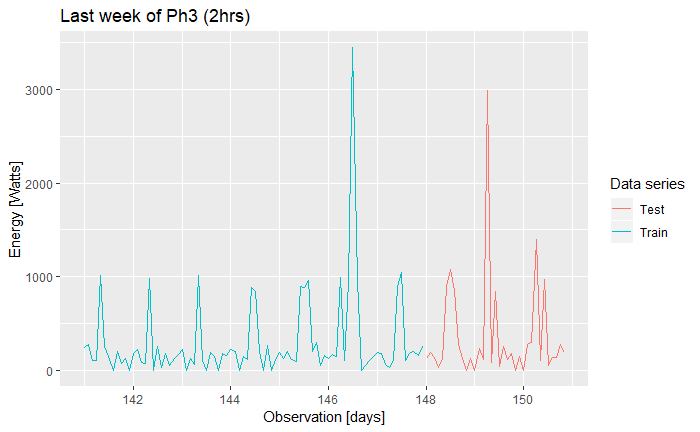
\includegraphics[width=0.75\textwidth]{dlastweek2hrsph3}
    \caption{Last week of the Ph3 data sampled every two hours}
    \label{dlastweek2hrsph3}
\end{figure}

For reference, the last week of the data can be seen in figure \ref{dlastweek2hrsph3}.
With blue I have represented the training data and the red line represents the test data for out-of-sample testing of the fitted model. The training data consists of 10 days and the test data of three days.

At a first glance from this figure we can observe that each day has a peak of consumption by which it can be easily recognized. We can see that the sixth day of the week is exceptionally large from the point of view of energy consumption. This data being gathered in Germany, we can be sure that this is a Saturday, hence a plausible explanation is that, indeed, this consumption is valid, and that the spike is not a glitch of the measurement or sampling system, since for a typical household everybody is at home on Saturdays and the consumption of electricity is expected to increase in such a case. This assumption is also confirmed by looking at other weeks from the data, all show the same spike on Saturdays, hence we cannot categorize it as an outlier due to measurement errors.

The nature o the data is further revealed by looking at the seasonal plot and subseries plot shown in figures \ref{dlastweek2hrsph3seasonal} and \ref{dlastweek2hrsph3subseries} respectively.

\begin{figure}[h]
    \centering
    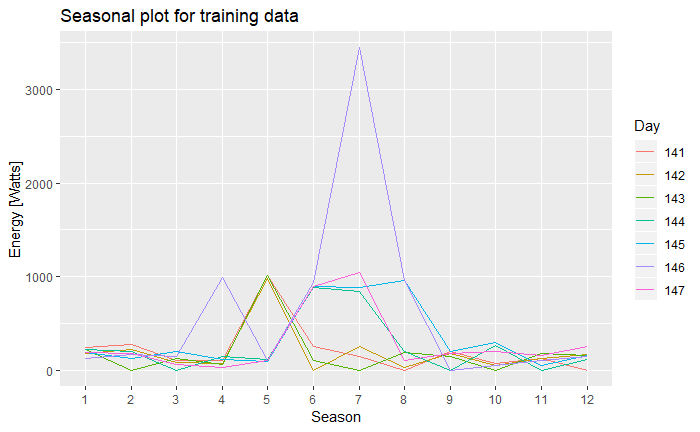
\includegraphics[width=0.75\textwidth]{dlastweek2hrsph3seasonal}
    \caption{Last week of the Ph3 data shown by seasons}
    \label{dlastweek2hrsph3seasonal}
\end{figure}

Both of these plots can be interpreted as explained in section \ref{seasonaldatasection}.
The seasonal plot, takes the time series data and arranges it in seasons, in this case two hour seasons. This can be seen on the X axis, which has 12 points. Because the training data contained seven days worth of data, in figure \ref{dlastweek2hrsph3seasonal} we see seven distinct time series each being a different day. Note that in order to convert the season to day hours we have to multiply by two, hence the seasonality of the data becomes obvious because each day there is an increase in electricity consumption after sunrise, starting with 06:00 in the morning and diminishing in the evening.

\begin{figure}[h]
    \centering
    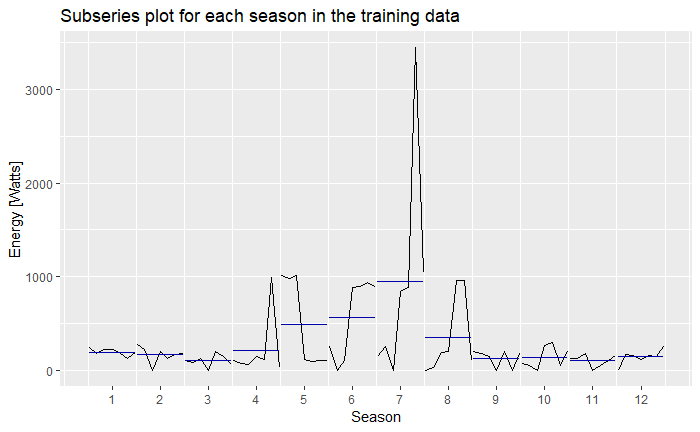
\includegraphics[width=0.75\textwidth]{dlastweek2hrsph3subseries}
    \caption{Last week of the Ph3 data shown by subseries}
    \label{dlastweek2hrsph3subseries}
\end{figure}

In the sub series plot the original data in split into seasons as well. Similarly the X axis also shows 12 points.
Each season on the plot is represented as an individual time series. Each observation belonging to the same season in a day is arranged in its respective slot. Since the training data had seven days worth of data, each mini time series consists of seven points, each from a different day, but the same season. The blue line shows the mean of each sub series. This plot shows that the energy consumption increases around lunch hours, hence reaching the conclusion this time series has daily seasonality.
So for now we might expect a seasonal ARIMA model to best fit the data, this conclusion will be also helpful when generating the dummies for use with the \texttt{SARIMAX} model.

Directly from the time plot of the data one can see that there are no trends or level shifts that might make the data non-stationary. Hence we can quickly conclude that there is no need for transformations (like the general BoxCox transformation) or for differencing, be it seasonal or non-seasonal.

Next, I shall inspect the autocorrelation and partial autocorrelation of the data in order to establish the \texttt{AR} and \texttt{MA} terms of ARIMA. These will also provide confirmation that the decision not to transform or differentiate the data was accurate. Both the ACF and PACF plots are shown in figure \ref{dlastweek2hrsph3acfpacf}.

\begin{figure}[h]
    \centering
    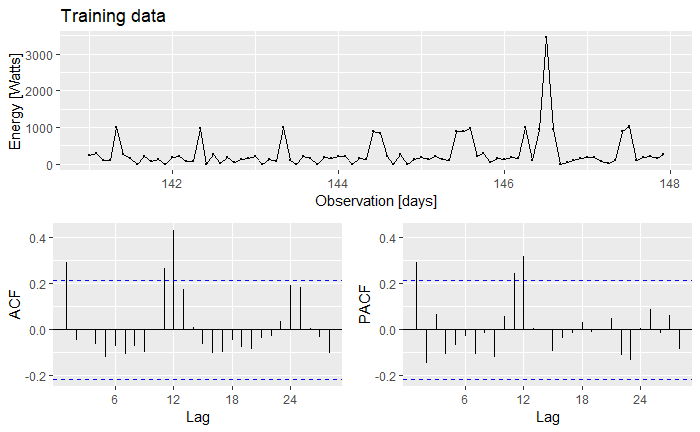
\includegraphics[width=0.75\textwidth]{dlastweek2hrsph3acfpacf}
    \caption{ACF and PACF of the data presented earlier}
    \label{dlastweek2hrsph3acfpacf}
\end{figure}

From the fact that the ACF plot doesn't slowly decay, but instead quickly drops, I get confirmation for the fact that the data is indeed stationary and it doesn't need differencing or seasonal differencing. So this settles the discussion for the $ d $ and $ D $ parameters of the seasonal ARIMA model. Both will be set to zero, $ d = 0 $ and $ D = 0 $.

From both the autocorrelation plot and the partial autocorrelation plot one can decide whether the model needs \texttt{AR} or \texttt{MA} terms.
According to what was presented in section \ref{choosingarandmasection} with regards to choosing the $ p $ or $ q $ parameters and to the ACF and PACF plots shown in figure \ref{dlastweek2hrsph3acfpacf} I decide that this data needs one \texttt{AR} term and one \texttt{SAR} term. So we will have $ p = 1 $ and $ P = 1 $. First of all, the ACF shown a sinusoidal form: positive for the first lag, negative around lag 6 and then positive again on lag 12, negative at lag 18 and back over zero around lag 24, a strong indication of an auto-regressive model. The order of the model can be deduced from the PACF plot, which has only one significant lag, then only non-significant ones, hence $ p = 1 $ is a good decision. The \texttt{SAR} order $ P = 1 $ is chosen this way since we have significant spikes at seasonal lags 12 and almost significant spikes at lag 24. Please keep in mind that there are only 12 observation per day, since the data presented here is sampled with a frequency of two hours, so these significant spikes match a full day, a 24 hour period, thus matching our initial observations from the seasonal and seasonal subseries plots in figures \ref{dlastweek2hrsph3seasonal} and \ref{dlastweek2hrsph3subseries} respectively.

With this I have arrived at an initial model that looks like this: $ ARIMA(1, 0, 0)(1, 0, 0)[12] $. That is, a first order non-seasonal and seasonal auto-regressive ARIMA model with no differences and no moving average. The seasonal period is 12, every 12th observation a new day starts within the data.

The model fitting code is shown in listing \ref{modelfittingcode}.

\begin{listing}[h]
    \begin{minted}{R}
fit <- Arima(data, order=c(1, 0, 0), seasonal=c(1, 0, 0))
    \end{minted}
    
    \caption{Model fitting code}
    \label{modelfittingcode}
\end{listing}

Now I shall see how this model behaves and if it captures all the information in the data. This is done first by inspecting the residuals, see figure \ref{dlastweek2hrsph3residuals}.

\begin{figure}[h]
    \centering
    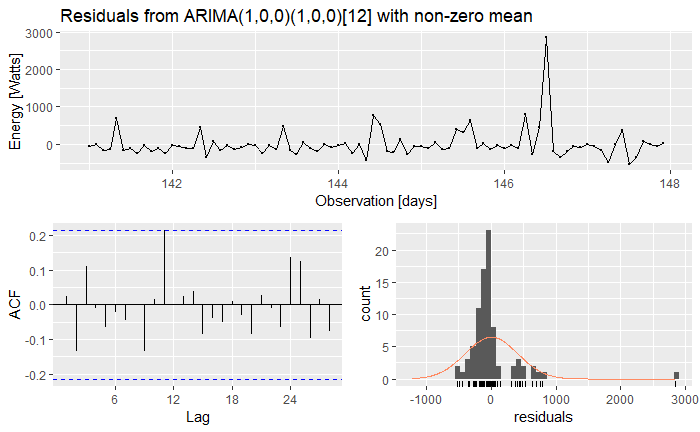
\includegraphics[width=0.75\textwidth]{dlastweek2hrsph3residuals}
    \caption{Residuals obtained after fitting the model}
    \label{dlastweek2hrsph3residuals}
\end{figure}

From the time plot of the residuals (the first row of the figure) one can clearly see that there are some peaks in the data that we didn't get information out of. This also can be seen in the ACF plot (lower left in the figure \ref{dlastweek2hrsph3residuals}) since at lag 11 there is an almost significant peak. Still, the peak is not high enough to be significant and one significant peak might just be ignored since we see more than 20 lags in the plot, hence we would still be in the limits of the 95\% confidence interval. With the exception of the extremely high peak on the sixth day, the histogram of the residuals looks good as well. 

\begin{figure}[h]
    \centering
    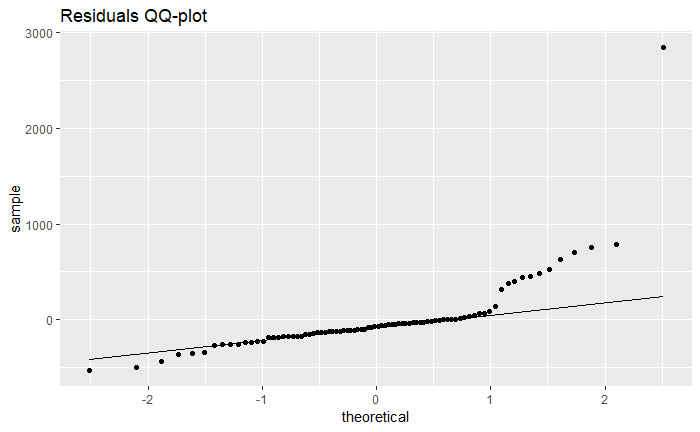
\includegraphics[width=0.75\textwidth]{dlastweek2hrsph3qq}
    \caption{QQ plot of the residuals}
    \label{dlastweek2hrsph3qq}
\end{figure}

Now if we look at the QQ plot of the residuals (shown in figure \ref{dlastweek2hrsph3qq}) we see that indeed they look normal.

So I might say that the model nicely fits the data and that the residuals show us that pretty much of the information in the data has been extracted, but there could still be room for improvement, more information can be extracted from the data.

In order to properly compare with future models, I have used the Ljung-Box test statistic, for which I obtained a value of $ Q^* = 10.787 $. As specified in the theoretical section \ref{ljungboxsection} the $ Q^* $ value is lower for those models with less residual correlation. After fitting other versions of the model we will be able to compare them by using this measure as well as the forecast accuracy.

Finally, in listing \ref{forecastingcode} one can see the code used to forecast using the model we have found so far.

\begin{listing}[h]
    \begin{minted}{R}
fcast <- forecast(fit, h=36)
    \end{minted}
    
    \caption{Forecasting code}
    \label{forecastingcode}
\end{listing}

The \texttt{h} parameter is chosen to match the number of observations that fit in the three days we need to predict. With a frequency of sampling of two hours and three test days, that leads to $ h = 3 \cdot 12$

The accuracy of the $ ARIMA(1, 0, 0)(1, 0, 0)[12] $ model on the last week of the \texttt{Ph3} (two hour sampling frequency) time series is presented in table \ref{accuracyofinitialmodel}.

\begin{table}[h]
    \begin{tabular}{|c|c|c|c|}
        \hline
        & \textbf{ME} & \textbf{RMSE} & \textbf{MAE} \\
        \hline
        \textbf{Training set} & 4.050695 & 403.3290 & 215.3303\\
        \hline
        \textbf{Test set} & 77.981474 & 560.1617 & 295.7273 \\
        \hline
    \end{tabular}
    \centering
    \caption{Accuracy of the $ SARIMA(1, 0, 0)(1, 0, 0)[12] $ model}
    \label{accuracyofinitialmodel}
\end{table}

From this table we are mainly interested in the accuracy on the test set. That is, the three days following the week we trained our model on. The three measures correspond to what was presented in section \ref{accuracymeasuressection}. Namely the mean error, mean absolute error and the root mean squared error.

Lastly, in figure \ref{dlastweek2hrsph3forecasts} I have shown the actual forecasts produced by the model.

\begin{figure}[h]
    \centering
    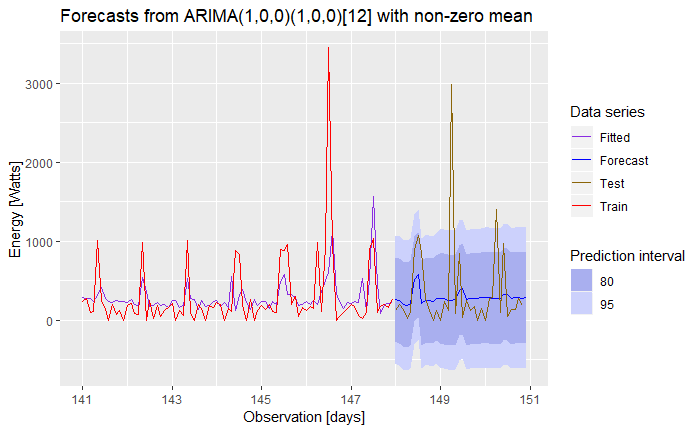
\includegraphics[width=0.75\textwidth]{dlastweek2hrsph3forecasts}
    \caption{Forecasts from the $ SARIMA(1, 0, 0)(1, 0, 0)[12] $ model}
    \label{dlastweek2hrsph3forecasts}
\end{figure}

With red we can see the original training data, while brown was used to represent the original test data from the \texttt{Ph3} time series.
The violet line was used to show the fitted values of the model and the blue line, shown for the last three days of the plot, shows the forecast values. The darker shade of blue shows the 80\% confidence interval for the predictions and the lighter shade of blue shows the 95\% confidence interval for the predictions. Regardless of the position of the line in the shaded areas, for the 80\% confidence interval we are are 80\% sure that any prediction would fall in that range, while for the 95\% prediction interval we are 95\%sure that the prediction will fall in that specific range. One can easily see that the confidence interval where the confidence is higher is larger as well, since the possibilities are more numerous.

Please note that the negative prediction intervals are due to the way these are computed: the point forecast plus/minus the standard deviation multiplied by the 95\% or 80\% critical value of the two tailed Z distribution, this usually means the point forecast plus/minus twice the standard error. For more details see section \ref{cirticalvaluesection}. The lower part of the interval should be limited at zero during the
interpretation of the results, but this is not done on the plot due to symmetry and graphical reasons.

The forecasts plot shows us that the fitting phase was successful, the data is closely modeled, but not identical, this is the ideal scenario since we do not want to fall into the trap of over fitting the data without being able to generalize from it. The forecasts on the other hand only look good for the duration of the first day, then regressing to the mean of the data without actually taking the form of the valleys and peaks of the test data. This is one reason for which I have varied the number of training and test days, in order to be able to extract the best results out of a similar model. The full results will be shown in section \ref{resultssection}.

Since during the model fitting phase I reached the conclusion that the model might be slightly improved, I'm going to demonstrate both the dynamic harmonic regression and forecasting with dummies in order to see if I can extract more information from the seasonal peaks in the residuals that yield an almost-significant spike at lag 11. We're going to compare the Ljung-Box test results for each of the models and, more importantly the accuracy and final forecasts of the models.

According to sections \ref{dynamicharmonicregression}, \ref{arimaincode} and to listing \ref{actualKcode} I have varied the number of Fourier terms to be included in this model and the best result was achieved for $ K = 2 $. The fitted model is shown in listing \ref{modelfittingcodeFourier}. As can be seen from the code, the seasonal part of the code has been replaced by the Fourier terms, which should handle seasonality by themselves.

\begin{listing}[h]
    \begin{minted}{R}
    fit <- Arima(data, order=c(1, 0, 0), xreg=fourier(data, K=2))
    \end{minted}
    
    \caption{Model fitting code for the second variation, including Fourier terms instead of a seasonal model}
    \label{modelfittingcodeFourier}
\end{listing}

The $ Q^* $ for obtained for this model is $ 13.731 $, which is higher than what was obtained for the initial model ($ Q^* = 10.787 $).

\begin{figure}[h]
    \centering
    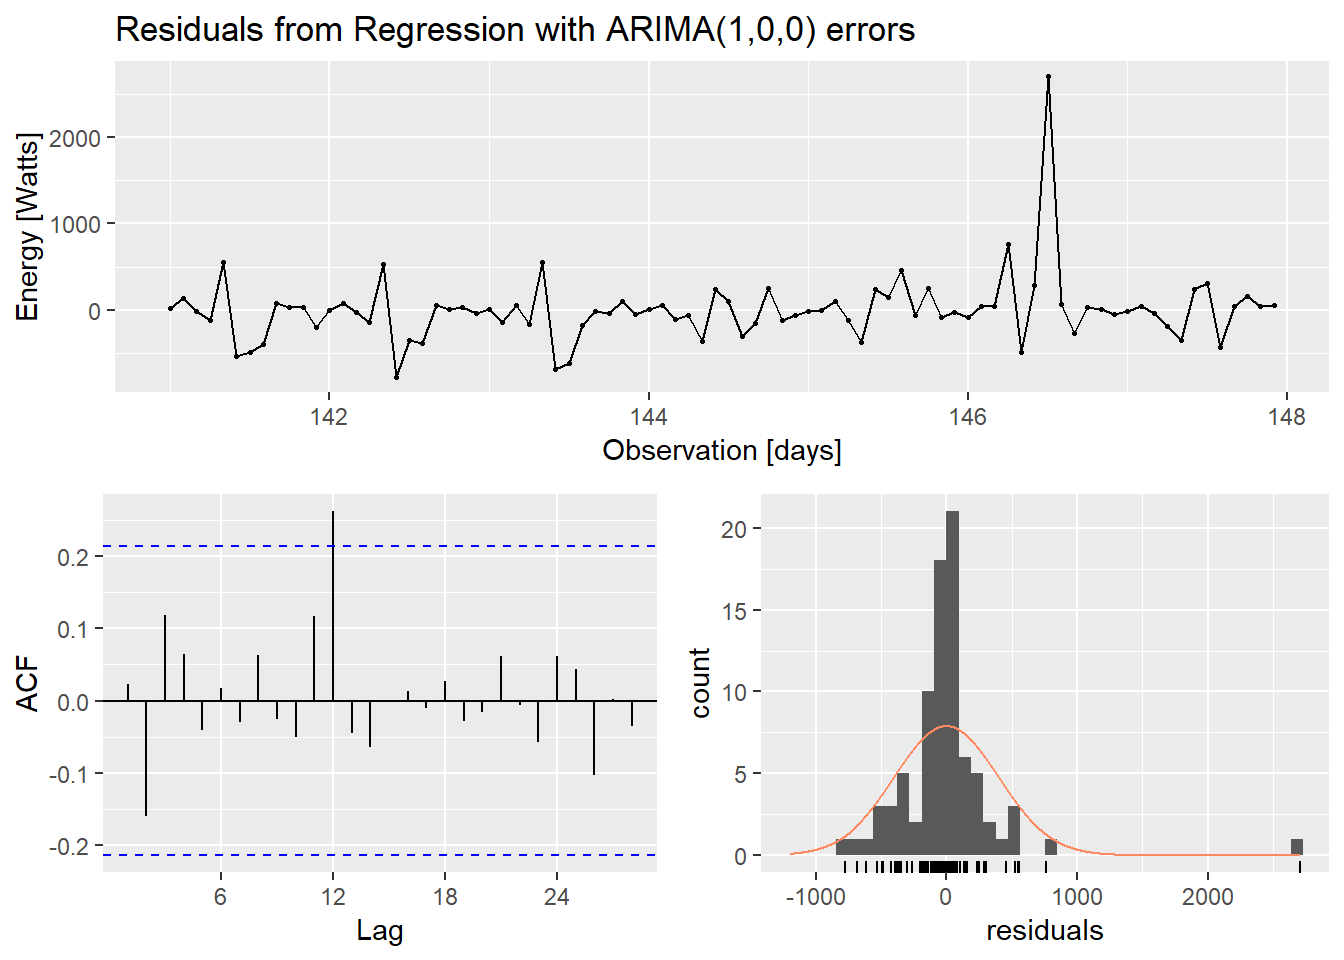
\includegraphics[width=0.75\textwidth]{dlastweek2hrsph3residualsFourier}
    \caption{Residuals of the $ ARIMAX(1, 0, 0) $ model with Fourier terms}
    \label{dlastweek2hrsph3residualsFourier}
\end{figure}

Looking at the residuals in figure \ref{dlastweek2hrsph3residualsFourier} we can see that the ACF presents a significant spike at lag 12 and there are still noticeable patterns in the data. This is clearly not an improvement over the initial model, but for completeness table \ref{accuracyofFouriermodel} and figure \ref{dlastweek2hrsph3forecastsFourier} show the accuracy of this model and its forecasts.

\begin{table}[h]
    \begin{tabular}{|c|c|c|c|}
        \hline
        & \textbf{ME} & \textbf{RMSE} & \textbf{MAE}\\
        \hline
        \textbf{Training set} & -0.0493095 & 397.5424 & 215.1969 \\
        \hline
        \textbf{Test set} & 63.5939328 & 601.4848 & 311.4614 \\
        \hline
    \end{tabular}
\centering
\caption{Accuracy of the $ ARIMAX(1, 0, 0) $ model with Fourier terms}
\label{accuracyofFouriermodel}
\end{table}

\begin{figure}[h]
    \centering
    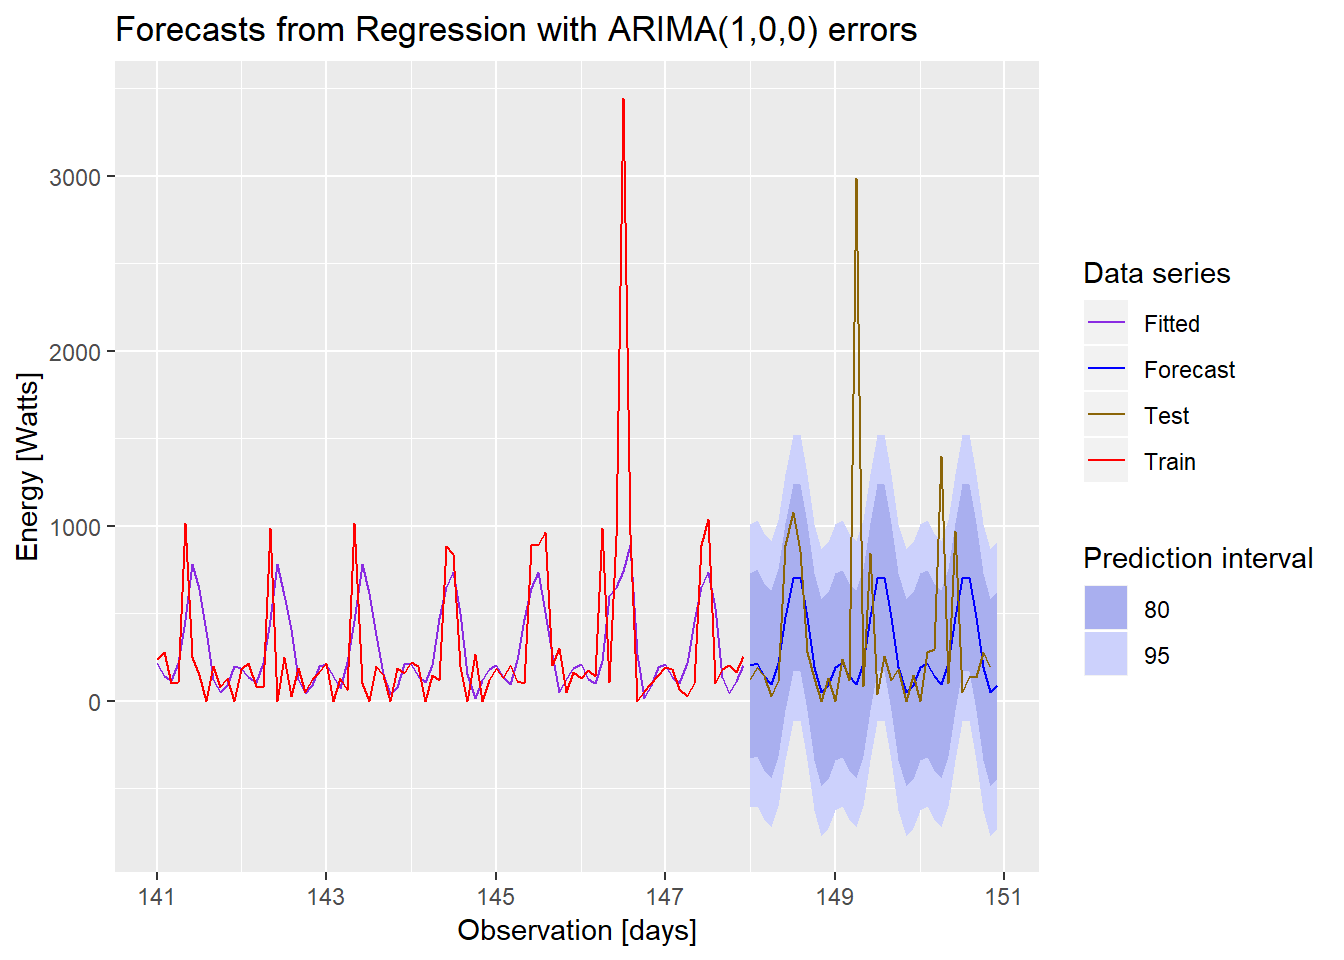
\includegraphics[width=0.75\textwidth]{dlastweek2hrsph3forecastsFourier}
    \caption{Forecasts from the $ ARIMAX(1, 0, 0) $ model with Fourier terms}
    \label{dlastweek2hrsph3forecastsFourier}
\end{figure}

Only the mean error of the model is slightly improved, all other measures of accuracy are worse in this modified model. Still this model does show a better shape for the predicted period, being able to show the seasonality in the produced forecasts, as well as in the fitted data.

The next model I have investigated is a dummies based model, derived from the initial one, the code for fitting it can be seen in listing \ref{modelfittingcodeDummies}.

\begin{listing}[h]
    \begin{minted}{R}
    fit <- Arima(data, order=c(1, 0, 0), seasonal=c(1, 0, 0),
        xreg=getNthObsDummies(5, 4, length(data), frequency(data)))
    \end{minted}
    
    \caption{Model fitting code for the third variation, using dummies}
    \label{modelfittingcodeDummies}
\end{listing}

From the listing, the parameters for \texttt{getNthObsDummies} are \texttt{nth = 5}, \texttt{dummyLen = 4}, \texttt{len} is the same length as the data, \texttt{numObsPerDay = 12}. This means that we want to separately see the influence of the 5th observation up to the 9th one, in hours this means from 10:00 to 18:00, this decision was based on the seasonal plots shown in figures \ref{dlastweek2hrsph3seasonal} and \ref{dlastweek2hrsph3subseries}. There we can see the variations starting to appear around the 5th observation and diminishing around the 9th observation.

The residuals for this model can be seen in figure \ref{dlastweek2hrsph3residualsDummies}.

\begin{figure}[h]
    \centering
    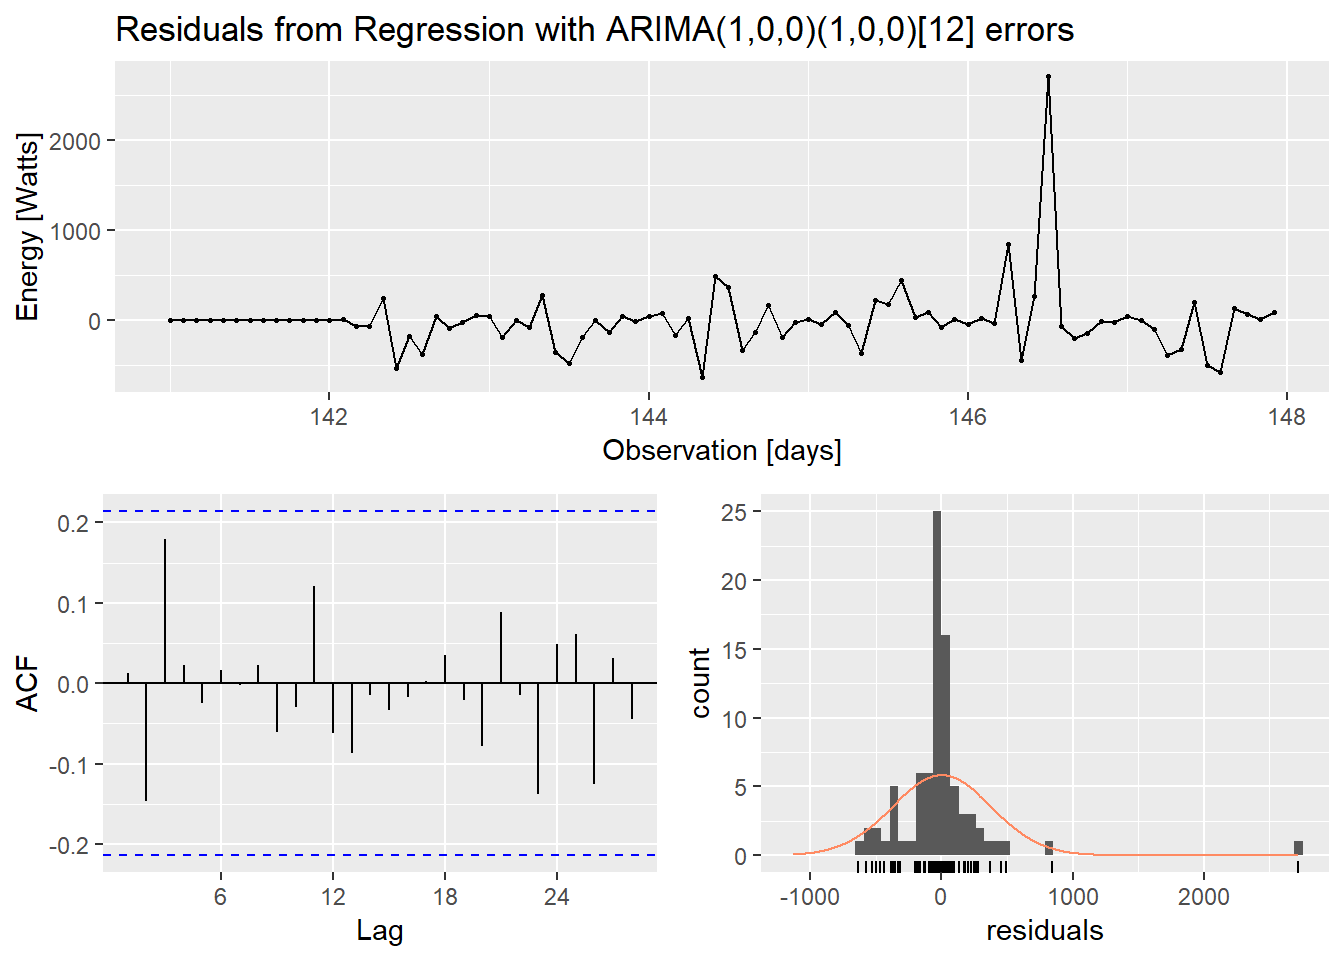
\includegraphics[width=0.75\textwidth]{dlastweek2hrsph3residualsDummies}
    \caption{Residuals of the $ SARIMAX(1, 0, 0)(1, 0, 0)[12] $ model with mid-day dummies}
    \label{dlastweek2hrsph3residualsDummies}
\end{figure}

Here we no longer see an almost-significant spike around lag 12 in the autocorrelation plot, backed up by the fact that there are no noticeable patterns in the time plot of the residuals I can say that this model already performs better, only through the point of view of the "learned information" from the data. This is also in accordance with a lower $ Q^* $ value from the Ljung-Box test for residual independence. The obtained value for this model is $8.1016 $ (the obtained value for the initial model was $ Q^* = 10.787 $).

\begin{table}[h]
    \begin{tabular}{|c|c|c|c|}
        \hline
        & \textbf{ME} & \textbf{RMSE} & \textbf{MAE}\\
        \hline
        \textbf{Training set} & 0.0036377 &	375.3853 &	178.3065 \\
        \hline
        \textbf{Test set} & 50.3116754 &	583.6319 &	300.6943 \\
        \hline
    \end{tabular}
    \centering
    \caption{Accuracy of the $ SARIMAX(1, 0, 0)(1, 0, 0)[12] $ model with mid-day dummies}
    \label{accuracyofDummiesmodel}
\end{table}

The accuracy of the model, shown in table \ref{accuracyofDummiesmodel} also displays smaller errors than for the initial model (see table \ref{accuracyofinitialmodel}), with the exception of the mean absolute error, but the difference is only 5 units, which can be safely ignored.

Regarding the forecasts, they are also satisfactory, the seasonal nature of the data was projected into the future and the fit of the model for the training data is good as well, taking the shape of the red line, as observed in figure \ref{dlastweek2hrsph3forecastsDummies}.

\begin{figure}[h]
    \centering
    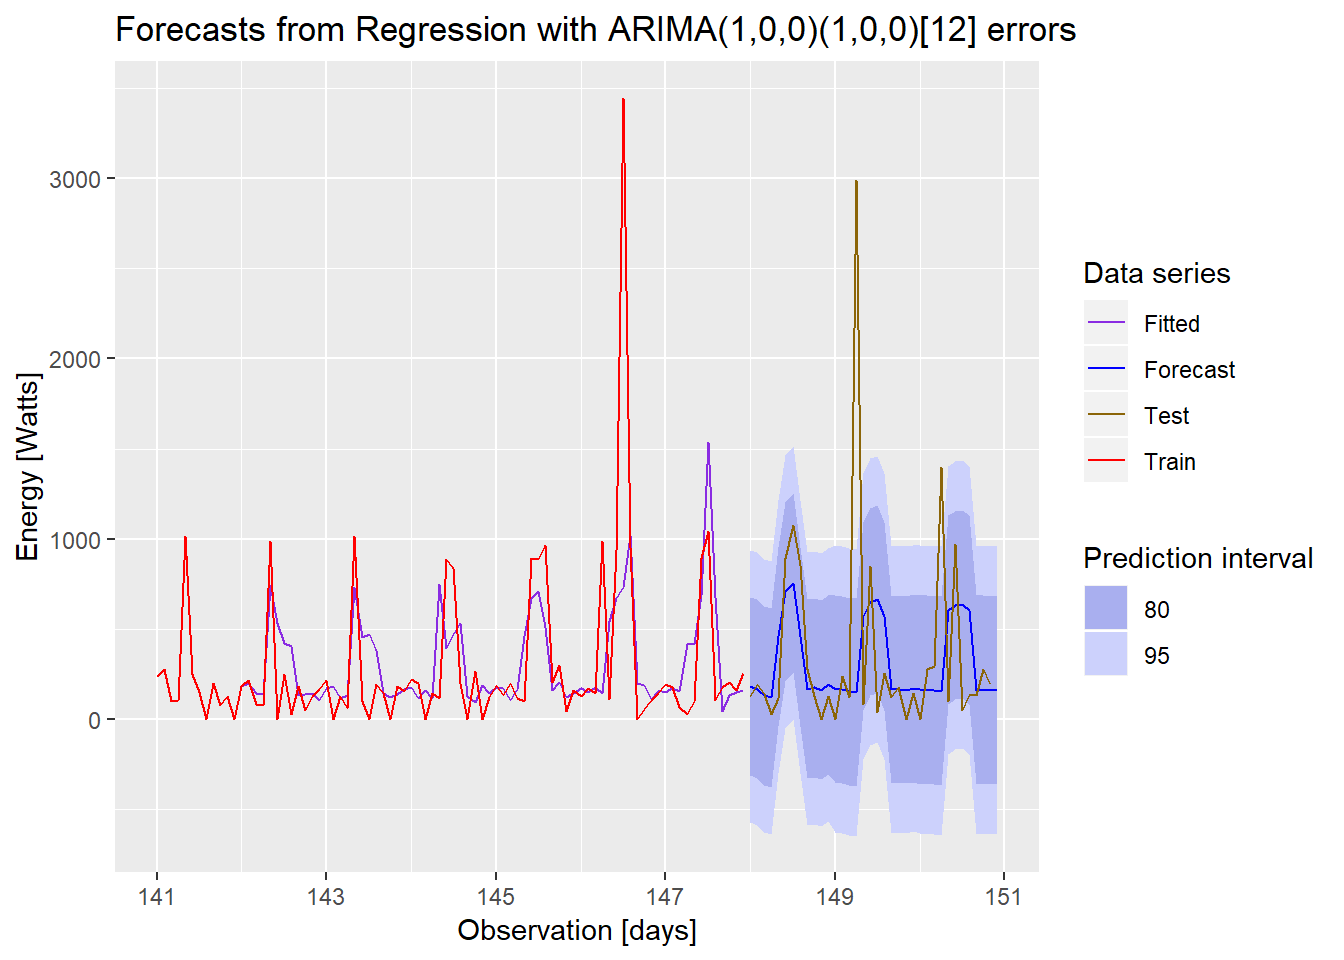
\includegraphics[width=0.75\textwidth]{dlastweek2hrsph3forecastsDummies}
    \caption{Forecasts from the $ SARIMAX(1, 0, 0)(1, 0, 0)[12] $ model with mid-day dummies}
    \label{dlastweek2hrsph3forecastsDummies}
\end{figure}

Having found a good performing model on a single chunk of data it is time to try and apply this model to the entire time series.
For the \texttt{Ph3} time series with the sampling frequency of two hours I have, unfortunately, found that this model is not the best, but instead a combination of ARIMA with dummies and Fourier terms is. The way to reach such a complex combination is by starting from an empirical observation, such as we already have here and then algorithmically explore several ones.

Apart from combining dummies with dynamic harmonic regression, we also have to vary the parameters of the individual parts of the model.
One such part was presented in sections \ref{dynamicharmonicregression} and \ref{arimaincode} and in listing \ref{actualKcode}, namely the choosing of the number of Fourier terms to include in the model. Another part is to try to find the best range for the dummies. Using the above example, starting at the 5th observation up to the 9th might not be the optimal choice, instead we should try a different starting point and ending point in the hope that the accuracy of the model will be better (that is the errors will be generally lower). The third important point of configuration is the number of training and test days, which again is algorithmically computed by varying the number of test and train days to achieve the smallest errors. 

An example piece of code that varies the configuration of the dummies can be seen in listing \ref{codedummiesconfiguration}.

\begin{listing}[h]
    \begin{minted}{R}
best.fcast.dummy.2hrsPh3 <- NULL
best.startDummy <- 0
best.lenDummy <- 0
    
for(startDummy in 4:8)
{
    for(lenDummy in 1:5)
    {
        obsDummies.<- getNthObsDummies(startDummy, lenDummy, h, frequency(data))
        
        # fit & forecast, keep the best model and dummies configuration
    }
}
\end{minted}

\caption{Code snippet for the best dummies configuration}
\label{codedummiesconfiguration}
\end{listing}

The lower and upper limits for the \texttt{startDummy} and \texttt{lenDummy} variables were chosen to match the time the values started to increase (and respectively to decrease) in the seasonal and seasonal sub-series plots (see \ref{dlastweek2hrsph3seasonal} and \ref{dlastweek2hrsph3subseries}) with allowance for some variability.

With this information in mind, one the best performing model (for the entire \texttt{Ph3} data, with two hour sampling frequency) I have found is: $ ARIMA(1, 0, 0) $ with 10:00 to 12:00 dummies (one dummy at the 5th observation) and two Fourier terms ($ K = 2 $). The number of training days was kept at 7 and the forecast days at 3. The full time series are forecast by fitting the found model on chunks of (in this particular case) 7 days and predicting the energy consumption or production (consumption in this case) for the next three days. The accuracy for the full time-series is computed by averaging the accuracy for each chunk of forecasts. Please keep in mind that these figures are particular to the \texttt{Ph3} time series, with two hour sampling frequency, a summary of the best performing models and their parameters on all sampling frequencies and time series will be given in section \ref{resultssection}.

The accuracy for the model presented earlier is shown in table \ref{accuracyoffull2hrsph3} and the forecasts for the entire span of time is shown in figure \ref{d2hrsph3fourierDummiesforecast}.

\begin{table}[h]
    \begin{tabular}{|c|c|c|c|}
        \hline
        & \textbf{ME} & \textbf{RMSE} & \textbf{MAE}\\
        \hline
        \texttt{2hrs Ph3} & 7.063614 &	318.2331 &	179.0269 \\
        \hline
    \end{tabular}
    \centering
    \caption{Accuracy of the $ ARIMAX(1, 0, 0) $ model with two Fourier terms and one dummy}
    \label{accuracyoffull2hrsph3}
\end{table}
    
    
\begin{figure}[h]
    \centering
    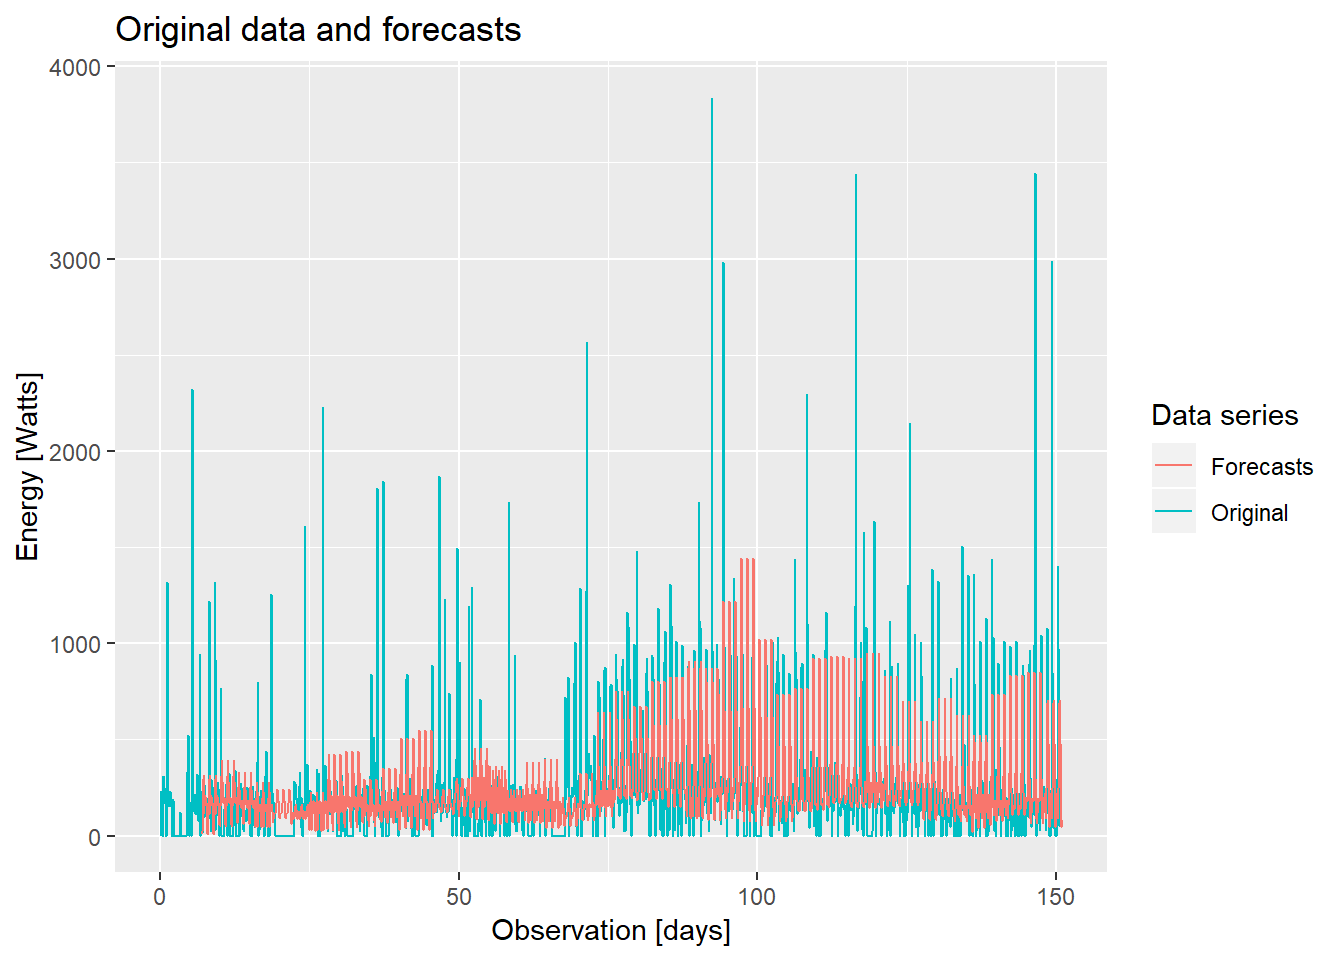
\includegraphics[width=0.9\textwidth]{d2hrsph3fourierDummiesforecast}
    \caption{Forecasts from the $ ARIMA(1, 0, 0) $ model with two Fourier terms and one dummy}
    \label{d2hrsph3fourierDummiesforecast}
\end{figure}

As can be seen in figure \ref{d2hrsph3fourierDummiesforecast}, no forecasts are made for the first chunk of the data (the first training days) since there is no prior data to that. One could substitute the forecasts for that period with the fitted values, but for accuracy I chose not to do such a thing.

The above explanation can now be applied for any of the 15 time series: the five original ones, \texttt{Ph1}, \texttt{Ph2}, \texttt{Ph3}, \texttt{PV1}, \texttt{PV2} and their sub-sampled versions, with sampling frequencies of one and two hours (the original sampling frequency was 5 minutes). The results I have reached in doing so are presented in section \ref{resultssection}.

\section{Difficulties in implementation of the methodology}
No difficulty in the theoretical part since it is well established and widely used by now.
But the technical part, parallelization, errors, etc

data too frequent, arima takes very long to run -> parallelization and down sampling
Say about "down sampling" of data and why is it necessary.
the methodology explains why I can parallelize the code

Data too long, forecast by chunks, which are independent. and show I I brought them together, also th three days worth of predictions decay very fast, hence we try several possibilities.

down-sampling the data since it was too frequent + R code

\section{Results} \label{resultssection}
%TODO -Which are the main results of your paper and application areas ?

%TODO: tables with results and attached plots
Show only the best results on the down sampled time series and all of them on the original data. complete with running times as well.
How many train days and test days are best to forecast?

Summary of time-series (more 15 of them, as line sin table) and models chosen, time to run, train/test days, fourier, dummies, and how many models are best for a given time series.


compare with other methods (NN and markov)


\section{Future work}
%TODO -Which are the main steps to develop your research in the future ?
%TODO: avergage, naive, snaive on embedded
%TODO: errors cause

\section{Conclusions}
%TODO: abstract, introduction, R, data, methodology, ARIMA, results, future work

arima is not really suited for high frequency data
consumption vs production of electrical energy
\newpage
\bibliographystyle{plain}
\bibliography{bibliografie}

\end{document}
